 %% abtex2-modelo-trabalho-academico.tex, v-1.9.2 laurocesar

%% Copyright 2012-2014 by abnTeX2 group at http://abntex2.googlecode.com/ 
%%
%% This work may be distributed and/or modified under the
%% conditions of the LaTeX Project Public License, either version 1.3
%% of this license or (at your option) any later version.
%% The latest version of this license is in
%%   http://www.latex-project.org/lppl.txt
%% and version 1.3 or later is part of all distributions of LaTeX
%% version 2005/12/01 or later.
%%
%% This work has the LPPL maintenance status `maintained'.
%% 
%% The Current Maintainer of this work is the abnTeX2 team, led
%% by Lauro César Araujo. Further information are available on 
%% http://abntex2.googlecode.com/
%%
%% This work consists of the files abntex2-modelo-trabalho-academico.tex,
%% abntex2-modelo-include-comandos and abntex2-modelo-references.bib
%%
%------------------------------------------------------------------------
% ------------------------------------------------------------------------ 
% abnTeX2: Modelo de Trabalho Academico (tese de doutorado, dissertacao de
% mestrado e trabalhos monograficos em geral) em conformidade com 
% ABNT NBR 14724:2011: Informacao e documentacao - Trabalhos academicos -
% Apresentacao
% ------------------------------------------------------------------------
% ------------------------------------------------------------------------

\documentclass[
	% -- opções da classe memoir --
	12pt,				% tamanho da fonte
	openright,			% capítulos começam em pág ímpar (insere página vazia caso preciso)
	twoside,			% para impressão em verso e anverso. Oposto a oneside
	a4paper,			% tamanho do papel. 
	% -- opções da classe abntex2 --
	%chapter=TITLE,		        % títulos de capítulos convertidos em letras maiúsculas
	%section=TITLE,		        % títulos de seções convertidos em letras maiúsculas
	%subsection=TITLE,	        % títulos de subseções convertidos em letras maiúsculas
	%subsubsection=TITLE,           % títulos de subsubseções convertidos em letras maiúsculas
	% -- opções do pacote babel --
	english,			% idioma adicional para hifenização
	french,				% idioma adicional para hifenização
	spanish,			% idioma adicional para hifenização
        italian,                        % idioma adicional para hifenização
	brazil				% o último idioma é o principal do documento
	]{abntex2}

% ---
% Pacotes
% ---
% ---
% Pacotes básicos 
% ---
\usepackage[utf8]{inputenc}		% Codificacao do documento (conversão automática dos acentos)
\usepackage{lmodern}			% Usa a fonte Latin Modern			
\usepackage[T1]{fontenc}		% Selecao de codigos de fonte.
\usepackage{lastpage}			% Usado pela Ficha catalográfica
\usepackage{indentfirst}		% Indenta o primeiro parágrafo de cada seção.
\usepackage{color}				% Controle das cores
\usepackage{graphicx}			% Inclusão de gráficos
\usepackage{wallpaper}			% inclusao de imagens deslocadas
\usepackage{microtype} 			% para melhorias de justificação
\usepackage{url}
\usepackage[table,xcdraw]{xcolor}
\usepackage{tabularx}
\usepackage{minted}
\usepackage{amsmath,amssymb}
\usepackage{framed}
\usepackage[amsmath,framed]{ntheorem}
\usepackage{pdfpages}

% ---
		
% ---
% Pacotes adicionais, usados apenas no âmbito do Modelo Canônico do abnteX2
% ---
\usepackage{lipsum}				% para geração de dummy text
% ---

%---
% Pacote para listas em uma linha
%---
\usepackage{paralist}

% ---
% Epigrade
% ---
\usepackage{epigraph}

% Front end para amsthm (\declaretheorem)
\usepackage{thmtools}    

% ---
% Pacotes de citações
% ---
\usepackage[brazilian,hyperpageref]{backref}	 % Paginas com as citações na bibl
\usepackage[alf]{abntex2cite}	% Citações padrão ABNT

%TODO
\usepackage[colorinlistoftodos]{todonotes}
%\usepackage{ntheorem}

\usepackage{tablefootnote}


%%%%%%%%%%% syntax highlight %%%%%%%%%%%%%%%%%%%%%%%%%%%%%%%%%%%%%%%%%%%%%%%%%%%%%
\usepackage{listings}
\definecolor{maroon}{rgb}{0.5,0,0}
\definecolor{darkgreen}{rgb}{0,0.5,0}
\definecolor{deepblue}{rgb}{0,0,0.5}
\definecolor{deepred}{rgb}{0.6,0,0}
\definecolor{purple}{rgb}{0.5,0,0.5}
\definecolor{deepgreen}{rgb}{0,0.5,0}
%%%%%%%%%%%%%%%%%%%%%%%%%%%%%%%%%%%%%%%%%%%%%%%%%%%%%%% 

\usepackage{tikz}
\tikzset{
  treenode/.style = {shape=rectangle, rounded corners,
                     draw, align=center,
                     top color=white, bottom color=blue!20},
  root/.style     = {treenode, font=\Large, bottom color=red!30},
  env/.style      = {treenode, font=\ttfamily\normalsize},
  dummy/.style    = {circle,draw}
}


% ---
% MACROS
% ---
% --- 
% CONFIGURAÇÕES DE PACOTES
% --- 

% ---
% Configurações do pacote backref
% Usado sem a opção hyperpageref de backref
\renewcommand{\backrefpagesname}{Citado na(s) página(s):~}
% Texto padrão antes do número das páginas
\renewcommand{\backref}{}
% Define os textos da citação
\renewcommand*{\backrefalt}[4]{
	\ifcase #1 %
		Nenhuma citação no texto.%
	\or
		Citado na página #2.%
	\else
		Citado #1 vezes nas páginas #2.%
	\fi}%
% ---

\newcommand{\traducao}[2]{``#1''\footnote{Tradução nossa de ``\emph{#2}''}}
\newcommand{\tabletraducao}[2]{``#1'' \tablefootnote{Tradução nossa de \emph{#2}.}}
\newcommand{\traducaoparcial}[2]{``#1'' \footnote{Tradução parcial nossa de \emph{#2}.}}
\newcommand{\csf}[2]{$\mathcal{#1}_\emph{#2}$}
\newcommand{\traduzcitacao}[4]{\begin{citacao}
#1\cite[#3]{#4}\footnote{Tradução de \emph{#2}}.
\end{citacao}
}

\newcommand{\disponivelem}[1]{\footnote{Disponível em \url{#1}}}
\newcommand{\sorensen}[2]{#1\disponivelem{#2}}
\newcommand{\ver}[1]{(ver \autoref{#1}, p.~\pageref{#1})}
\newcommand{\traducaoapud}[5]{``#1'' \apud[#3]{#4}{#5}\traducao{#2}}
\newcommand{\pressingtwo}[2]{$\mathcal{#1}'_{#2}$}
\newcommand{\pressingthree}[3]{$\mathcal{#1}'^{#3}_{#2}$} 
\newcommand{\metafora}[2]{\scriptsize \MakeTextUppercase{#1} \normalsize, isto é, #2}
\newcommand{\verex}[1]{(ver Exemplo \autoref{#1}, p.~\pageref{#1})}
\newcommand{\idemibdem}{\emph{idem}, \emph{ibdem}}
\newcommand{\tempo}[2]{#1$'$#2$''$}

%%%%%%%%%%%%%%%%%%%%%%%%%%%%%%%%%%%%%%%%%%%%%%%%
% An example environment
%%%%%%%%%%%%%%%%%%%%%%%%%%%%%%%%%%%%%%%%%%%%%%%%
\theoremheaderfont{\normalfont\bfseries}
\theorembodyfont{\normalfont}
\theoremstyle{break}
\def\theoremframecommand{{\color{deepred}\vrule width 5pt \hspace{5pt}}}
\newshadedtheorem{exa}{Exemplo}[chapter]
\newenvironment{example}[1]{%
		\begin{exa}[#1]
}{%
		\end{exa}
}


% ---
% Informações de dados para CAPA e FOLHA DE ROSTO
% ---
\titulo{Improvisações de códigos para análise de um algoritmo tonal no \emph{A Study in Keith} (2009) de Andrew Sorensen}
\autor{Guilherme Martins Lunhani}

\instituicao{Universidade Federal de Juiz De Fora -- UFJF
  \par
  Instituto de Artes e Design -- IAD
  \par
  Programa de Pós-Graduação em Artes Visuais, Música e Tecnologia}

\orientador[Orientador: ]{Prof. Dr. Luiz Eduardo Castelões}

\data{\today}

% \changes{Versão inicial }{2013/07/22 }{v0.0.3}
\tipotrabalho{Tese (Mestrado)}

% O preambulo deve conter o tipo do trabalho, o objetivo, 
% o nome da instituição e a área de concentração 
\preambulo{Dissertação corrigida para a banca de qualificação no Programa Mestrado em Artes, Cultura e Linguagens do Instituto de Artes e Design da Universidade Federal de Juiz de Fora (UFJF), linha de Artes Visuais, Musica e Tecnologia.}
%\EnableCrossrefs
%\CodelineIndex
%\RecordChanges

% ---
% Configurações de aparência do PDF final

% alterando o aspecto da cor azul
\definecolor{blue}{RGB}{41,5,195}

% informações do PDF
\makeatletter
\hypersetup{
     	%pagebackref=true,
		pdftitle={\@title}, 
		pdfauthor={\@author},
    	pdfsubject={\imprimirpreambulo},
	    pdfcreator={LaTeX with abnTeX2},
		pdfkeywords={abnt}{latex}{abntex}{abntex2}{trabalho acadêmico}, 
		colorlinks=true,       		% false: boxed links; true: colored links
    	linkcolor=blue,          	% color of internal links
    	citecolor=blue,        		% color of links to bibliography
    	filecolor=magenta,      		% color of file links
		urlcolor=blue,
		bookmarksdepth=4
}
\makeatother

%\newcommand{\todosautoresdelivecoding}{\begin{inparaenum}[]\item \citeonline{collins_live_2003},\item \citeonline{collins_generative_2003},\item \citeonline{collins_live_2003-1},\item \citeonline{wang_--fly_2004},\item \citeonline{ward_live_2004},\item \citeonline{blackwell_programming_2005},\item \citeonline{collins_live_2007},\item \citeonline{griffiths_fluxus:_2008},\item \citeonline{mclean_patterns_2009},\item \citeonline{rohrhuber_improvising_2009},\item \citeonline{mclean_visualisation_2010},\item \citeonline{magnusson_algorithms_2011},\item \citeonline{mccallum_show_2011},\item \citeonline{magnusson_herding_2014},\item \citeonline{magnusson_scoring_2014},\item \citeonline{collins_algorave:_2014},\item \citeonline{sorensen_livecodings_2014}\end{inparaenum}}
% --- 
% Espaçamentos entre linhas e parágrafos 
% --- 

% O tamanho do parágrafo é dado por:
\setlength{\parindent}{1.3cm}

% Controle do espaçamento entre um parágrafo e outro:
\setlength{\parskip}{0.2cm}  % tente também \onelineskip

% ---
% compila o indice
% ---
\makeindex
\makeindex

% ----
% Início do documento
% ----
\begin{document}
\pagenumbering{roman}
% Retira espaço extra obsoleto entre as frases.
\frenchspacing 

% ----------------------------------------------------------
% ELEMENTOS PRÉ-TEXTUAIS
% ----------------------------------------------------------
\pretextual

% ---
% Capa
% ---
\imprimircapa
% ---

% ---
% Folha de rosto
% (o * indica que haverá a ficha bibliográfica)
% ---
\imprimirfolhaderosto*
% ---

% ---
% Inserir a ficha bibliografica
% ---
%% Isto é um exemplo de Ficha Catalográfica, ou ``Dados internacionais de
% catalogação-na-publicação''. Você pode utilizar este modelo como referência. 
% Porém, provavelmente a biblioteca da sua universidade lhe fornecerá um PDF
% com a ficha catalográfica definitiva após a defesa do trabalho. Quando estiver
% com o documento, salve-o como PDF no diretório do seu projeto e substitua todo
% o conteúdo de implementação deste arquivo pelo comando abaixo:
%
% \begin{fichacatalografica}
%     \includepdf{fig_ficha_catalografica.pdf}
% \end{fichacatalografica}
\begin{fichacatalografica}
	\vspace*{\fill}					% Posição vertical
	\hrule							% Linha horizontal
	\begin{center}					% Minipage Centralizado
	\begin{minipage}[c]{12.5cm}		% Largura
	
	\imprimirautor
	
	\hspace{0.5cm} \imprimirtitulo  / \imprimirautor. --
	\imprimirlocal, 2016
	
	\hspace{0.5cm} \pageref{LastPage} p. : il. (algumas color.) ; 30 cm.\\
	
	\hspace{0.5cm} \imprimirorientadorRotulo~\imprimirorientador\\
	
	\hspace{0.5cm}
	\parbox[t]{\textwidth}{\imprimirtipotrabalho~--~\imprimirinstituicao,
	2016	
	%\imprimirdata.
	}\\
	
	\hspace{0.5cm}
		1. Livecoding.
		2. Study in Keith.
                3. Sistemas criativos
		I. Orientador: Prof. Dr. Luiz Eduardo Castelões Pereira da Silva
		II. UFJF - Universidade Federal de Juiz de Fora.
		III. Instituto de Artes e Design
		IV. \imprimirtitulo \\ 			
	
	\hspace{8.75cm} CDU XX:XX:XXX.X\\
	
	\end{minipage}
	\end{center}
	\hrule
\end{fichacatalografica}
% ---

% ---
% Inserir errata
% ---
%\begin{errata}
%\end{errata}

% \includepdf{folhadeaprovacao_final.pdf}
%\input{./folha_aprovacao}

% ---
% Dedicatória
% ---
\begin{dedicatoria}
   \vspace*{\fill}
   \vspace*{\fill}
   \vspace*{\fill}
   \vspace*{\fill}
   \vspace*{\fill}
   \vspace*{\fill}
   \vspace*{\fill}
   \vspace*{\fill}
   \vspace*{\fill}
   \vspace*{\fill}
   \vspace*{\fill}
   \vspace*{\fill}
   \begin{center}\textit{À Via que gerou o um.\\Ao um que gerou o dois.\\Ao dois que gerou o três.\\E ao tr\^es que gerou as dez mil coisas.}\end{center}
   \vspace*{\fill}
   \vspace*{\fill}
   \vspace*{\fill}
   \vspace*{\fill}
   \vspace*{\fill}
   \vspace*{\fill}
   \vspace*{\fill}
   \vspace*{\fill}
   \vspace*{\fill}
   \vspace*{\fill}
   \vspace*{\fill}
   \vspace*{\fill}
   \vspace*{\fill}
   \vspace*{\fill}
   \vspace*{\fill}
   \centering
   \noindent
   \vspace*{\fill}
\end{dedicatoria}

% ---
% Agradecimentos
% ---
%\begin{agradecimentos}
\newpage
\begin{flushright}
\huge{\textbf{Agradecimentos}}
\ \\
\small{Maiores agradecimentos à Jesus.  
\ \\
Presidenta Dilma, tem luta.
\ \\
Para uma família, pelo apoio, Jair, Olímpia e Júlia. 
\ \\
Aos moradores de rua de Juiz de Fora que deram sentido à fraqueza da pergunta deste trabalho.
\ \\
Aos Professores Dr. Luiz Eduardo Castelões, Dr. Alexandre Fenerich e Dr. Flávio Luiz Schiavonni, fundamentais no apoio institucional, na sugestão de leituras acadêmicas e extra-acadêmicas, na cobrança de prazos, nas críticas e nas conversas sobre Música e Computadores.
\ \\
À FAPEMIG por suprir a lacuna financeira em um momento delicado nas economias das Universidades Federais.
\\
Simone pelo Amor, e pela filosofia de Espinosa.
\ \\
Aos amigxs que estão (ou moraram em Juiz de Fora): Glerm Soares, Tiago Rubini, Anna Flávia, Dhiego e Luíza.
\ \\
Aos \emph{freakcoders} Daniel Penalva, Renato Fabbri e Vilson Vieira. }
\end{flushright}

\newpage
% ---

% ---
% Epígrafe do livecoding
% ---
%\epigraph{Alguém poderia imaginar uma interface musical na qual um músico especifica o som resultante desejado, em uma linguagem descritiva, na qual poderia ser então traduzida em parâmetros de partículas e renderizados em som. Uma alternativa poderia especificar um exemplo: "Faça um som assim (arquivo de som), mas com pouco vibrato''}{Curtis \citeonline{roads_microsound_2001}}
%\newpage

% ---
% RESUMOS
% ---
% resumo em português
\setlength{\absparsep}{18pt} % ajusta o espaçamento dos parágrafos do resumo
\begin{resumo}
Esta pesquisa foi construída a partir da seguinte pergunta: ao discutir uma prática conhecida como \textit{live coding}, quais categorizações sonoras (ou gêneros musicais) são contextualizadas? No decorrer da pesquisa encontramos os mais variados exemplos, desde o \emph{noise}, música eletrônica de pista e \emph{jazz}.

A variedade dos diferentes exemplos da pergunta forçou a redução do \emph{universo de conceitos} inerente às categorizações sonoras estudadas. Neste sentido, o texto deste trabalho busca partir de um suposto espaço conceitual generalizado (\autoref{cap:introducao}); um método assimétrico deste espaço conceitual, mas que lembre das multipplicidades (\autoref{cap:metodologia}); uma contextualização histórica, anterior à concepção deste espaço conceitual (\autoref{cap:trabalhos_relacionados}); apresentação de um caso do compositor Australiano Andrew Sorensen (\autoref{cap:estudos_de_caso}).

Este caso foi escolhido por representar a replicação, em uma improvisação com o computador, de um estilo de improvisação de um pianista. Mais especificamente, o \emph{live coding} de Sorensen resulta em uma tentativa de replicar o estilo de \emph{Keith Jarret}, em um Piano MIDI, dos concertos \emph{Sun Bear}, gravados em 1976 e lançados em 1979 pela ECM.

\textbf{Palavras-chaves}: \textit{Live coding}. Categorizações Sonoras. Sorensen
\end{resumo}

%%%%%%%%%% traduçoes resumo
\begin{comment}
% resumo em inglês
\begin{resumo}[Abstract]
 \begin{otherlanguage*}{english}
   This is the english abstract.

   \vspace{\onelineskip}
 
   \noindent 
   \textbf{Key-words}: latex. abntex. text editoration.
 \end{otherlanguage*}
\end{resumo}

% resumo em francês 
\begin{resumo}[Résumé]
 \begi'n{otherlanguage*}{french}
    Il s'agit d'un résumé en français.
 
   \textbf{Mots-clés}: latex. abntex. publication de textes.
 \end{otherlanguage*}
\end{resumo}

% resumo em espanhol
\begin{resumo}[Resumen]
 \begin{otherlanguage*}{spanish}
   Este es el resumen en español.
  
   \textbf{Palabras clave}: latex. abntex. publicación de textos.
 \end{otherlanguage*}
\end{resumo}
% ---
\end{comment}

% ---
% inserir lista de tabelas
% ---
%\pdfbookmark[0]{\listtablename}{lot}
%\listoftables*
%\cleardoublepage
% ---
% inserir lista de abreviaturas e siglas
% ---
%\begin{siglas}\label{siglas}
  \item[AMC] \textit{Composição Musical Automática/Algorítmica}
  \item[CAC] \textit{Composição Assistida por Computador}
  \item[CGA] \textit{Assistência Gerada por Computador}
  \item[CGC] \textit{Composição Gerada por Computador}
  \item[CGM] \textit{Composição Musical Generativa}
  \item[CSG] \textit{Sons Gerados por Computador}
  \item[DJ] \textit{code DJing}
  \item[MA] \textit{Música Algorítmica}
  \item[MG] \textit{Música Generativa}
  \item[MP] \textit{Música Processual}
\end{siglas}\label{siglas}
% ---
% inserir o sumario
% ---

\pdfbookmark[0]{\contentsname}{toc}
\tableofcontents*
\cleardoublepage

% ---
% inserir lista de ilustrações
% ---
\pdfbookmark[0]{\listfigurename}{lof}
\listoffigures*
\cleardoublepage

% ----------------------------------------------------------
% ELEMENTOS TEXTUAIS
% ----------------------------------------------------------
\textual
\chapter*[Introdução]{Errata}\addcontentsline{toc}{chapter}{Errata}

Qualquer critica será bem-vinda. Porém, para organização delas, o autor solicita que sejam realizadas, por meio de comentários e apontamentos específicos, em um sistema de controle de versões\footnote{localizado em \url{https://www.github.com/jahpd/mestrado/issues}.}. Dois problemas técnicos serão relatados nesta seção: 

Existe um problema compilação \LaTeX \ver{sec:tidal}. Isto é, caracteres que deveriam aparecer como \verb|$| aparecem como \verb|\$|. 

% ----------------------------------------------------------
% Introdução (exemplo de capítulo sem numeração, mas presente no Sumário)
% ----------------------------------------------------------
\chapter*{Introdução}\addcontentsline{toc}{chapter}{Introdução}\label{cap:intro}

No contexto das Músicas produzidas com computadores no final do século vinte e no começo do século vinte e um, discutimos uma técnica que recorre às linguagens textuais de programação para performances artísticas \cite{McLean2011}. Artistas-programadores (e até mesmo técnicos profissionais) chamam-na de \emph{live coding}, de forma que o antropólogo Giovanni \citeonline[p.~117]{mori_analysing_2015} define-a como uma técnica polivalente:

\traduzcitacao{\emph{Live coding} é uma técnica artística de improvisação. Pode ser empregada em muitos contextos diferentes de performance: dança, música, imagens em movimento e mesmo tecelagem. Eu concentrei minha atenção no lado musical, que parece ser o mais notável.}{Live coding is an improvisatory artistic technique. It can be employed in many different performative contexts: dance, music, moving images and even weaving. I have concentrated my attention on the music side, which seems to be the most prominente.}

Mori enfatiza o \emph{live coding} -- \emph{codificação ao vivo} ou \emph{improvisação de códigos} -- como foco de proposições musicais. Durante a pesquisa, fomos desafiados a encarar uma técnica que permite produzir, algumas vezes ao mesmo tempo, Música Eletrônica para Dançar, Música-Erro, Música-Ruído, Jazz, e como será possível observar no primeiro capítulo, performances corporais, visuais e têxteis. Dividir os capítulos deste documento exigiu recortar a definição do pesquisador italiano, com exemplos de Tecelagem e Dança como pertinentes para as definições de base, e Música como discussão histórica e de estudo de caso. Exemplos audiovisuais podem ser tão numerosos quanto os exemplos musicais, de forma que não serão incluídos integralmente, no máximo, como elemento adjacente.

\section*{Capítulo 1}

\subsection*{Tecelagem}

Contextualizamos a improvisação de códigos a partir da tecelagem. Nas palavras do improvisador de códigos Dave \citeonline{griffths_weave2_2015}, a tecelagem possibilita a compreensão dos mecanismos de programação, e dos significados dos códigos de computador:

 \traduzcitacao{Um dos potenciais da tecelagem que eu fiquei mais interessado é a capacidade de demonstrar fundamentos de \emph{softwares} por tecidos -- parcialmente tornar a natureza física da computação auto-evidente, mas também como uma maneira de modelar novas formas de aprender e a entender o que são os computadores}{One of the potentials of weaving I’m most interested in is being able to demonstrate fundamentals of software in threads – partly to make the physical nature of computation self evident, but also as a way of designing new ways of learning and understanding what computers are.}

Por outro lado, descrever uma técnica de improvisação direcionada para a prática de tecelagem é uma forma de costurar Dança e Música. Griffths, ao lado de Alex McLean e Adrian Ward, realizam, no começo dos anos dois mil, aprensentações diversas do \emph{live coding} em terreno inglês com um formato \emph{geek} de Música Eletrônica para Dançar: programação, \emph{VJing}/\emph{DJing} e ambientes \emph{rave} com sonoridade \emph{happy hardcore}. % A primeira reunião do grupo foi realizada em 2001, no \emph{Paradiso club} em Amsterdã, durante o festival \emph{Sonic Arts} com Adrian Ward. Em 2005 o duo participa do festival \emph{Sonar}, sendo que Griffths é convidado a ser membro oficial, o que abre espaço para a inclusão de novas formas práticas, como \emph{games} \cite[p.~138--140]{McLean2011}, e tecelagem.

\subsection*{Dança}

Contrapondo este cenário, apresentamos um trabalho da coreógrafa Kate \citeonline{kate_htb_2015} que merece algum destaque, ao negar o som como resultado da improvisação. Através de improvisações de códigos de uma coreógrafa, os movimentos corporais de outra mulher são controlados nos níveis conceitual e corpóreo.

É importante mencionar que esta coreografia nasce de uma bricolagem de uma partitura de performance, no escopo da pesquisa de Sichio, como uma assimilação de \emph{Sensibilidades Computacionais}, ou dispositivos metafóricos elaborados por coreógrafos como Merce Cunningham, Trisha Brown, Bill T. Jones, e William Forsythe.

%\section*{Capítulo 2:}\addcontentsline{toc}{section}{Música Computacional}

%Do ponto de vista da Música, apresentamos três tendências da música computacional através de improvisadores de códigos brasileiros, fomentados por Universidades Públicas. 

%O primeiro é o grupo \emph{FooBarBaz}, formado por Gilson Beck, Renato Fabbri, Ricardo Fabbri e Vilson Vieira. Consideramos este grupo como representativo, no Brasil, das regras institucionalizadas por \citeonline[ver \protect\autoref{sec:foobarbaz}, p.~\protect\pageref{sec:foobarbaz}]{ward_live_2004}. Sua particularidade toca no fato de serem um grupo híbrido de compositores, físicos e cientistas da computação.

%O segundo exemplo é a performance \emph{screenBashing} de Magno Caliman. Ela ilustra a figura do compositor solista, em um caso particular de uma \traducao{(\ldots) performance de \emph{livecoding} arquetípica $[$que$]$ envolve programadores escrevendo códigos no palco, com suas telas projetadas para a audiência.}{The archetypal live coding performance involves programmers writing code on stage, with their screens projected for an audience.}\cite[p.~1, ver \protect\autoref{sec:concerto}, p.~\protect\pageref{sec:concerto}]{mclean_tidal_2010}. 

%O terceiro apresenta uma abordagem virtual, isto é, uma improvisação de códigos realizada em locais diferentes, com computadores diferentes, através de uma conexão de \emph{internet}. Esta abordagem não é nova, mas ilustra a correlação entre uma universidade pública brasileira e uma instituição estadounidense \ver{sec:telepresenca}.

%FooBarBaz é um grupo de improvisação de códigos formado por Gilson Beck, Renato Fabbri, Ricardo Fabbri e Vilson Vieira. Sua primeira apresentação foi durante o Festival Contato 2011. Os membros são ativos em um laboratório virtual conhecido como \emph{labMacambira}\disponivelem{http://labmacambira.sourceforge.net/}. Além de cientistas, participam \emph{hackativistas}, ex-programadores do Google, músicos e artistas plásticos interessados em processos criativos com assistência computacional. É interessante notar que as atividades do FooBarBaz estão sincronizadas com algumas das ideologias da improvisação de códigos, com base em regras práticas \ver{sec:showusyourscreens}. Outro ponto interessante deste grupo foi a elaboração de um manifesto próprio, chamado de \emph{Manifesto Freakcoding}, que inclue, como parte executável do manifesto, um ambiente de programação audiovisual chamado \emph{Vivace} \cite{vieira_vivace:_2015}.

%A performance \emph{screenBashing} de Magno Caliman (ver \autoref{fig:screenbashing}) foi realizada durante o XIII ENCUN\footnote{Encontro Nacional de Compositores Universitários em Campinas-SP no ano de 2015.}. A performance consiste no seguinte: Caliman senta-se ao computador, lateralmente à tela de projeção, com uma iluminação de penumbra. O projetor expõe o estado atual de seu \emph{laptop}, que apresenta um editor de texto. O executante começa a programar em linguagem C (ver exemplo abaixo).

%Uma performance virtual de \emph{live coding} é aquela em que dois ou mais executantes, em endereços diferentes de uma rede de computadores. Isso situa três casos, do qual especificaremos um: i) uma rede local, com computadores diferentes, mas com os improvisadores fisicamente próximos; ii) uma rede remota, privada, que comunica um conjunto de pessoas fisicamente distantes; iii) a rede mundial de computadores, onde o navegador se torna o ambiente virtual de criação musical \cite{roberts_web_2013}. Nos três casos, a premissa é compartilhar o mesmo código entre improvisadores-programadores. Podem também compartilhar do mesmo som, mas isso depende de implementações técnicas . 

\section*{Capítulo 2}

\subsection*{Proto-História}

Em fóruns de internet, improvisadores de códigos discutem a origem do \emph{live coding} como técnica polivalente. Entre elas, obras audiovisuais de Tom de Fanti, em 1976 \disponivelem{http://lurk.org/groups/livecode/messages/topic/5abPazJSxfegYfVFOzN4T6/}. 

Um consenso da origem na Música destaca a performance \emph{Water Surfaces} do compositor estadounidense Ron Kuivila \cite{ward_live_2004}. Uma desconstrução desta idéia, feita por Giovanni Mori, sugere que o compositor italiano Pietro Grossi elaborou, no começo dos anos 1970, as primeiras experiências formais com um paradigma menor da \emph{Computer Music}, em contraste com aquele paradigma maior formado pela divulgação da família MUSIC N de \citeonline{mathews_digital_1963,mathews_technology_1969}. Outros paradigmas menores também são formados através da \emph{Live Computer Music} da Baía de São Franscisco, durante o final da década de 1970, e meados da década de 1980, com o grupo \emph{The League of Automatic Composers}, embrião de outro, \emph{The Hub}. Este paradigma menor considerava a realização de \emph{shows} (algumas vezes \emph{happenings}) em pequenos estabelecimentos públicos, cuja premissa era a programação de microcontroladores que trocassem informações composicionais. Em outras palavras, a composição colaborativa de compositores automáticos.

\subsection*{Atualidade}

O manifesto \emph{Lubeck04} ou \emph{Show us your screens} é um pequeno texto que estabelece algumas regras de conduta para o artista-programador em situação de performance. Rascunhado em um ônibus por Alex McLean, foi formalizado em um documento maior entitulado \emph{Live algorithm programming and temporary organization for its promotion}, ou simplismente LAPTOP \cite{ward_live_2004}, como uma resposta conjunta de sete artistas-programadores ingleses ao artigo \emph{Using contemporary technology in live performance; the dilemma of the
performer}, publicado por \citeonline{schloss_dilemma_2003}. Estas regras são até hoje utilizadas como condutor técnico para uma improvisação de códigos, seja ela musical, audiovisual, corporal ou têxtil.

\section*{Capítulo 3} 

\subsection*{A Study in Keith (2009)}

Selecionamos \emph{A Study in Keith} \cite{sorensen_keith_2009,sorensen_youtube_2014} como um caso que possibilitou investigar com maior profundidade o momento de elaboração de sua proposição, e sua primeira codificação em texto como um algoritmo executável.

O principal registro audiovisual desta improvisação de códigos aponta uma proposição que será o foco do capítulo: após a escuta dos Concertos \emph{Sun Bear} do pianista e compositor Keith Jarret, Andrew Sorensen improvisa um código com o ímpeto de automatizar uma improvisação pianística, semelhante a um Jazz, com eventos MIDI. Segundo Sorensen, ``\textbf{Não é Keith, mas inspirado por Keith}''.


%Embora inspiradas pela atividade perceptiva, o resultado de \emph{A Study in Keith} não guarda nenhuma relação harmônica ou melódica com o pianista estadounidense. Nosso interesse está mais em analisar a proposição que resulta no algoritmo gerador dos três primeiros blocos sonoros de \emph{A Study in Keith}.
\newpage

%------------------------------------------------------
% PRINCIPAL
% ----------------------------------------------------------
%\part{Ecologia de saberes no \emph{livecoding}}\label{parte1}
\pagenumbering{arabic}
Giovanni \citeonline{mori_analysing_2015} perspetivou a importância da Música para os \emph{live coders} de um ponto-de-vista etnongráfico, ao apontar locais e costumes onde o \emph{live coding} é praticado:

\begin{citacao}
\emph{Live coding} é uma técnica artística de improvisação. Pode ser empregada em muitos contextos performativos diferentes: dança, música, imagens em movimento e mesmo tecelagem. Concentrei minha atenção no lado musical, que parece ser o mais proeminente. \cite[p.~117]{mori_analysing_2015}\footnote{Tradução de \emph{Live coding is an improvisatory artistic technique. It can be employed in many different performative contexts: dance, music, moving images and even weaving. I have concentrated my attention on the music side, which seems to be the most prominent.}}
\end{citacao}

O fragmento acima sugere que a Música, no \emph{live coding}, é usada de maneira permissiva. Não apenas tangente às linguagens audiovisual e do corpo, ou à mistura de categorizações musicais,  mas também na capacidade de agregar pessoas. 

Através de Victor \citeonline{turner_comunnitas_1969}, Carolina \citeonline{prospero_social_2015} apresenta a comunidade de intérpretes e o público do \emph{live coding} como semelhante às ``comunidades abertas, que diferem das estruturas de comunidades fechadas''. Este tipo de comunidade é denominada \emph{communita}.\apud[p.~71]{turner_comunnitas_1969}{prospero_social_2015}. 

Ao tratar desta configuração social, é aberta a discussão de uma \emph{liminaridade} própria do \emph{live coding}. Liminaridade é definida por Di Prospero como ``modelos que são, em um nível, reclassificações da realidade e da relação do homem com a sociedade, natureza e cultura'' (\emph{Ibdem}, \emph{idem}):

\begin{citacao}
Liminaridade é apresentada de algumas formas no \emph{live coding}: novos projetos e propostas, a procura por desmistificar a relação com a tecnologia, tornar o código um artesanato ou um produto artístico, mas, mais do que isso, na construção de uma comunidade participativa, uma comunidade coletiva imaginada. Liminaridade do espaço para se expressar e construir várias propostas que suscitam transformações não somente nos campos artísticos e culturais, mas também institucional, a cena do \emph{live coding} envolve construir o mundo inteiro, um mundo da arte nos termos de \citeonline{becker_art_1982}. \textbf{De Acordo com o autor, aquele que colabora na produção de uma obra de arte não o faz a partir do nada, mas em acordos passados ou costumes, convenções, que geralmente cobrem as decisões tomadas, e isso torna as coisas mais simples} (\ldots), o caso do \emph{live coding} contribui amplamente para a aceitação da mudança como uma constante, dentro de um quadro em que a expressão artística é um processo em vez de produto acabado. (\emph{Ibdem}, \emph{idem}). \footnote{Tradução nossa de: \emph{Liminality is present in some ways in live coding: new projects and proposals, the search to demystify the relationship with technology, making the code a craft or artistic product, but, more than anything, in the construction of its "participatory community", a collectively imagined community. Liminality of space to express themselves and build various proposals raises transformations not only in the artistic or cultural field but also institutional, the live coding scene involves building an entire world, an art world in terms of Becker (Becker 1982). According to the author, who cooperates in producing a work of art do not do it from nothing but rest on past agreements or custom / conventions, which usually cover the decisions to be taken, and this makes things simpler(\ldots),  the case of live coding broadly contributes to the acceptance of change as a constant, within a framework in which artistic expression is a process rather than finished product}.}
\end{citacao}

Di Prospero faz um apontamento (destacado em negrito na citação acima) que será trabalhado no \autoref{cap:trabalhos_relacionados}. O \emph{live coding} não é uma prática emergente sem respaldo em práticas musicais anteriores.

É interessante destacar o tratamento etnográfico e antropológico dados por Mori e Di Prospero. Esta abordagem é recente no Programa de Investigação do \emph{livecoding}, e permite interpretá-lo como um ritual urbano, praticado por um grupo social. Como ritual, indivíduos buscam acessar um estado subjetivo onde limites conceituais estão em um espaço de transição (liminaridade). Isto é, limites concretos entre  Música e Ciências da Computação, cânones musicais (erudito e \emph{jazz}) às músicas-populares massivas \cite{sa_se_2009}, como também dos espaços universitários às Casas Noturnas, se tornam cada vez mais abstratos.

A forma deste ritual depende do espaço físico onde uma improvisação é realizada. Alguns casos acontecem salas de concerto, em salas de universidade, em uma casas noturna, ou em um ambiente informal. Por outro lado, estes espaços podem ser simplismente virtuais, como o estudo de caso apresentado na \autoref{cap:estudos_de_caso}.

Desta forma, o trabalho parte da concepção geral do que é \emph{livecoding} (ou \emph{live coding}), contextualiza o \emph{livecoding} de uma perspectiva histórica, e reduz o objeto de estudo para um ritual (\emph{Study in Keith}), improvisado e publicado como vídeo em 2009 por Andrew Sorensen.


\section{A questão da tradução}\label{sec:traducao}

Mori e Di Prospero, bem como diversos outros autores, denominam a prática com dois termos separados (\emph{live coding}). Tomando esta separação, o prefixo \emph{live} é taduzido como ``ao vivo'', e o sufixo \emph{coding} como ``codificar''. Uma performance cujo ato é improvisar leis ou fórmulas dispersas.

A tradução falha em identificar questões-satélites (o que é codificado?). Para identificar algumas palavras-chaves, uma compilação dos anais do ICLC 2015 \cite{ICLC2015} pode ser esclarecedor. Este processo de identificação tem por objetivo introduzir as noções de \emph{Universo de possibilidades ou de conceitos}, abordado na \autoref{sec:universo}

\begin{figure}[!h]
\begin{center}
\centering
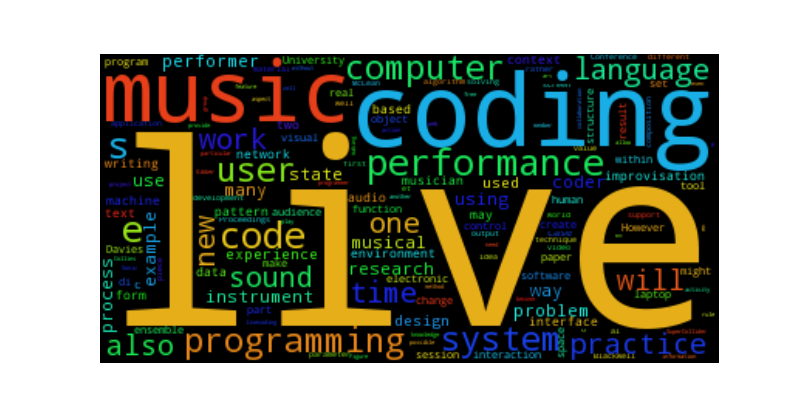
\includegraphics[scale=0.71]{./imagens/livecoding_cloud1.png}
\caption{Nuvem de palavras dos anais ICLC2015 \textbf{Fonte}: autor.}
\label{fig:nuvemlivecoding}
\end{center}
\end{figure}

\begin{table}
\caption{Tabela de classes qualitativas de termos utilizados nos anais do ICLC2015, agrupados por funções textuais.}
\small
    \begin{tabular}{ | p{1.5cm} | p{1.35cm} | p{2cm} | p{1.45cm} | p{1.45cm} | p{1.45cm} | p{1.45cm} | p{1.45cm} | p{1.25cm} |}
    \hline 
    \hline 

    \tiny \textbf{Número Qualitativo/Função} & \textbf{0} & \textbf{1}  & \textbf{2} & \textbf{3} & \textbf{4}  & \textbf{5} & \textbf{8} & \textbf{9}\\
    \hline 
    \hline 

    \tiny \textbf{Pessoas}  
    & - 
    & \tiny Collins, Blackwell, McLean, Grossi 
    & - 
    & - 
    & - 
    & -  
    & - 
    & - \\
    \hline

    \tiny \textbf{Aplicativos}
    & - 
    & \tiny SuperCollider, Gibber, SonicPi  
    & - 
    & - 
    & - 
    & -  
    & - 
    & \\
    \hline
    
    \tiny \textbf{Verbos}  
    & \tiny take, see, shared, networked, explore, made
    & \tiny make, provide, writing, solving, making
    & \tiny used
    & \tiny using, coding  
    & \tiny performer
    & - 
    & - 
    & -  \\
  \hline

     \tiny \textbf{Adjetivo ou numeral, ordinal}  
    & \tiny less, open, potential, similar, important, cognitive, virtual
    & \tiny first, real, electronic, visual, ensemble, possible, free, livecoding, aspect  
    & \tiny musical, many
    & \tiny new, one
    & - 
    & -  
    & \tiny live 
    & - \\
    \hline

    \tiny \textbf{Substantivo}  
    & \tiny Browser, point, approach, order, node, collaborative, number, source, present, community, server, framework, orchestra, digital, level, kind, type, memory, analysis, line, body, concept, technology, working, org, current, show, mean, end, processes, people, international
    & \tiny University, conference, proceedings, network, interface, environment, text, form, context, musician, space, paper, program, audience, function, change, control, human, laptop, interaction, structure, part, session, tool, result, create, object, case, algorithm, value, development, material, set, technique, parameter, idea, screen, video, application, support, composition, piece, knowledge, feature, cell, activity, art, action, information, method, web, rule, group, need, particular, project, allow, collaboration, programmer, member, play, output 
    & \tiny use, coder, process, state, example, way, software, research, problem, experience, design, improvisation, different, machine, pattern, audio
    & \tiny work, instrument
    & \tiny system, computer, user, language, time, practice, sound
    & \tiny programming
    & \tiny performance, code
    & \tiny ``live coding'', music  \\
    \hline
    \hline
   
    \end{tabular}
\label{tab:comparacao}
\end{table}

Uma breve análise da nuvem de palavras pode elucidar parte das questões-satélites. Na \autoref{tab:comparacao} filtrei parte dos resultados na nuvem de palavras por conjuntos de funções textuais -- sujeitos-humanos, sujeitos-ferramentas, verbos, adjetivos e substantivos -- e quantas vezes foram utilizados, em categorias qualitativas (0, menos usado e 9 o mais usado, sendo que 6 e 7 não apresentaram resultados). \footnote{O método de extração será explicado em um apêndice oportuno.}. 

No caso dos sujeitos-humanos, podemos ver nomes de Nick Collins e Alex McLean, praticantes responsáveis pela criação de um manifesto, em parceria com \citeonline{ward_live_2004}. Um fragmento deste manifesto será discutido no \autoref{cap:trabalhos_relacionados}. Pietro Grossi, é um personagem recentemente estudado por \citeonline{mori_pietro_2015} como um caso prematuro de \emph{live coding}, a partir do final da década de sessenta.

No caso dos sujeitos-ferramentas, destacamos o papel do \emph{SuperCollider}, já citado anteiormente, e do \emph{Gibber}\cite{roberts_gibber:_2012,wyse_viability_2014}\footnote{Disponível em \url{http://gibber.mat.ucsb.edu}}. Ambos são ambiente de programação para de síntese sonora e composição algorítmica. Um paradigma em comum destes ambientes: o procedimento de compilação de códigos conhecido como \emph{Just In Time} \cite{aycock_brief_2003}, que também será discutido no \autoref{cap:trabalhos_relacionados} como dispositivo técnico que permitiu a emancipação do \emph{livecoding}.

Os verbos fornecem informação sobre o comportamento dos improvisadores de códigos. Além da atividades como \emph{performatizar} e \emph{codificar}, é notável atividades sociais ligadas à visão, à escrita, à técnica, à lógica. Embora a Música seja a atividade proeminente do \emph{live coding}, não obtivemos resultados que retornassem, por exemplo, a palavra \emph{hearing}. Isso é significativo, e no \autoref{cap:trabalhos_relacionados}, exploro estas ações sob a ótica da Música de Processos de Steve Reich.

Já os adjetivos destacam características da prática, onde \emph{live} é a palavra-chave. Como será observado no \autoref{cap:trabalhos_relacionados}, a ação pode ocorrer em uma sala de concerto, um espaço público ou em uma casa noturna. Palavras como  \emph{electronic}, podem sugerir tanto uma música ``eletroacústica'', quanto gêneros de música para dançar. \emph{Visual} remete a uma característica tão fundamental quanto a Música. Um sem número de performances utilizam a projeção de telas de computadores como dispositivo de ``transparência''; isto é, uma ideologia de justificação do ato de improvisação. \emph{Ensemble} destaca uma a natureza de grupos. Poucas performances \emph{solo} são realizadas se comparadas às performances de \emph{duos}, \emph{trios}. 

Ainda no \autoref{cap:trabalhos_relacionados}, o \emph{live coding} se apropria da Música como Processo de Steve \citeonline{reich_music_1968} e da Música Generativa de Brian \citeonline{eno_music_1978} para justificar processos musicais com o virtuosismo de codificação\footnote{Neste trabalho criticamos esta visão. Ao que nos parece, ocorre uma confusão entre \emph{comportamentos criativos históricos} e, no caso do \emph{livecoding} emph{comportamentos criativos psicológicos}.}  

Palavras como \emph{university}, \emph{research} e \emph{technology}, e \emph{laptop} acusam não apenas uma prática artística, mas um Programa de Investigação Científica próprio. A esfera de pesquisa acadêmica permitiu ramos de desenvolvimento com linguagens de programação, cognição, inteligência artificial, semiologia, performance musical (improvisação), e mais recentemente, antropologia, conferindo à produção de \emph{live coding} espécie de autenticidade acadêmica.

\section{Sistemas Criativos, e o Universo de Conceitos}\label{sec:universo}

Uma sessão de \emph{live coding} é uma improvisação. Em seu artigo ``\emph{Music improvisation and creative systems}'', Alex \citeonline{mclean_music_2006},  articula a improvisação musical como uma atividade passível de formalização lógica. 

Este trabalho tem respaldo em outro, o artigo ``\emph{A preliminary framework for description, analysis and comparison of creative systems}'', de \citeonline{wiggins_framework_2006}. Por sua vez, define um mecanismo preliminar através do qual idéias de Margaret \citeonline{boden_creative_1990}, no livro ``The creative mind'' , são definidas formalmente.

\subsection{Sistemas Criativos}

O preceito para \emph{Universo de Conceitos} de McLean é a relação entre os \emph{Processos criativos} e \emph{Espaço conceitual} de Boden. Para Wiggins, ``Boden concebe o processo de criatividade como uma identificação e/ou localização de novos objetos conceituais em um espaço conceitual'' \cite[p.~450]{wiggins_framework_2006}\footnote{Tradução de \emph{Boden conceives the process of creativity as the identification and/or location of new conceptual objects in a conceptual space.}}.

Boden realiza duas taxonomias da criatividade. A primeira separa os comportamentos criativo em tipos H (históricos) e P (psicológicos). A segunda, separa o comportamento criativo em exploradores, e transformacionais. 

Comportamentos criativos do tipo H são aqueles tipos de conceitos historicamente novos, nunca inventados antes. Processos criativos do tipo P são os novos conceitos elaborados por uma pessoa\todo{\tiny Eu li uma parte do livro. Está no meu tablet, sem bateria e cabo para carregar. Assim que me organizar com isso, colocarei referências apropriadas.}. Por exemplo, os processos inventados em \emph{It's gonna rain} de Steve Reich, \emph{I'm sitting in a room} de Alvin Lucier ou as técnicas similares publicadas por Pauline \citeonline{oliveros_tape_1969} são comportamentos P-criativos que se tornaram H-criativos. Por outro lado consideramos, neste trabalho, os comportamentos criativos do \emph{livecoding} ainda como P-criativos. Carecem de tempo suficiente para serem considerados H-criativos.

Porém Wiggins poderia criticar ambas as visões (de Boden e a realizada no parágrafo anterior) da seguinte forma: ``pode ser possível, por exemplo, um comportamento ser P-criativo em uma sociedade, mas H-criativo em outra'' (\emph{Ibdem}, \emph{idem}). \footnote{Tradução de \emph{it would be possible, for example, for a creative behaviour to be only P-creative in one society, but H-creative in another.}}

A segunda taxonomia, que separa em comportamentos exploradores e transformacionais, lidam diretamente com o espaço conceitual. Se no primeiro caso este espaço é construído progressivamente com a elaboração de P-conceitos (o que pode ser observado em crianças), o transformacional é um comportamento que modifica o espaço conceitual existente, levando a filtrar quais são H-conceitos.

Para lidar formalmente com os Espaços Conceituais, Wiggins define ``criatividade'', ``computação criativa'', ``sistemas criativos'' e ``comportamentos criativos''. São apresentado na \autoref{tab:criatividade}

\begin{table}
\caption{Definições formais de criatividade por \citeonline[p.~451]{wiggins_framework_2006}}
\small
    \begin{tabular}{ | p{4cm} | p{11.25cm} |}
    \hline 
    \hline 

    \tiny{Criatividade} 
    & \tiny{``A performance de tarefas que, quando executados por um humano, são consideradas criativas''  \footnote{Tradução de \emph{The performance of tasks which, if performed by a human, would be deemed creative.}.}} \\
    \hline

    \tiny{Computação criativa} 
    & \tiny{``O estudo e suporte, através de meios e métodos computacionais, do comportamento exibido por sistemas naturais e artificiais, que são considerados criativos''. \footnote{Tradução de \emph{The study and support, through computational means and methods, of behaviour exhibited by natural and artificial systems, which would be deemed creative if exhibited by humans.}.}} \\
    \hline

    \tiny{Sistemas criativos} 
    & \tiny{``Uma coleção de processos, naturais ou automáticos, que são capazes de alcançarem ou simularem comportamentos que em humanos seria considerado criativo''} \\
    \hline

    \tiny{Comportamento Criativo} 
    & \tiny{``Um ou mais dos comportamentos exibidos por um sistema criativo''\footnote{Tradução de \emph{One or more of the behaviours exhibited by a creative system.}}} \\
    \hline
   
    \end{tabular}
\label{tab:criatividade}
\end{table}

Wiggins ainda define um \emph{Universo de possibilidades} no qual conceitos podem ser, em comportamentos transformacionais, contruídos para gerarem comportamentos H-criativos .

\subsection{Universo de conceitos ou de possibilidades}

\begin{citacao}
O universo, $\mathcal{U}$, é um espaço multidimensional, no qual dimensões são capazes de representar qualquer coisa, e todos os possíveis conceitos distintos correspondentes àqueles pontos em $\mathcal{U}$ (\ldots) Para tornar a proposta um espaço-tipo possível, permitirei que $\mathcal{U}$ contenha todos os conceitos abstratos, bem como os concretos, e que é possível representar os artefatos tanto completos e incompletos \cite[p.~451]{wiggins_framework_2006}.\footnote{Tradução de \emph{The universe, U, is a multidimensional space, whose dimensions are capable of representing anything, and all possible distinct concepts correspond with distinct points in U. (\ldots) To make the proposal as state-spacelike as possible, I allow that U contains all abstract concepts as well as all concrete ones, and that it is therefore possible to represent both complete and incomplete artefacts}}
\end{citacao}

Para diferenciar o Universo $\mathcal{U}$, do Espaço conceitual $\mathcal{C}$, Wiggins esclarece que Boden não reconhece de forma explícita $\mathcal{U}$, sendo que ``ela borra a distinção entre as regras que determinam a adesão do espaço (\ldots) e outras disposições que possam permitir a construção e/ou detecção de um conceito representado por um ponto no espaço'' \cite[p.~451]{wiggins_framework_2006}. Portanto, diferentes espaços conceituais estão contidos em $\mathcal{U}$;

Nas palavras de \citeonline{mclean_music_2006}, regras que validam a concepção do conceito no universo, são representadas como um conjunto$\mathcal{R}$. Regra que determinam estratégia de detecção (transversais) de um conceito no universo, são representados como o conjunto $\mathcal{T}$. Para lidar com estas regras, é necessária uma \emph{linguagem} $\mathcal{L}$ para expressá-las. Nas palavras de Wiggins: ``um conjunto de sequências compostas por algum alfabeto $\mathcal{A}$''\footnote{Tradução de \emph{it as the set of all sequences composed of some alphabet, A.}}

A \autoref{tab:universodeconceitos} ilustra os termos até agora trabalhados por McLean:

\begin{table}[!h]
\caption{Definições formais do Universo de possibilidades de \citeonline{wiggins_framework_2006}, ou Universo de Conceitos por \citeonline{mclean_music_2006}.}
\small
    \begin{tabular}{ | p{4cm} | p{5.5cm} | p{5.5cm} |}
    \hline 
    \hline 

    \tiny{Representação} 
    & \tiny{Nome}      
    & \tiny{Significado} \\
    \hline

    $c$
    & \tiny{Conceito} 
    & \tiny{Uma instância de um conceito, abstrato ou concreto \cite{wiggins_framework_2006}.} \\
    \hline

    $\mathcal{U}$
    & \tiny{Universo de Conceitos} 
    & \tiny{Superconjunto não restrito de conceitos. \cite{wiggins_framework_2006}. ``Um universo de todos conceitos possíveis'' \cite{mclean_music_2006} \footnote{Tradução de \emph{A universe of all possible concepts}.}}\\
    \hline

    $\mathcal{L}$
    & \tiny{Linguagem} 
    & \tiny{Linguagem utilizada para expressar regras.} \\
    \hline

    $\mathcal{A}$
    & \tiny{Alfabeto} 
    & \tiny{Alfabeto da linguagen que contêm caracteres apropriados} \\
    \hline

    $\mathcal{R}$
    & \tiny{Regras de validação} 
    & \tiny{Validam os conceitos em um universo, se apropriados ou não para o espaço trabalhado.} \\
    \hline

    $[[.]]$
    & \tiny{Função de interpretação} 
    & \tiny{``Uma função parcial de $\mathcal{L}$ para funções que resultam em números reais entre [0, 1] (\ldots) 0.5 $[$ou maior$]$ significa uma verdade booleana e menos que 0.5 siginifica uma falsidade booleana; a necessidade disso para valores reais se tornará clara abaixo'' \cite[p.~452]{wiggins_framework_2006}\footnote{Tradução de \emph{(\ldots) a partial function from $\mathcal{L}$ to functions yielding real numbers in [0, 1]. (\ldots) 0.5 to mean Boolean true and less than 0.5 to mean Boolean false; the need for the real values will become clear below}.}}\\
    \hline

     $[[\mathcal{R}]]$
    & \tiny{Regras de validação} 
    & \tiny{``Uma função que interpreta $\mathcal{R}$, resultando em uma função indicando aderência ao conceito em $\mathcal{R}$''\footnote{Tradução de \emph{A function interpreting $\mathcal{R}$, resulting in a function indicating adherence of a concept to $\mathcal{R}$}}} \\
    \hline

     $\mathcal{C} = [[\mathcal{R}]](\mathcal{U}) $
    & \tiny{Espaço Conceitual} 
    & \tiny{``Todos espaços conceituais são um subconjunto não-estrito de $\mathcal{U}$''\footnote{Tradução de \emph{All conceptual spaces are non-strict subset}.}. Um subconjunto contido em $\mathcal{U}$ \cite{wiggins_framework_2006}. Uma função que interpreta $\mathcal{R}$, resultando em uma função que indica aderência ao conceito em $\mathcal{R}$ \footnote{Tradução de \emph{A function interpreting $\mathcal{R}$, resulting in a function indicating adherence of a concept to $\mathcal{R}$}.} } \\
    \hline

    $\mathcal{T}$
    & \tiny{Regras de detecção} 
    & \tiny{``Regras definidas dentro de $\mathcal{L}$ para definir estratégias transversais para localizar conceitos dentro de $\mathcal{U}$'' \cite{mclean_music_2006}\footnote{Tradução de \emph{Rules defined within $\mathcal{L}$ to define a traversal strategy to locate concepts within $\mathcal{U}$ }}} \\
    \hline

    $\mathcal{E}$
    & \tiny{Regras de qualidade} 
    & \tiny{``(\ldots) conjunto de regras que permitem-nos avaliar qualquer conceito que nós encontramos em $\mathcal{C}$ e determinar sua qualidade, de acordo com critérios que nós considerarmos apropriados'' \cite[p.453]{wiggins_framework_2006}\footnote{Tradução de \emph{(\ldots) set of rules which allows us to evaluate any concept we find in C and determine its quality, according to whatever criteria we may consider appropriate.}}``Regras definidas dentro de $\mathcal{L}$ para avaliar a qualidade ou a desejabilidade do conceito $c$'' \cite{mclean_music_2006}\footnote{Tradução de \emph{Rules defined within $\mathcal{L}$ which evaluate the quality or desirability of a concept $c$.}}}\\
    \hline

    $<<<\mathcal{R}, \mathcal{T}, \mathcal{E}>>>$
    & \tiny{Função de interpretação} 
    & \tiny{Uma regra necessária para definir o espaço conceitual, ``independentemente da ordem, mas também, ficcionalmente, enumerá-los em uma ordem particular, sob o controle de $\mathcal{T}$ -- isto é cricial para a simulação de um comportamento criativo de um $\mathcal{T}$ particular \cite{wiggins_framework_2006} \footnote{Tradução de \emph{We need a means not just of defining the conceptual space, irrespective of order, but also, at least notionally, of enumerating it, in a particular order, under the control of $\mathcal{T}$ -- this is crucial to the simulation of a particular creative behaviour by a particular $\mathcal{T}$.}}. ``Uma função que interpreta a estratégia transversal $\mathcal{T}$, informada por $\mathcal{R}$ e $\mathcal{E}$ . Opera sobre um subconjunto ordenado de $mathcal{U}$ (do qual tem acesso randômico) e resulta em outro subconjunto ordenado de $\mathcal{U}$.''\footnote{Tradução de \emph{A function interpreting the traversal strategy $\mathcal{T}$, informed by $\mathcal{R}$ and $\mathcal{E}$ . It operates upon anordered subset of $mathcal{U}$ (of which it has random access) and results in another ordered subset of $\mathcal{U}$.}}} \\
    \hline
    \hline
   
    \end{tabular}
\label{tab:universodeconceitos}
\end{table}



\section{O modelo de improvisação}

TODO ...

\section{Exemplo concreto da multiplicadade em um universo de possibilidades}

Durante a pesquisa, investigamos um campo específico, mas que não será utilizado como trabalho final. Por outro lado, permitiu visualizar os conceitos  $c$ de universo de conceitos $U$ em uma mídia social (\emph{Soundcloud}).

As \autoref{fig:pacotao}, \autoref{fig:pacotao2}, ilustram a multiplicidade de conceitos $c$. Agrupados por data, país, cidade e \emph{hashtags} que ``delimitam'' um gênero musical, possibilitaram reduzir um pouco o estudo, mas não completamente.

\begin{figure}[h]
\begin{center}
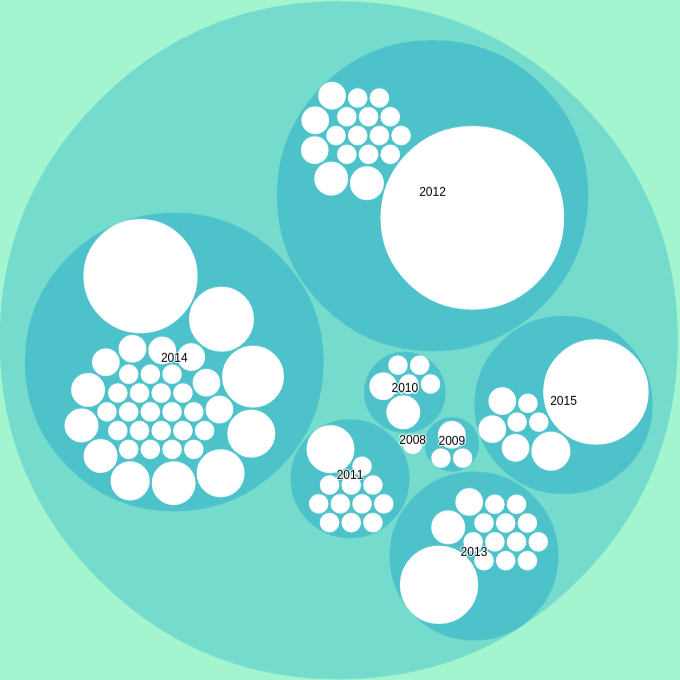
\includegraphics[scale=0.6]{./imagens/zoomable_circle_packing_genre_year_livecoding.png}
\caption{Empacotamento de informações a respeito de gênero musical a partir de anos de produção}
\label{fig:pacotao}
\end{center}
\end{figure}

Os seguintes os termos delimitados foram: \begin{inparaenum}[\itshape a)\upshape]
\item \emph{livecoding}/\emph{live-coding}: dados coerentes com a bibliografia pesquisada\footnote{A exclusão do termo \emph{live code/live coding} foi feita pois a separação criava uma ambiguidade de busca no \emph{Soundcloud}, isto é, \emph{live} poderia não se referir ao que pesquisamos por \emph{livecoding}.};
\item \emph{algorave}/\emph{algopop}: parte considerável da produção do \emph{livecoding} realizada em ambientes noturnos, informais ou de entretenimento (possue relação com o elemento dança);
\item \emph{bytebeat}: parte considerável de uma técnica de programação musical descrita pela primeira vez por \citeonline{heikkila_discovering_2011} e aplicada no \emph{livecoding}, isto é, apenas um fragmento dessa prodção pode se encaixar como \emph{livecoding} (um desses programas é o \emph{Wavepot});
\item \emph{algorithmic music}:música algorítmica, seguindo a subdivisão Música Gerada por Computador, ou \emph{Computer Generated Music}\cite{cope_prefacio_2008}.
\end{inparaenum}

\begin{figure}[h]
\begin{center}
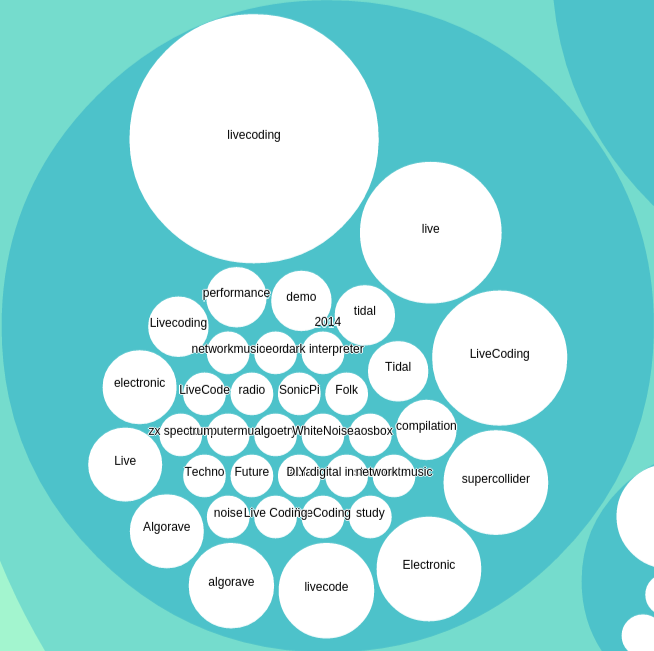
\includegraphics[scale=0.6]{./imagens/zoomable_circle_packing_genre_year_livecoding2.png}
\caption{Detalhamento de informações a respeito de gênero musical a partir de anos de produção}
\label{fig:pacotao2}
\end{center}
\end{figure}

Os dados levantados são de janeiro e fevereiro de 2015; não realizamos mais levantamentos. Os motivos foram: \begin{inparaenum}[\itshape i)\upshape]
\item a dificuldade de análise das assimetrias observadas, que requerem maior experiência com técnicas estatísticas.
\item os dados ilustram as variedades de categorizações musicais no \emph{live coding}. Pode ser interessante observar se tais variedades se aplicam em um único \emph{live coder}.
\end{inparaenum}

\begin{figure}
\begin{center}
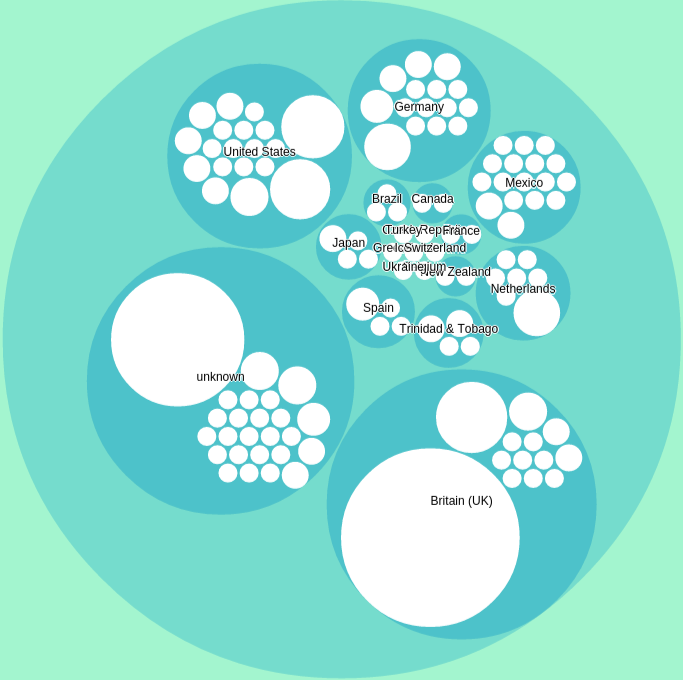
\includegraphics[scale=0.6]{./imagens/zoomable_circle_packing_genre_year_livecoding3.png}
\caption{Empacotamento de informações a respeito de gênero musical a partir de países onde ocorreram as produções}
\label{fig:pacotao3}
\end{center}
\end{figure}

Antes de discutir três casos específicos de um \emph{live coder} (Sorensen), contextualizamos os \emph{live coding} no \autoref{cap:trabalhos_relacionados}. Alguns precedentes históricos do \emph{live coding}, como \emph{GROOVE}, o compositor \emph{Pietro Grossi}, a \emph{Live Computer Music} da Baía de São Franscisco entre os anos 70 e 80 nos Estados Unidos, e a emancipação de uma organização, TOPLAP\footnote{Disponível em \url{http://www.toplap.org}.}, e o destaque de \emph{live coders} ingleses, foram fatores para descrever, neste trabalho, o \emph{live coding} como técnica de improvisação artística original de um Norte político e econômico; delimitar o \emph{live coding} como um Programa de Investigação Científica em universidades; ou descrever o \emph{live coding} como dispositivo de improvisação para replicação de categorizações musicais.

\begin{figure}
\begin{center}
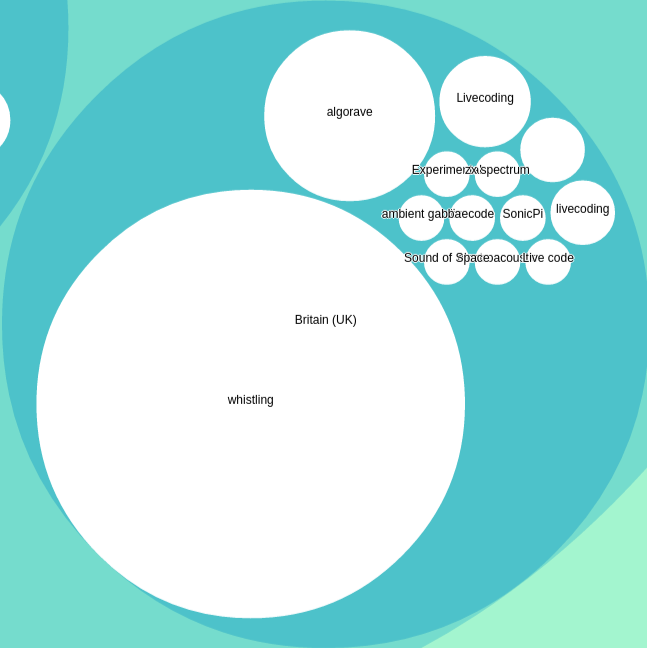
\includegraphics[scale=0.6]{./imagens/zoomable_circle_packing_genre_year_livecoding4.png}
\caption{Detalhamento de informações a respeito de gênero musical a partir de países onde ocorreram as produções.}
\label{fig:pacotao4}
\end{center}
\end{figure}
\newpage
\chapter{Metodologia de análise de uma Improvisação musical de códigos}\label{cap:metodologia}

Este capítulo contextualiza a \emph{criatividade} dentro do pensamento proposto por um improvisador programador \cite{McLean2011. Apresentaremos uma definição de criatividade \ver{sec:diferencas} para contextualizar o \traducao{Quadro Conceitual de Sistemas Criativos}{Creative System Frameworks} \ver{sec:csf}. Este quadro é uma interessante ferramenta teórica para análise formal de improvisações. Em seguida formalizamos este quadro para os propósitos específicos desta pesquisa.

\section{O paradoxo da criatividade}\label{sec:diferencas}

Para definir \emph{criatividade} com o propósito de analisar uma improvisação de códigos, seguiremos a proposição do livro ``The Creative Mind: myths and mechanisms'' de Margaret \citeonline{boden_creative_1990}. Segundo \citeonline[p.~2]{thornton_quantitative_2007}, a proposição de Boden apresenta um paradoxo da definição de criatividade:

\begin{citacao}
\traducao{O ponto inicial de Boden para o desenvolvimento de sua sua explicação, é a observação de que o conceito de criatividade contém um paradoxo. Por definição, criatividade cria, i.e., produz alguma coisa nova. Mas se estamos comprometidos com uma abordagem mecanicista do mundo -- nenhum milagre é permitido -- iremos acreditar que tudo o que ocorre é, em princípio, previsível. Iremos acreditar também que qualquer coisa nova deve ser construída de componentes existentes. Isso implica que nada pode ser intrinsicamente novo.}{Boden’s starting point for the development of her account is the observation that the concept of creativity contains a paradox. By definition, creativity creates, i.e., it produces something new. But if we are committed to a mechanistic account of the world — no miracles allowed — we believe that everything that occurs is predictable in principle. We also believe that any new thing must be constructed from existing components. This implies that nothing can ever be intrinsically new.}
\end{citacao}

O comportamento criativo, é socialmente avaliado por sua capacidade de gerar \emph{novidades}. De outro ponto de vista, o mecanismo de julgamento do que é ou não é novidade parte de uma identificação do que é possível e do que não é, de forma que a impossibilidade é valorizada: \traducao{Para justificar a classificação de uma idéia criativa... alguém deve identificar os princípios generativos com respeito ao que é impossível}{To justify calling an idea creative... one must identify the generative principles with respect to which it is impossible.} \apud[p.~40;p.~3]{boden_creative_1990}{thornton_quantitative_2007}. Veremos que essa capacidade gerativa do aparentemente impossível está conectada com uma restrição daquilo que já existe. A restrição de regras, a utilização de uma linguagem para representar as regras, e a aplicação de estratégias transversais que possibilitam a praticidade das restrições \ver{sec:csf}. Isso inverte a idéia comum de criatividade:  \traducao{Qualquer ato criativo é fundado na conceitualização ou realização de um ponto dentro de um espaço conceitual particular (\emph{idem}, \emph{ibidem})}{Any creative act is thus founded on conceptualisation or the realisation of a point within a particular ‘conceptual space’.}.

Para Thornton e \citeonline[p.~450--451]{wiggins_framework_2006}, na primeira edição doeseu livro, Boden não explica como é o método de acesso aos espaços conceituais. Por outro lado, Boden oferece uma taxonomia de tipos de criativadade. As nomenclaturas derivadas são explicadas como uma divisão de duas classificações da criatividade \ver{fig:ortogonal}. A primeira classificação divide a criatividade em criatividade-psicológica, ou criatividade-pessoal (\emph{P-creativity}), e criatividade-histórica (\emph{H-creativity}). A segunda classificação separa criatividade em criatividade-exploradora e criatividade-transformacional.

\begin{figure}
\centering
\begin{tikzpicture}[scale=2.5]
\tikzstyle{every node}=[draw,shape=circle];
\path (0:0cm) node (v0) {\tiny $Criatividade$};
\path (0:1.25cm) node (v1) {\tiny $Criatividade-H$};
\path (2*90:1.25cm) node (v2) {\tiny $Criatividade-P$};
\path (3*90:1.25cm) node (v3) {\tiny $Criatividade Exp.$};
\path (90:1.25cm) node (v4) {\tiny $Criatividade Trans.$};
\draw (v0) -- (v1)
(v0) -- (v2)
(v0) -- (v3)
(v0) -- (v4);
\end{tikzpicture}
\caption{Classificação da criatividade : 1) criatividade-psicológica/criatividade-histórica; 2) critividade exploradora/criatividade transformacional. \textbf{Fonte}: autor com base em \citeonline{wiggins_framework_2006}.}
\label{fig:ortogonal}
\end{figure}

\begin{citacao}
\traducao{A distinção é entre o sentido de criar um conceito que nunca foi criado antes $[$criatividade-P$]$, e um conceito que nunca foi criado antes por um criador específico $[$criatividade-H$]$. Esta distinção será tangencialmente relevante para meu argumento aqui, mas antes de prosseguir, eu noto que esta não é uma simples escolha binária, mas ao invés, uma contextualização multidimensional: pode ser possível, por exemplo, para um comportamento criativo ser P-criativo em uma sociedade, mas H-criativo em outra; deste ponto de vista da segunda sociedade, apenas importam comportamentos H-criativos. (\ldots) no trabalho de Boden, existe uma distinção entre criatividade exploradora e transformacional, que será relevante aqui, e então merece alguma explicação. Boden concebe o processo de criatividade como uma identificação e/ou localização de novos objetos conceituais em um espaço conceitual.}{The distinction is between the sense of creating a concept which has never been created before at all, and a concept which has never been created before by a specific creator. This distinction will be only tangentially relevant to my argument here, but before proceeding, I note that this is not a simple binary choice, but rather multi-dimensional, context-based one: it would be possible, for example, for a creative behaviour to be only P-creative in one society, but H-creative in another; from the point of view of the second society, only the H-creativity matters. (\ldots) in Boden’s work, there is the distinction between exploratory and transformational creativity, which is directly relevant here, and so needs a little more explanation. \textbf{Boden conceives the process of creativity as the identification and/or location of new conceptual objects in a conceptual space}.}  
\end{citacao}

Para Wiggins, Boden chama de \emph{comportamento criativo explorador} a exploração de possibilidades completas ou parciais de um conceito. Já o \emph{comportamento criativo transformacional} pressupõe regras governadoras deste espaço conceitual em exploração, e busca transformar tais regras através de métodos. Para Boden,  são socialmente valorizados os conceitos-H e os processos transformacionais, enquanto o comportamento explorador e a criatividade-P são consideradas como característicos de crianças mais novas, ou pensamentos personalistas. Wiggins dá maior importância para a classificação exploradora/transformacional, e não desvaloriza o comportamento explorador em relação à transformação..  \citeonline[p.~3--4]{thornton_quantitative_2007} pontua que Boden admite que em algumas situações, uma criativade-exploradora não é menos criativa que uma criativade-transformadora. O comportamento explorador, como uma \emph{exploração guiada}, é muito útil em atividades onde se requer \traducao{(\ldots) a utilização de heurísticas e mapas para identificar conceitos valiosos dentre de um espaço conceitual existente}{the use of heuristics and maps to identify valuable concepts within an existing conceptual space} \ver{sec:showusyourscreens}. Neste sentido, os comportamentos criativos \emph{apenas transformadores} desenvolvem novos espaços conceituais que serão úteis para o comportamento explorador guiado. 

\begin{citacao}
\traducao{De fato, na primeira edição $[$\citeonline{boden_creative_1990}$]$, ela não oferece uma explicação do número de diferentes tipos de criatividade que ela identificou. Parece que sua intenção era distinguir os dois tipos notados, espaços conceituais devem ter uma característica generativa. E isso certamente é a interpretação comum. Ainda no sumário 'em uma casca de noz' de sua teoria, foi adicionado um prólogo à segunda edição (Boden, 2003), e em (Boden, 1998), ela coloca que sua explicação distingue três principais formas de criatividade, sendo exploração, transformação e \emph{combinação}. É somada à incerteza a observação que somente a definição forte $[$generalizadora$]$ da definição possue o poder de resolver o paradoxo da criatividade}{In fact, in the first edition, she offers no final count of the number of different types of creativity she has identified. It seems to be her intention to distinguish the two types noted, conceptual space must be generative in character. and this is certainly a common interpretation. Yet in the ‘nutshell’ summary of her theory, added as a prologue to the second edition (Boden, 2003), and in (Boden, 1998), she states that her account distinguishes three main forms of creativity, these being exploration, transformation and combination. Adding to the uncertainty is the observation that only the strong definition has the power to resolve the creativity paradox, arguably forcing us to recognise not two forms of creativity, or three, but one: transformation.}
\end{citacao}

Neste ponto \citeonline[p.~451]{wiggins_framework_2006} apresenta uma definição cíclica e generalizadora de criatividade, \traducao{A performance de tarefas que, quando executados por um humano, são consideradas criativas}{The performance of tasks which, if performed by a human, would be deemed creative}, e subdivide em quatro definições auxiliares: 

\begin{table}[!h]
\caption{Definições formais de criatividade por \citeonline[p.~451]{wiggins_framework_2006}}
\small
    \begin{tabular}{ | p{4cm} | p{11.25cm} |}
    \hline 
    \hline 

    \tiny{Criatividade} 
    & \tiny{``O estudo e suporte, através de meios e métodos computacionais, do comportamento exibido por sistemas naturais e artificiais, que podem ser considerados criativos se exibidos em humanos.''  \tablefootnote{Tradução de \emph{‘The study and support, through computational means and methods, of behaviour exhibited by natural and artificial systems, which would be deemed creative if exhibited by humans’’.}.}} \\
    \hline

    \tiny{Computação criativa} 
    & \tiny{``O estudo e suporte, através de meios e métodos computacionais, do comportamento exibido por sistemas naturais e artificiais, que são considerados criativos''. \tablefootnote{Tradução de \emph{The study and support, through computational means and methods, of behaviour exhibited by natural and artificial systems, which would be deemed creative if exhibited by humans.}.}} \\
    \hline

    \tiny{Sistemas criativos} 
    & \tiny{``Uma coleção de processos, naturais ou automáticos, que são capazes de alcançarem ou simularem comportamentos que em humanos seriam considerados criativos''} \\
    \hline

    \tiny{Comportamento Criativo} 
    & \tiny{``Um ou mais dos comportamentos exibidos por um sistema criativo''\tablefootnote{Tradução de \emph{One or more of the behaviours exhibited by a creative system.}}} \\
    \hline
    \hline
   
    \end{tabular}
\label{tab:criatividade}
\end{table}

\subsection{Criatividade, códigos e imagens mentais}\label{sec:imagem_mental}

Para \citeonline[p.~24--25]{McLean2011}, um comportamento criativo pode ser descrito como o processo de elaboração de uma \emph{imagem mental}. Mais especificamente, a imagem mental é um símbolo, e seu significado é governado por regras gramaticais e sociais (códigos). Por outro lado, McLean estabelece o conceito de \emph{imagem mental} como uma hierarquia de códigos simbólicos, visuais e gramaticais, como descrita pela teoria da Codificação Dual \apud[p.~25--29]{paivio_dual_1990}{McLean2011}:


\begin{citacao}
\traducao{Seu $[$Paivio$]$ argumento não é que existem dois códigos, mas sim que existe uma hierarquia de códigos, que se ramificam no topo em códigos lingüísticos discretos e códigos de percepção contínua, que Paivio nomeia como \emph {logogens} e \emph{imagens} respectivamente. (\ldots) \textbf{A explicação oferecida pela teoria da Codificação Dual é que existem sistemas de símbolos distindos, mas integrados, para linguagens e figuras}.}{His contention is not that there are two codes, but rather that there is a hierarchy of code, which branch at the top into discrete linguistic codes and contionuous perceptual codes, which Paivio names \emph{logogens} and \emph{imagens} respectively (\ldots) The explanation offered by Dual Coding Theory is that there are distinct, yet integrated symbol systems for imagery and language.}
\end{citacao}

Por exemplo, quando falamos em \emph{improvisação de códigos}, podemos imaginar uma pessoa escrevendo um texto em um computador. Dependendo do grau de intimidade com os símbolos aprendidos, pode ser que esta imagem seja mais ou menos específica, e , outras possibilidades de imagens mentais surgem. A própria atividade de descrição de uma imagem mental é uma \emph{estratégia} de conversão. No caso do improvisador-programador, que converte sua imagem mental em em código de computador, chamaremos de \emph{estratégia transversal}.

Neste processo, o improvisador-programador recorre aos padrões e estilos de escrita de uma linguagem. Entre padrões e estilos, são utilizados comentários, que explicam textualmente a imagem e seu resultado; da disposição espacial do código, ou  nomes de variáveis e funções que sugerem imagens mentais específicas. No caso de uma linguagem de programação de propósito geral, algumas regras definidas pela comunidade desenvolvedora da linguagem devem ser seguidas. No entanto, já vimos que o improvisador-programador é estimulado a recorrer às linguagens artificiais, ou linguagens de domínio específico (DSL) -- ``O programa será transcendido - Língua Artificial é o caminho'' \ver{sec:showusyourscreens}. Isto é, é parte da prática do improvisador-programador criar linguagens específicas para uma classe de imagens mentais específicas. 

Um exemplo de exploração de um processo transformacional será ilustrado a partir de uma descrição de \citeonline[p.~119]{McLean2011},  com o método da \emph{prática reflexiva} de um artista-plástico (no caso, o pintor Paul Klee). Supondo a discretização do processo transformacional, o artista cria uma imagem mental do que irá fazer, um esboço que delimita um campo de atividade (espaço conceitual), a atividade de pintura, e o resultado percebido.  Na fase de implementação do esboço, o pintor percebe que aquilo que foi considerado adequado no esboço, é inadequado para a situação prática. Neste momento, o artista reage ao resultado e re-elabora novas estratégias de conversão entre a imagem mental e o resultado. O processo continua até que o ofício seja considerado completo (\emph{obra}). Este não é o mesmo processo utilizado pelo(a) improvisador(a)-programador(a). O material, e o objetivo são diversos do(a) artista plástico(a). Seu material é o texto, mas não o texto discursivo, e sim o texto que descreve uma rotina de tarefas computacionais. Seu objetivo não é chegar a uma obra finalizada, mas sim não descontinuar o processo. McLean chama esse método de transformacional de programação por bricolagem \ver{fig:processo_criativo}. Em ambos os casos, na prática reflexiva e na bricolagem, são necessários conceitos que suportem a intenção (e vontade) do ofício. Conceitos elaborados através de restrições de idéias podem ser sistematizados, com o auxílio de esquemas visuais. Esta abordagem é muito semelhante à posição defendida por McLean, onde conceitos podem ser representados geometricamente. No caso do(a) improvisador(a)-programador(a), \emph{espaços conceituais} são reelaborados indefinidamente, começando por uma \emph{estratégia transversal}, passando para a observação, reação, e reformulação da imagem mental.

 \begin{figure}[h]
  \centering
  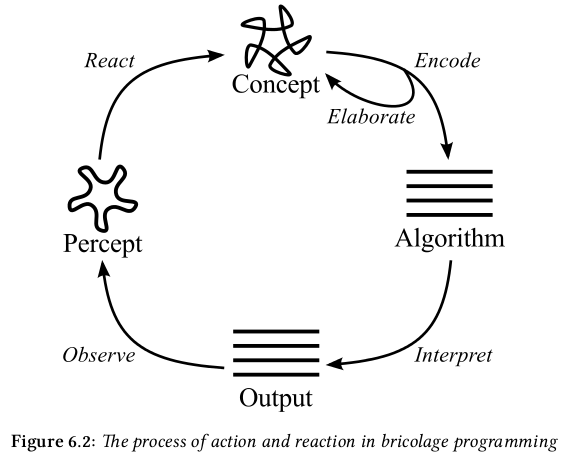
\includegraphics[scale=0.5]{imagens/processo_criativo.png}
  \caption{Modelo de bricolagem para o processo criativo realizado por um artista-programador. \textbf{Fonte}: \citeonline[p.~122]{McLean2011}. }
  \label{fig:processo_criativo}
\end{figure}

\begin{citacao}
\traducao{A Figura 6.2 $[$\autoref{fig:processo_criativo}$]$ caracteriza a programação por bricolagem como um laço retroalimentado envolvendo o algoritmo escrito, sua interpretação, e a percepção do programador e sua reação do resultado ou comportamento $[$do algoritmo$]$. (\ldots). No começo o programador tem um conceito meio-formado que só atinge consistência interna através do processo de ser expresso como um algoritmo. O laço interno é onde o programador elabora o objetivo de suas imaginações, e o laço externo é onde essa trajetória está fundamentada na pragmática do que elas realmente têm que fazer. Através deste processo ambos algoritmos e conceitos são desenvolvidos até que o programador sinta que um se aplica com o outro, ou de outra forma julga o processo criativo finalizado.
}{
Figure 6.2 characterises bricolage programming as a creative feedback loop encompassing the written algorithm, its interpretation, and the programmer’s perception and reaction to its output or behaviour. (\ldots). At the beginning, the programmer may have a half-formed concept, which only reaches internal consistency through the process of being expressed as an algorithm. The inner loop is where the programmer elaborates upon their imagination of what might be, and the outer where this trajectory is grounded in the pragmatics of what they have actually made. Through this process both algorithm and concept are developed, until the programmer feels they accord with one another, or otherwise judges the creative process to be finished.
}  
\end{citacao}

 Para McLean, DSLs ``provêm termos padronizados para descrever demandas particulares em um domínio de uma tarefa''. Isto é, uma linguagem customizada para atividades artísticas pode ser planejada, ou analizada, através de um \emph{Quadro de estruturação das Dimensões Cognitivas da Notação} \apud[p.~95--97]{church_cognitive_2008}{McLean2011}. Estas não são dimensões autônomas, o que diverge do foco de nosso trabalho. Uma situação comum na improvisação de códigos, é maleabilidade de escrita de um algoritmo. No caso, McLean define como a interdependência entre viscosidade e notação secundária: a possibilidade de diferentes soluções para o mesmo resultado. Por exemplo, em um \emph{patch} de PD, cuja imagem mental é uma onda quadrada. Podemos utilizar objetos nativos ou objetos extendidos \ver{fig:pd}. Uma outra interdependência de dimensões, entre as Operações Mentais Difíceis e a não-Invisibilidade de Dependências Escondidas, é notória do ponto de vista pedagógico. Podem afastar o compositor de seu objetivo musical, mais ou menos estruturado em uma teoria. DSLs como PureData, Max/MSP, CSound, SuperCollider, Tidal, praticam a invisibilidade de dependências em diferentes graus. Porém, entre os improvisadores de código, é considerado virtuosismo o praticante recorrer às Operações Mentais difíceis com o mínimo possível de Invisibilidade de Dependências. Por exemplo, utilizar linguagens de baixo nível como C \ver{sec:concerto}, ou de alto nível como Perl \cite{mclean_hacking_2004} e ainda assim, elaborar sons e imagens de maneira criativa. \ver{tab:dimensoes}:

\begin{table}[!h]
\caption{Dimensões cognitivas da Notação para linguagens de programação. \textbf{Fonte}: \apud{church_cognitive_2008}{McLean2011}.}
\small
    \begin{tabular}{ | p{7cm}| p{7cm} |}
    \hline 
    \hline 

    \tiny \textbf{Dimensão} & \textbf{Significado} \\
    \hline 
    \hline 

    \tiny \textbf{Abstração}  
    & \tiny \tabletraducao{Disponibilidade de mecanismos de abstração}{Avaliability of abstraction mechanisms} \\
    \hline

    \tiny \textbf{Dependências escondidas}

    & \tiny \tabletraducao{Invisibilidade de ligações importantes entre entidades.}{Invisibility of important links between entities.}\\
    \hline
    
    \tiny \textbf{Compromisso prematuro}  
    & \tiny \tabletraducao{Restrição na ordem de execução das coisas.}{Constraints on the order of doing things.} \\
  \hline

    \tiny \textbf{Notação secundária}  
    & \tiny \tabletraducao{Notação diversa da sintaxe formal.}{Notation other than formal syntax.} \\
    \hline

    \tiny \textbf{Viscosidade}  
    & \tiny \tabletraducao{Resistência à mudança.}{Resistance to change.} \\
    \hline

    \tiny \textbf{Proximidade de mapeamento}  
    & \tiny \tabletraducao{Proximidade de representação para o domínio-alvo.}{Closeness of representation to target domain.} \\
    \hline

    \tiny \textbf{Consistência}  
    & \tiny \tabletraducao{Semânticas similares são expressadas em formas sintáticas similares.}{Similar semantics are expressed in similar syntatic forms} \\
    \hline

    \tiny \textbf{Dispersividade}  
    & \tiny \tabletraducao{Prolixidade da linguagem.}{Verbosity of language.} \\
    \hline

    \tiny \textbf{Tendência ao erro}  
    & \tiny \tabletraducao{Probabilidade de erros.}{Likelihood of mistakes.} \\
    \hline

    \tiny \textbf{Operações mentais difíceis}  
    & \tiny \tabletraducao{Demanda de recursos cognitivos.}{Demand on cognitive resources.} \\
    \hline

    \tiny \textbf{Provisoriedade}  
    & \tiny \tabletraducao{Grau de compromisso com ações e marcos.}{Degree of commitment to actions or marks.} \\
    \hline
    
    \tiny \textbf{Função de expressividade}  
    & \tiny \tabletraducao{medida em que o efeito de um componente pode ser inferida.}{Extent to which the purpose of a component may be inferred.} \\
    \hline
    \hline
   
    \end{tabular}
\label{tab:dimensoes}
\end{table} 

\begin{figure}[!h]
  \centering
  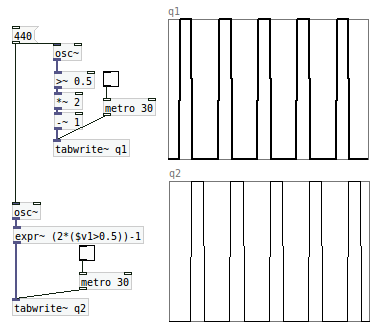
\includegraphics[scale=0.7]{imagens/pd.png}
  \caption{Exemplo de uma caracteristica de viscosidade e notação secundária no PureData. \textbf{Fonte}: autor. }
  \label{fig:pd}
\end{figure}

 
\subsection{Comportamento Criativo: Bricolagem como estratégia transversal}\label{sec:tidal}

Vamos ilustrar um pequeno processo da \emph{estratégia transversal} com o \emph{software} Tidal.
Segundo \citeonline[p.~2]{mclean_tidal_2010}, \emph{Tidal} é uma linguagem de composição generativa, onde \traducao{padrões podem ser compostos de numerosos subpadrões em uma variedade de maneiras e para uma profundidade arbitrária, para produzir $[$partes$]$ inteiras complexas de partes simples}{patterns may be composed of numerous subpatterns in a variety of ways and to arbitrary depth, to produce complex wholes from simple parts}. Amostras sonoras representam imagens mentais de suas fontes (por exemplo ``sn'' para \emph{snare}, caixa-clara), com ritmos organizados com o auxílio de símbolos delimitadores de tempo (como espaço, `` ``, e colchetes, ``$[$'',``$]$'', \verb|{| e \verb|}|). Ritmos podem ser revertidos (\verb|rev|), diminuidos e aumentados (\verb|slow|, \verb|density|), iterados (\verb|every|) para recombinação permutação, padrões mais complexos (\verb|can|), como o algoritmode bjorklund que simula ritmos tradicionais\footnote{\cfcite{toussaint_euclidean_2005}}. Efeitos de panoramização, atraso (\emph{delay}), filtros e comunicação de rede. No Exemplo \ref{ex:tidal}. a imagem mental é a demanda da linguagem, que é produzir Música Eletrônica para Dançar.

\begin{citacao}
\traducao{Tidal é uma linguagem de padrões embebida em uma linguagem de programação Haskell, consistindo de representação de padrão, uma biblioteca de padrões geradores e combinadores, um $[$mecanismo$]$ de agendamento de eventos e uma interface para programar ao vivo. Esta é uma extensiva re-escrita de um trabalho anterior introduzido sobre o título \emph{Petrol} $[$\citeonline{mclean_petrol_2010}$]$. Extensões incluem melhoramentos de representação de padrão e um uma integração totalmente configurável do protocolo Open Sound Control $[$\citeonline{osc}$]$ \cite{mclean_tidal_2010}
}
{Tidal is a pattern language embedded in the Haskell programminglanguage, consisting of pattern representation, a library of pattern generators and combinators, an event scheduler and programmer’s live coding interface. This is an extensive re-write of earlier work introduced under the working title of Petrol [15]. Extensions include improved pattern representation and fully configurable integration with the Open Sound Control (OSC) protocol [16]
}
\end{citacao}

\begin{example}{Exemplo de Estratégia Transversal}\label{ex:tidal}

Imagem mental: um \emph{loop} sincopado, mas bastante regular, descrito em um compasso. Em uma ``partitura-mental'', estruturamos o primeiro tempo com um baixo, que volta a tocar na segunda semicolcheia do terceiro tempo. No Segundo tempo, silêncio. No quarto tempo uma caixa aberta:

{%
\parindent 0pt
\noindent
\ifx\preLilyPondExample \undefined
\else
  \expandafter\preLilyPondExample
\fi
\def\lilypondbook{}%

\includegraphics{53/lily-86c766d2-1}%
% eof

\ifx\postLilyPondExample \undefined
\else
  \expandafter\postLilyPondExample
\fi
}

O padrão acima pode ser elaborado em uma voz (\verb|d1|), que redireciona (\$) a função que toca amostras sonoras (\verb|sound|). Esta função lê uma corrente de caracteres (\textbf{string}) separados por um espaço em branco. Espaços em branco são delimitadores temporais. Cada subdivisão temporal é representada por delimitadores como $[$ e $]$. 

\begin{minted}{haskell}
-- Eletronic Dance Music, BPM = 120 
-- tempo 1 - baixo            (bass)
-- tempo 2 - silencio         (silence)
-- tempo 3 - silencio + baixo
-- tempo 4 - caixa            (sn e sn:4)
d1 \$ (sound "bass3 silence [silence bass3] sn:4")
\end{minted}

Sonoramente, é útil para começar. Mas uma Música Eletrônica para Dançar requer mais elementos. Seguiremos com mais dois passos. Podemos complementar os ritmos com uma caixa e um baixos mais secos no segundo e terceiro tempo.

{%
\parindent 0pt
\noindent
\ifx\preLilyPondExample \undefined
\else
  \expandafter\preLilyPondExample
\fi
\def\lilypondbook{}%

\includegraphics{c7/lily-46fd6313-1}%
% eof

\ifx\postLilyPondExample \undefined
\else
  \expandafter\postLilyPondExample
\fi
}

\begin{minted}{haskell}
-- Eletronic Dance Music, BPM = 120 
-- tempo 1 - baixo            (bass)
-- tempo 2 - silencio         (silence)
-- tempo 3 - silencio + house
-- tempo 4 - caixa            (sn e sn:4)
d1 \$ (sound "bass3 sn [silence house] sn:4")
\end{minted}

É possível também fazer com que este padrão reduza seu tempo pela metade a cada quatro tempos, :

{%
\parindent 0pt
\noindent
\ifx\preLilyPondExample \undefined
\else
  \expandafter\preLilyPondExample
\fi
\def\lilypondbook{}%

\includegraphics{2b/lily-de0a8ae3-1}%
% eof

\ifx\postLilyPondExample \undefined
\else
  \expandafter\postLilyPondExample
\fi
}

\begin{minted}{haskell}
-- Eletronic Dance Music, BPM = 120
-- com uma caixa seca no segundo tempo
-- e uma caixa aberta no quarto tempo
-- A cada 4 tempos, o ritmo diminui pela metade 
-- e depois volta ao normal.
d1 \$ every 4 (density 0.5) (sound "bass3 sn [silence house] sn:4")
\end{minted}
\end{example}

Para \citeonline[p.~130]{McLean2011}, esta estratégia criativa, de programar ``no momento'', a partir de um arquivo de texto em branco, com uma imagem mental do resultado sonoro (ou visual), é caracterizada pela  bricolagem. No início do exemplo acima, o programador elabora um meio-conceito do que quer fazer, cuja expressão apenas ganha existência através da codificação \ver{fig:processo_criativo}. As fases de observação, e reação levam o improvisador programador à reconceitualização, e um novo código é escrito. No entanto, ao invés de finalizar, o improvisador segue desenvolvendo.

\section{Quadro Conceitual de sistemas criativos}\label{sec:csf}

Uma maneira adequada de descrever um sistema criativo (ou parte dele) considera um \emph{Universo de Conceitos}:

\begin{citacao}
O universo, $\mathcal{U}$, é um espaço multidimensional, no qual dimensões são capazes de representar qualquer coisa, e todos os possíveis conceitos distintos correspondentes àqueles pontos em $\mathcal{U}$ (\ldots) Para tornar a proposta um espaço-tipo possível, permitirei que $\mathcal{U}$ contenha todos os conceitos abstratos, bem como os concretos, e que é possível representar os artefatos tanto completos e incompletos \cite[p.~451]{wiggins_framework_2006}.\footnote{Tradução de \emph{The universe, U, is a multidimensional space, whose dimensions are capable of representing anything, and all possible distinct concepts correspond with distinct points in U. (\ldots) To make the proposal as state-spacelike as possible, I allow that U contains all abstract concepts as well as all concrete ones, and that it is therefore possible to represent both complete and incomplete artefacts}}
\end{citacao}

Wiggins esclarece que Boden não reconhece de forma explícita $\mathcal{U}$, ``ela borra a distinção entre as regras que determinam a adesão do espaço (\ldots) e outras disposições que possam permitir a construção e/ou detecção de um conceito representado por um ponto no espaço'' (\emph{Idem, ibdem}). Espaços conceituais $\mathcal{C}$, finitos ou infinitos são definidos como restrições de um universo $\mathcal{U}$, caracterizando um conjunto não-determinístico de conhecimentos, representações, e conceitos:

\begin{citacao}
\traducao{A noção-chave na teoria de Boden é aquele do espaço conceitual. Enquanto nenhuma definição formal é provida, é comum interpretar esta frase literalmente, tomando o espaço conceitual sendo um espaço de conceitualizações, ou representações de conceitos \cite[p~.7]{thornton_quantitative_2007}.}{The key notion in Boden’s theory is that of the conceptual space. While no formal definition has been provided, it is common to interpret the phrase literally, taking the conceptual space to be a space of conceptualisations or concept representations.}
\end{citacao}

\citeonline[p.~452]{wiggins_framework_2006} considera  \traducao{(\ldots) um universo, $\mathcal{U}$, um espaço multidimensional, cujas dimensões são capazes de representar qualquer coisa, e todos possíveis conceitos distintos correspondentes com distintos pontos em $\mathcal{U}$.}{The universe, U, is a multidimensional space,whose dimensions are capable of representing anything, and all possible distinct concepts correspond with distinct points in U}. Uma incomensurabilidade é evitada através de uma restrição por meio de quatro axiomas. O primeiro axioma (Universalidade) estabelece que o universo $\mathcal{U}$ pode conter tantos conceitos bem definidos (completos), parcialmente definidos (incompletos), e  o mais incompleto dos conceitos. Os dois primeiros são representados pela letra $c$, enquanto o último é representado por \small{T}. O segundo axioma (Não-identidade dos conceitos), estabelece que dois conceitos em  $\mathcal{U}$ são mutuamente diferentes entre si ($c_1 \neq c_2$), e não são um Universo. Esta correção restringe a recursividade de conceitos, o que daria ênfase ao comportamento explorador e anularia a importância do comportamento transformacional. O terceiro axioma (Inclusão Universal 1) define que \emph{espaços conceituais} $\mathcal{C}$, que contêm instâncias de conceitos $c$, são subconjuntos não-estritos do conunto $\mathcal{U}$. O quarto axioma (Inclusão Universal 2) estabelece que espaços conceituais $\mathcal{C}$ também contem o conceito \small{T}.






 Wiggins define o Universo de Conceitos (\csf{U}{x}) como um conjunto não estrito dos \emph{Espaços Conceituais} (\csf{C}{x}) de Margaret \citeonline{boden_creative_1990}. Isto é, um Universo de Conceitos a respeito de alguma coisa, no nosso caso da improvisação de códigos \ver{eq:ul}. 

\begin{equation}
\mathcal{U}_\emph{livecoding} = [\mathcal{C}_\emph{Tecelagem}, \mathcal{C}_\emph{Audiovisual}, \mathcal{C}_\emph{Dança} \mathcal{C}_\emph{Música}, \ldots, ?]
\end{equation}\label{eq:ul}

\begin{table}[!h]
\caption{Definições formais do Universo de possibilidades de \citeonline{wiggins_framework_2006}, ou Universo de Conceitos por \citeonline{mclean_music_2006}.}
\small
    \begin{tabular}{ | p{4.25cm} | p{5.25cm} | p{5.25cm} |}
    \hline 
    \hline 

    Representação
    & \tiny{Nome}     
    & \tiny{Significado} \\
    \hline

    $c$
    & \tiny{Conceito} 
    & \tiny{Uma instância de um conceito, abstrato ou concreto \cite{wiggins_framework_2006}}. \\
    \hline

    $\mathcal{U}$
    & \tiny{Universo de Conceitos} 
    & \tiny{Superconjunto não restrito de conceitos. \cite{wiggins_framework_2006}. ``Um universo de todos conceitos possíveis'' \cite{mclean_music_2006} \tablefootnote{Tradução de \emph{A universe of all possible concepts}.}}\\
    \hline

    $\mathcal{L}$
    & \tiny{Linguagem} 
    & \tiny{Linguagem utilizada para expressar regras.} \\
    \hline

    $\mathcal{A}$
    & \tiny{Alfabeto} 
    & \tiny{Alfabeto da linguagen que contêm caracteres apropriadospara expressão das regras} \\
    \hline

    $\mathcal{R}$
    & \tiny{Regras de validação} 
    & \tiny{Validam os conceitos em um universo, se apropriados ou não para o espaço trabalhado.} \\
    \hline

    $[[.]]$
    & \tiny{Função de interpretação} 
    & \tiny{``Uma função parcial de $\mathcal{L}$ para funções que resultam em números reais entre [0, 1] (\ldots) 0.5 $[$ou maior$]$ significa uma verdade booleana e menos que 0.5 siginifica uma falsidade booleana; a necessidade disso para valores reais se tornará clara abaixo'' \cite[p.~452]{wiggins_framework_2006}\tablefootnote{Tradução de \emph{(\ldots) a partial function from $\mathcal{L}$ to functions yielding real numbers in [0, 1]. (\ldots) 0.5 to mean Boolean true and less than 0.5 to mean Boolean false; the need for the real values will become clear below}.}}\\
    \hline

     $[[\mathcal{R}]]$
    & \tiny{Regras de validação} 
    & \tiny{``Uma função que interpreta $\mathcal{R}$, resultando em uma função indicando aderência ao conceito em $\mathcal{R}$''\tablefootnote{Tradução de \emph{A function interpreting $\mathcal{R}$, resulting in a function indicating adherence of a concept to $\mathcal{R}$}}} \\
    \hline

     $\mathcal{C} = [[\mathcal{R}]](\mathcal{U}) $
    & \tiny{Espaço Conceitual} 
    & \tiny{``Todos espaços conceituais são um subconjunto não-estrito de $\mathcal{U}$''\tablefootnote{Tradução de \emph{All conceptual spaces are non-strict subset}.}. Um subconjunto contido em $\mathcal{U}$ \cite{wiggins_framework_2006}. Uma função que interpreta $\mathcal{R}$, resultando em uma função que indica aderência ao conceito em $\mathcal{R}$ \tablefootnote{Tradução de \emph{A function interpreting $\mathcal{R}$, resulting in a function indicating adherence of a concept to $\mathcal{R}$}.} } \\
    \hline

    $\mathcal{T}$
    & \tiny{Regras de detecção} 
    & \tiny{``Regras definidas dentro de $\mathcal{L}$ para definir estratégias transversais para localizar conceitos dentro de $\mathcal{U}$'' \cite{mclean_music_2006}\tablefootnote{Tradução de \emph{Rules defined within $\mathcal{L}$ to define a traversal strategy to locate concepts within $\mathcal{U}$ }}} \\
    \hline

    $\mathcal{E}$
    & \tiny{Regras de qualidade} 
    & \tiny{``(\ldots) conjunto de regras que permitem-nos avaliar qualquer conceito que nós encontramos em $\mathcal{C}$ e determinar sua qualidade, de acordo com critérios que nós considerarmos apropriados'' \cite[p.453]{wiggins_framework_2006}\tablefootnote{Tradução de \emph{(\ldots) set of rules which allows us to evaluate any concept we find in C and determine its quality, according to whatever criteria we may consider appropriate.}}``Regras definidas dentro de $\mathcal{L}$ para avaliar a qualidade ou a desejabilidade do conceito $c$'' \cite{mclean_music_2006}\tablefootnote{Tradução de \emph{Rules defined within $\mathcal{L}$ which evaluate the quality or desirability of a concept $c$.}}}\\
    \hline

    $<<<\mathcal{R}, \mathcal{T}, \mathcal{E}>>>$
    & \tiny{Função de interpretação} 
    & \tiny{Uma regra necessária para definir o espaço conceitual, ``independentemente da ordem, mas também, ficcionalmente, enumerá-los em uma ordem particular, sob o controle de $\mathcal{T}$ -- isto é cricial para a simulação de um comportamento criativo de um $\mathcal{T}$ particular \cite{wiggins_framework_2006} \tablefootnote{Tradução de \emph{We need a means not just of defining the conceptual space, irrespective of order, but also, at least notionally, of enumerating it, in a particular order, under the control of $\mathcal{T}$ -- this is crucial to the simulation of a particular creative behaviour by a particular $\mathcal{T}$.}}. ``Uma função que interpreta a estratégia transversal $\mathcal{T}$, informada por $\mathcal{R}$ e $\mathcal{E}$ . Opera sobre um subconjunto ordenado de $mathcal{U}$ (do qual tem acesso randômico) e resulta em outro subconjunto ordenado de $\mathcal{U}$.''\tablefootnote{Tradução de \emph{A function interpreting the traversal strategy $\mathcal{T}$, informed by $\mathcal{R}$ and $\mathcal{E}$ . It operates upon anordered subset of $mathcal{U}$ (of which it has random access) and results in another ordered subset of $\mathcal{U}$.}}} \\
    \hline
    \hline
   
    \end{tabular}
\label{tab:universodeconceitos}
\end{table}

\citeonline{mclean_music_2006} ainda descreve regras que validam concepções diferentes entre espaços conceituais $\mathcal{C}$ diversos em um Universo de Conceitos $\mathcal{U}$ (ver \autoref{tab:universodeconceitos}). McLean realiza uma comparação entre o \emph{Universo de possibilidades} de Wiggins com o \emph{Modelo de Improvisação} de Pressing \ver{sec:im}. No entanto, McLean argumenta que:

\begin{citacao}
Pressing discute comportamento criativo no contexto do Modelo de Improvisação, e de fato é parte do Quadro conceitual de Sistemas Criativos. (\ldots) Durante a transferência de notação do Modelo de Improvisação para a Ferramenta de Sistemas Criativos, nós consideramos improvisação musical de uma maneira clara e temos uma linguagem comum na qual comparar com outros modelos \footnote{Tradução de \emph{However Pressing does discuss creative behaviour in the context of the IM, and indeed the CSF is in part. (\ldots) In transferring the IM to the notation of the CSF we may consider music improvisation in a clearer manner and have a common language in which to compare it with other models.}}.
\end{citacao}




\section{O modelo de improvisação}\label{sec:im}

Segundo Pressing, o Modelo de Improvisação é ``um esboço para uma teoria geral da improvisação integrada com preceitos da Psicologia Cognitiva (\ldots) teoria do comportamento de improvisação na música'' \cite[p.~2]{pressing_improvisation_1987}. Este modelo será utilizado para especificar elementos de uma performance exemplar, como o caso investigado neste trabalho. Por exemplo, uma improvisação particionada em diferentes sequências pode ser parcialmente mapeada em categorias, como blocos sonoros, referentes conceituais e normas estilísticas, conjuntos de objetivos e processos. Este nos pareceu um modelo mais transparente para o compositor, músico e intérprete. O que não quer dizer que é possível readequar ambos para nosso interesse. Um sumário sobre o modelo de improvisação é apresentado na \autoref{tab:modelo_improvisacao}. Por seu caráter lógico, parece ser uma possibilidade interessante, e assumiremos como tal.

\begin{table}[!h]
\caption{Definições formais do Modelo de improvisação de Jeff \citeonline{pressing_improvisation_1987}, segundo \citeonline[p.~2]{mclean_music_2006}.}
\small
    \begin{tabular}{ | p{6cm} | p{9cm} |}
    \hline 
    \hline 

    \tiny{Representação}   
    & \tiny{Significado} \\
    \hline

    $E'$
    & \tiny{Um bloco de eventos sonoros}\tablefootnote{\emph{A cluster of sound events}.} \\
    \hline

    $K'$
    & \tiny{Uma seqüência de blocos de eventos E, onde um bloco de eventos não se sobrepõe com o seguinte}\tablefootnote{A sequence of E event clusters, where event cluster onsets do not overlap with those of a following one}\\
    \hline

    $I'$
    & \tiny{Uma improvisação, particionada por interrupções em um número de K sequências}\tablefootnote{An improvisation, partitioned by interrupts into a number of K sequences} \\
    \hline

    $R'$
    & \tiny{Um referente opcional, tal como uma partitura ou uma norma estilística}\tablefootnote{An optional referent, such as a score or stylistic norm} \\
    \hline

    $G'$
    & \tiny{Um conjunto de objetivos }\tablefootnote{A set of current goals.} \\
    \hline

    $M'$
    & \tiny{Uma memória de longo prazo}\tablefootnote{Long term memory.} \\
    \hline

    $O'$
    & \tiny{Um conjunto de objetos}\tablefootnote{An array of objects.} \\
    \hline

    $F'$
    & \tiny{Um conjunto de características dos objetos}\tablefootnote{An array of objects Features.} \\
    \hline

    $P'$
    & \tiny{Um conjunto de processos}\tablefootnote{An array of Process} \\
    \hline
    \hline
   
    \end{tabular}
\label{tab:modelo_improvisacao}
\end{table}

\begin{figure}[!h]
  \centering
  \includegraphics[scale=0.7]{imagens/contido.png}
  \caption{Representação da justaposição  entre dois epaços conceituais. A região em marrom representa um grupo de conceitos transitórios, bem como os limites desta transição. \textbf{Fonte}: autor. }
  \label{fig:contido}
\end{figure}

\section{Diagramação dos espaços conceituais}\label{sec:diagrama}

\newcommand{\csfeq}[2]{
\mathcal{#1}_\emph{#2}
}

\newcommand{\unionspaces}[6]{
\csfeq{#1}{#2} = \csfeq{#3}{#4} \bigcup \csfeq{#5}{#6}
}

\newcommand{\listspaces}[9]{
\csfeq{#1}{#2}~=~[\csfeq{#3}{#2},~\csfeq{#4}{#2},~\csfeq{#5}{#2},~\csfeq{#6}{#2},~\csfeq{#7}{#2},~\csfeq{#8}{#2},~\csfeq{#9}{#2}
}

Formalmente, a figura acima pode ser representada como na \autoref{eq:def} , se desconsiderarmos qualquer outros espaços conceituais.

\begin{example}{Representação formal da \autoref{fig:contido}}
\begin{equation}
\unionspaces{C}{Study in Keith}{C}{live coding}{C}{Sun Bears}
\label{eq:def}
\end{equation}
\end{example}

Este grupo também pode ser descrito como uma lista de propriedades como na \autoref{eq:def2}:

\begin{example}{Representação formal das propriedades da \autoref{fig:contido}}
\begin{equation}
\listspaces{C}{SK}{E'}{K'}{I'}{R'}{G'}{M'}{O'}{F'},~\csfeq{P'}{SK}]
\label{eq:def}
\end{equation}
\end{example}
  
Nos diagramas abaixo, $C_\emph{\ldots}$ representa qualquer espaço conceitual abstrato (que pode incluir outro previamente apresentado). Entre os elementos iniciais (raízes, vermelho) e transitórios (nós, azul), ocorrem as ramificações (ramos, linhas pretas), isto é, a exploração de conceitos dentro de outros conceitos. De um lado, a aplicação de regras de validação sobre o universo conceitual da pesquisa (tudo aquilo que foi produzido em dois anos de mestrado) gerou o espaço conceitual desta tese. Estas regras de validação foram, em sua maior parte, os processos de orientação e qualificação. Em outras palavras, \csf{C}{pesquisa}$=[[$\csf{R}{pesquisa}$]]($\csf{U}{pesquisa}$)$.

\begin{example}{Representação do universo conceitual da \emph{pesquisa}}

O Universo de Conceitos da pesquisa, \csf{U}{pesquisa}, é um recorte do universo conceitual da música, \csf{U}{música}:

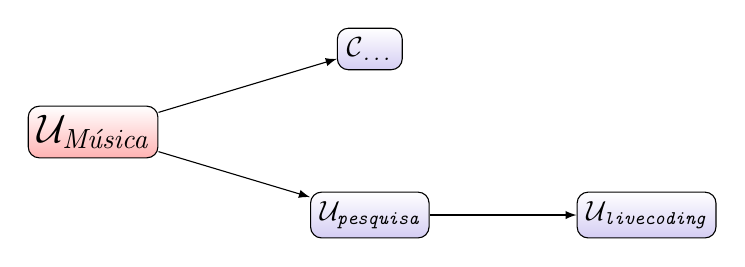
\begin{tikzpicture}
  [
    grow                    = right,
    sibling distance        = 6em,
    level distance          = 10em,
    edge from parent/.style = {draw, -latex},
    every node/.style       = {font=\footnotesize},
    sloped
  ]
  \node [root] {\csf{U}{Música}}
    child { node [env] {\csf{U}{pesquisa}}
      child { node [env] {\csf{U}{livecoding}}}
    }
    child { node [env] {\csf{C}{\ldots}}};
\end{tikzpicture}

No primeiro capítulo, incluímos um subjconjunto neste Espaço Conceitual da Pesquisa \ver{app:A}). 

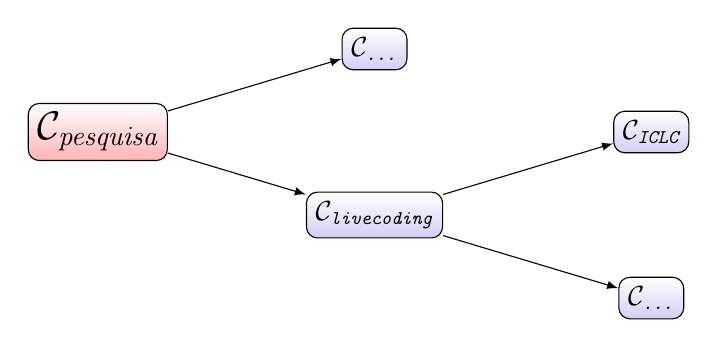
\begin{tikzpicture}
  [
    grow                    = right,
    sibling distance        = 6em,
    level distance          = 10em,
    edge from parent/.style = {draw, -latex},
    every node/.style       = {font=\footnotesize},
    sloped
  ]
  \node [root] {\csf{C}{pesquisa}}
    child { node [env] {\csf{C}{livecoding}}
      child { node [env] {\csf{C}{\ldots}}}
      child { node [env] {\csf{C}{ICLC}}}
    }
    child { node [env] {\csf{C}{\ldots}}}; 
\end{tikzpicture}

Podemos inclur elementos históricos, o período transitório entre 1970 e 2000 (\emph{circa}), onde emanciparam as práticas e as regras heurísticas.  

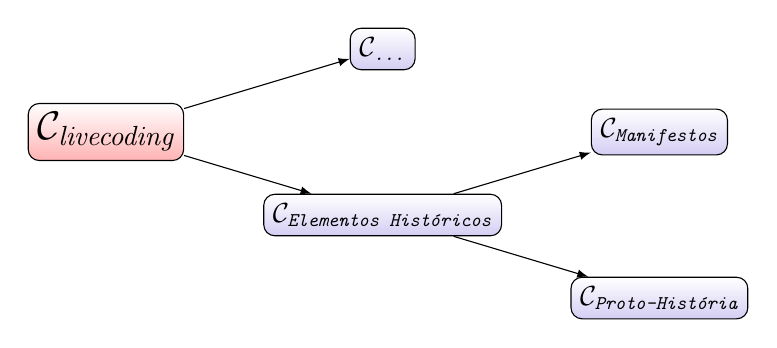
\begin{tikzpicture}
  [
    grow                    = right,
    sibling distance        = 6em,
    level distance          = 10em,
    edge from parent/.style = {draw, -latex},
    every node/.style       = {font=\footnotesize},
    sloped
  ]
  \node [root] {\csf{C}{livecoding}}
    child { node [env] {\csf{C}{Elementos Históricos}}
      child {node [env] {\csf{C}{Proto-História}}}
      child {node [env] {\csf{C}{Manifestos}}}
    }
    child { node [env] {\csf{C}{\ldots}}};
\end{tikzpicture}

Por último, \csf{C}{pesquisa} investiga o \emph{live coding} a partir de um caso específico:

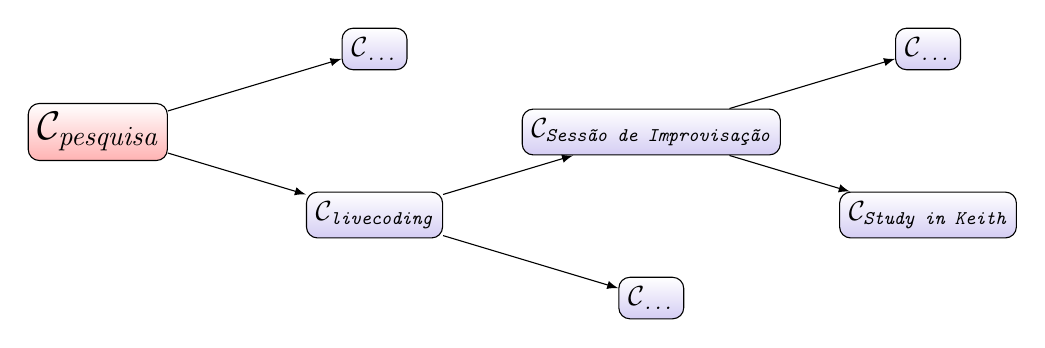
\begin{tikzpicture}
  [
    grow                    = right,
    sibling distance        = 6em,
    level distance          = 10em,
    edge from parent/.style = {draw, -latex},
    every node/.style       = {font=\footnotesize},
    sloped
  ]
  \node [root] {\csf{C}{pesquisa}}
    child { node [env] {\csf{C}{livecoding}}
      child { node [env] {\csf{C}{\ldots}}}
      child { node [env] {\csf{C}{Sessão de Improvisação}}
        child { node [env] {\csf{C}{Study in Keith}}}
        child { node [env] {\csf{C}{\ldots}}}
      }
    }
    child { node [env] {\csf{C}{\ldots}}}; 
\end{tikzpicture}
\end{example}

Por outro lado \csf{C}{Study in Keith} pode ser definido pelo modelo de improvisação de Pressing (\autoref{tab:modelo_improvisacao}, \pageref{tab:modelo_improvisacao}).

\begin{example}{Representação do modelo de improvisação para \emph{Study in Keith}.}
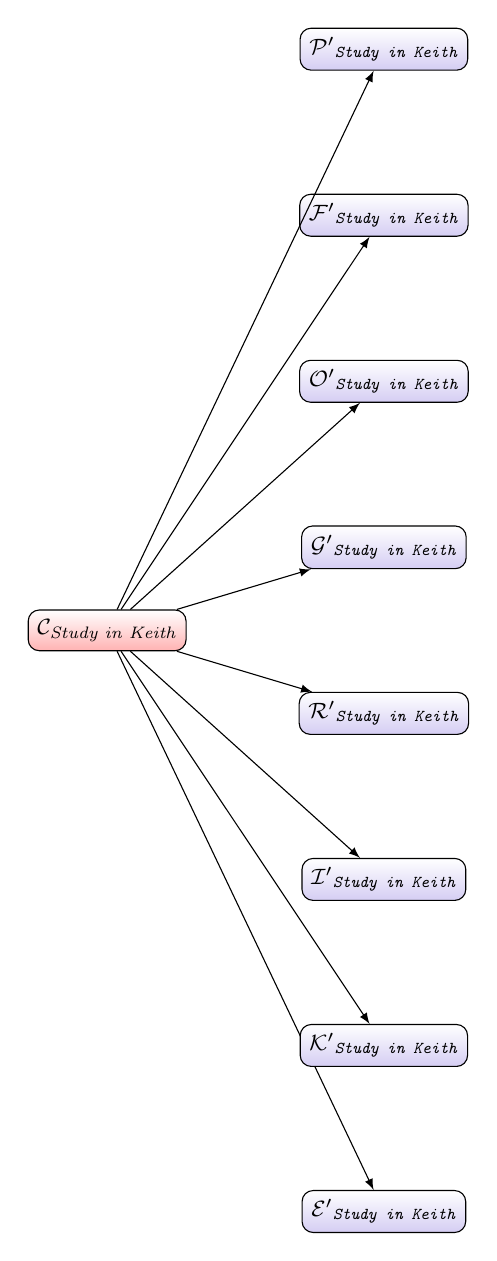
\begin{tikzpicture}
  [
    grow                    = right,
    sibling distance        = 6em,
    level distance          = 10em,
    edge from parent/.style = {draw, -latex},
    every node/.style       = {font=\footnotesize},
    sloped
  ]
  \node [root] {\footnotesize \csf{C}{Study in Keith}}
    child { node [env] {\footnotesize \csf{E'}{Study in Keith}}}
    child { node [env] {\footnotesize \csf{K'}{Study in Keith}}}
    child { node [env] {\footnotesize \csf{I'}{Study in Keith}}}
    child { node [env] {\footnotesize \csf{R'}{Study in Keith}}}
    child { node [env] {\footnotesize \csf{G'}{Study in Keith}}}
    child { node [env] {\footnotesize \csf{O'}{Study in Keith}}}
    child { node [env] {\footnotesize \csf{F'}{Study in Keith}}}
    child { node [env] {\footnotesize \csf{P'}{Study in Keith}}}; 
\end{tikzpicture}
\end{example}

\section{Formalização}\label{sec:formaliza}

O espaço conceitual do \emph{livecoding} é definido como uma função de interpretação das regras de validação (o que pode ser ou não considerado como próprio de uma categorização musical), de gosto (questões de estilo) e de localização transversal de conceitos (conceitos internos que permitem o cruzamento com outros conceitos). As regras de validação foram estudadas neste trabalho como as regras heurísticas do \emph{live coding}. Isto é, que conjunto de métodos são utilizados para caracterizar uma performance de \emph{live coding} como tal? Elementos históricos, e ideológicos (divulgados em manifestos), são levantados para responder esta pergunta. Por outro lado, este estudo abandonou a investigação das regras de gosto, tema que pode ser melhor explorado em trabalhos posteriores, a partir de \citeonline{janotti_jr._a_2003,sa_musica_2006,sa_se_2009}. A tarefa de localização transversal de conceitos é trabalhada no último capítulo. O espaço conceitual de \emph{Study in Keith} está contido no espaço conceitual do \emph{live coding} através da união entre os conceitos deste último, com os espaços conceituais dos concertos \emph{Sun Bears}, de Keith Jarret, misturados. No entanto o espaço conceitual não será investigado em sua totalidade, e sim apenas uma sonoridade.
\newpage
\chapter{Estudo de caso}\label{cap:estudos_de_caso}

Neste trabalho analisaamos a imagem mental de uma metáfora sonora, a partir de um espaço conceitual da Música. Dentro deste espaço conceitual, selecionamos um outro mais específico, que vem do \emph{jazz}. Nossa escolha busca ilustrar a readequação da figura do intérprete concertista para os propósitos do programador \ver{sec:obscurantismo}:

\begin{citacao}
\traducao{Para fundamentar a discussão em música, considere uma peça de \emph{jazz}, onde \emph{jazz} é um conceito e uma composição particular é uma instância de um conceito. O musicista, explorando os limites do \emph{jazz}, encontra então uma peça para além das regras usuais do \emph{jazz}. Através deste processo, os limites do gênero musica podem ser redefinidos em algum grau, ou se a peça está em um novo terreno particularmente fértil, um novo sub-gênero de \emph{jazz} emerge. Contudo uma peça de música que não quebra limites, de alguma forma pode ser considerada não-criativa. \cite[p.~117]{McLean2011}}{
To ground the discussion in music, consider a piece of jazz, where jazz is the concept and the particular composition is an instance of that concept. The musician, in exploring the boundaries of jazz, then finds a piece beyond the usual rules of jazz. Through this process, the boundaries of a music genre may be redefined to some degree, or if the piece is in particularly fertile new ground, a new sub-genre of jazz may emerge.  Indeed a piece of music which does not break boundaries in some way could be considered uncreative.}
\end{citacao}

O objetivo deste capítulo será detalhado na \autoref{sec:objetivo}. Seu contexto inicia com dois registros audiovisuais de \emph{A Study in Keith}, publicados por \citeonline{sorensen_youtube_2014} e \citeonline{sorensen_keith_2009}. São o mesmo registro, mas com duas descrições diversas de um mesmo espaço conceitual \csf{E}{ask}. Existe uma semelhança entre as explicações: um referente opcional \pressingthree{R}{ask}{0} são os Concertos \emph{Sun Bear} \ver{sec:sunbear}. \citeonline{sorensen_youtube_2014} indica outros referentes, \pressingthree{R}{ask}{1} como o ambiente de programação \emph{Impromptu} e \pressingthree{R}{ask}{2} a linguagem de programação \emph{Scheme} \ver{sec:impromptu}: 

\begin{citacao}
\traducao{\emph{A Study in Keith} é uma performance de programação ao vivo por Andrew Sorensen, inspirado nos concertos \emph{Sun Bear} de Keith Jarret. Toda a música que você ouve é gerada a partir do código do programa que é escrito e manipulado em \emph{tempo-real} durante a performance. O trabalho foi executado usando o ambiente de desenvolvimento $[$em linguagem$]$ Scheme $[$chamado$]$ Impromptu (\url{http://impŕomptu.moso.com.au}). Não é Keith, mas inspirado por Keith \cite{sorensen_youtube_2014}.
}
{
``A Study In Keith'' is a live programming performance by Andrew Sorensen inspired by Keith Jarrett's Sun Bear concerts. All of the music you hear is generated from the program code that is written and mani$[$p$]$ulated in real-time during the performance. The work was performed using the Impromptu Scheme software development environment (\url{http://impromptu.moso.com.au}). Not Keith, but inspired by Keith.
}
\end{citacao}

Uma breve análise de uma sonoridade cadencial de um dos concertos será investigada para encontrar outros possíveis referentes opcionais \ver{sec:sunbearanal}. As mensagens codificadas no ambiente \emph{Impromptu} são enviadas para um segundo \emph{software}, um instrumento virtual de estúdio (VSTi), que atua como um simulador de teste para a utilização em um instrumento acústico em uma vinheta nomeada \emph{Disklavier Sessions} \ver{sec:NI}. É indicado também um evento sonoro muito recorrente na improvisação de códigos. O silêncio é, com suas variações temporais, uma constante em outros trabalhos de Sorensen \ver{sec:silencio}:

\begin{citacao}
\traducao{\emph{A Study In Keith} é um trabalho para piano solo (NI's Akoustik Piano), inspirado nos concertos \emph{Sun Bear} de Keith Jarrett. \textbf{Note que não existe som durante os dois primeiros 2 minutos da performance, enquanto estruturas iniciais são construídas}. Não é bem Keith, mas inspirado por Keith \cite{sorensen_keith_2009}}{"A Study In Keith" is a work for solo piano (NI's Akoustik Piano) by Andrew Sorensen inspired by Keith Jarrett's Sun Bear concerts. Note that there is no sound for the first 2 minutes of the performance while initial structures are built. Not quite Keith, but inspired by Keith.}
\end{citacao}


\section{Objetivo}\label{sec:objetivo}

Como pontua \citeonline[p.~121]{McLean2011} \traducao{Nosso estudo de caso é de alguma forma simplista e não é intenção ilustrar uma grande arte ou um grande código. Contudo delineia um processo criativo de classes, como efetuado pelo presente autor.}{Our case study is somewhat simplistic, and is not intended to illustrate either great art or great code. However it does trace a creative process of sorts, as carried out by the present author.}

Este capítulo tratará sobre um grupo finito de blocos de eventos, $[$\pressingthree{E}{ask}{0}$,\ldots,$\pressingthree{E}{ask}{2}$]$, para investigar qual é um primeiro objetivo \pressingtwo{G}{0} \ver{sec:eventos}. Será apresentado também uma classe objetos \pressingtwo{O}{ask} (uma figura de notas) pertinente para entender como este início de improviso inclue uma característica \pressingtwo{F}{ask}{N} semelhante à \emph{Illiac Suite} de \citeonline{hiller_experimental_1959}, mas aplicado ao piano solo. 

\section{Referentes Opcionais}\label{sec:sunbear}

\subsection{Concertos Sun Bear}\label{sec:sunbearanal}

Os concertos \emph{Sun Bear} são originalmente dez LPs  de improvisações de Keith Jarret no Japão, produzidos pela \emph{ECM Records}\footnote{http://www.ecmrecords.com/} entre 1976 e 1978. É o terceiro dos concertos de improvisação que incluem o \emph{Solo Concerts: Bremen/Lausanne} (1973) e \emph{The Köln Concert} (1975).

Foram realizados e gravados como sessões de improvisação contínua, variando entre 31 a 43 minutos cada. Para cada dia, duas sessões de improvisação, em cidades diferentes. Kyoto, 5 de novembro\footnote{Disponível em \url{https://www.youtube.com/watch?v=T2TfIQNxhjc}.}; Osaka, 8 de novembro\disponivelem{https://www.youtube.com/watch?v=FC4iZ1wMoU8}; Nagoya, 12 de novembro\footnote{\url{https://www.youtube.com/watch?v=3a7ezm3D1jA}.}. Tokyo, 14 de novembro\disponivelem{https://www.youtube.com/watch?v=ZH8VIjjhPQ4}; Sapporo, 18 de Novembro\disponivelem{https://www.youtube.com/watch?v=BqYBT_HoG4M}.


Um documento crítico impresso é mencionado na \emph{internet} como um antigo documento contendo notas discográficas \cite{rollingstone1985}. Seu acesso foi restrito durante a pesquisa, e não foi possível incluir alguma citação. Da mesma forma, documentos análiticos sobre a peça não foram encontrados em alguma base de dados. Existem algumas notas discográficas compiladas por uma comunidade de fãs e críticos musicais estadounidenses. Duas notas sugerem uma descrição da forma musical aplicada por Keith Jarret: \traducao{O tema de \emph{Kyoto Parte 1} é repetido por Keith Jarret no fim de \emph{Kyoto Parte 2}. Então podemos considerar o todo deste concerto como uma grande Suíte.}{The theme of Kyoto Part 1 is repeated By Kj at the end of Kyoto Part 2. So we can consider the whole of this concert as one big Suite}\cite[p.~129]{jarret_discography_2014}. 

\traduzcitacao{Revisto por Richard S. Ginnel\footnote{Disponível em \url{http://www.mcana.org/formembersatlarge.html}.}: $[$--$]$ Este pacote gigantesco -- um conjunto de dez LPs agora comprimidos em uma caixa robusta de seis $[$embalagens de$]$ CDs -- foi ridicularizado uma vez como uma última viagem de ego, provavelmente por muitos que não tomaram um tempo para ouvir tudo. (\ldots) Ainda assim, o milagre é como esta caixa é consistentemente muito boa. \textbf{Na abertura de Kyoto, a meditação direcionada para o \emph{gospel}} está em plena atuação, ao nível de suas melhores performances solo em Bremen e Koln,\textbf{e os concertos Osaka e Nagoya possuem citações de primeira linha, geralmente do tipo \emph{folk}}, mesmo profundas, idéias líricas
}{
Review by Richard S. Ginell: $[$--$]$ This gargantuan package -- a ten-LP set now compressed into a chunky six-CD box -- once was derided as the ultimate ego trip, probably by many who didn't take the time to hear it all. You have to go back to Art Tatum's solo records for Norman Granz in the '50s to find another large single outpouring of solo jazz piano like this, all of it improvised on the wing before five Japanese audiences in Kyoto, Osaka, Nagoya, Tokyo, and Sapporo. Yet the miracle is how consistently good much of this giant box is.  In the opening Kyoto concert, Jarrett's gospel-driven muse is in full play, up to the level of his peak solo performances in Bremen and Koln, and the Osaka and Nagoya concerts have pockets of first-rate, often folk-like, even profound, lyrical ideas.
}
{p.~130}
{jarret_discography_2014}

O \emph{gospel} e o \emph{folk} são citados como gêneros musicais inclusivos nesta suíte. Porém esta Suíte não possui pausas entre as partes (o improviso é contínuo, mas seccionado por transições). Uma transcrição do motivo gerador deste \emph{gospel} no concerto de Kyoto buscou encontrar referentes opcionais adicionais para \pressingtwo{R}{ask} (isto é, informações de harmonia e ritmo), mesmo com a afirmação anterior que nenhuma relação pode ser encontrada \ver{fig:Jarret_intro}. 

\begin{figure}[!h]
  \centering
  %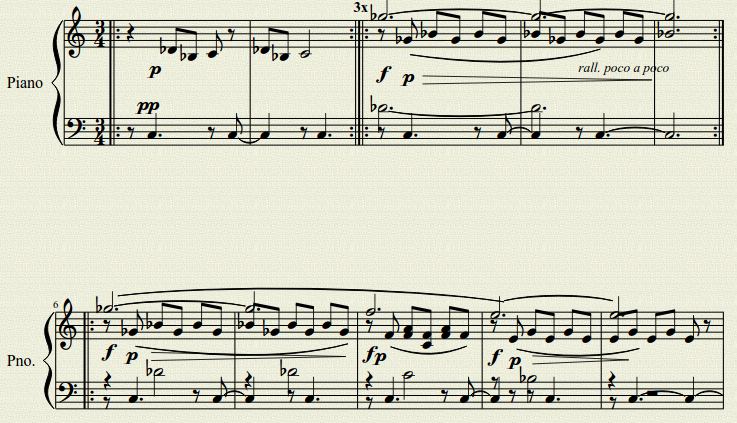
\includegraphics[scale=0.5]{imagens/Jarret_intro.png}
  {%
\parindent 0pt
\noindent
\ifx\preLilyPondExample \undefined
\else
  \expandafter\preLilyPondExample
\fi
\def\lilypondbook{}%
\input{b1/lily-fc418522-systems.tex}
\ifx\postLilyPondExample \undefined
\else
  \expandafter\postLilyPondExample
\fi
}
  \caption{Transcrição do motivo gerador do disco Kyoto, parte 1. \textbf{Fonte}: autor.}
  \label{fig:Jarret_intro}
\end{figure}

O bloco de sonoridades iniciais \pressingthree{E}{ask}{0} sugere alguma referência à forma Fantasia Cromática ou um Prelúdio, no sentido de um jogo livre que prepara o improvisador para a sonoridade do instrumento no ambiente tocado, com uma progressão bastante simples.  Uma sonoridade oscilante é colocada em movimento num âmbito de terça menor nos compassos 1 e 2 entre Si bemol, Dó e Ré Bemol, repetindo 3 vezes (\pressingthree{P}{KJ}{0}) dois objetos \pressingthree{O}{KJ}{0} e \pressingthree{O}{KJ}{1}: um ostinato na mão esquerda e uma bordadura na mão direita . Nos compassos 3 a 5 um terceiro objeto \pressingthree{O}{KJ}{2}, um acorde de Sol bemol Maior (transcrito assim para facilitar a leitura), dividido em uma quarta justa entre a mão esquerda e direita, com terças alternadas em colheias na mão direita. Este evento é então expandido nos compassos 6 a 10, gerando uma figura cromática proto-melódica, cujo acompanhamento harmônico segue uma progressão de substituição por trítono: Sol Bemol Maior, Fá Maior com sexta adicionada (ou Ré menor com sétima) e Dó Maior com sétima menor. Limitamo-nos a considerar esta progressão do ponto de vista do \emph{blues}, o que relacionaria com o \emph{gospel}. Por exemplo, a progressãopadrão  V$^7~\Rightarrow~$IV$^7~\Rightarrow~$I$^7$ pode ser transformada com substituições de dominantes e subudominantes. Uma operação comum é realizar uma substituição do grau V$^7~\Rightarrow~$bV$^7$. Porém Jarret suprime esta sétima, resultando em um bV. Já o quarto grau pode substituir  $IV^7~\Rightarrow~$IV$^6_5$. Neste sentido, com as devidas mudanças, este \emph{blues} é estruturado em uma sonoridade de tensão progressiva (tríade, tétrade de segundo grau invertido, e 'dominante'):  bV$~\Rightarrow~$IV$^6_5~\Rightarrow~$I$^7$ ou 1bV$~\Rightarrow~_3$II$^7~\Rightarrow~$I$^7$. 

\subsection{NI-Akoustik Piano}\label{sec:NI}

O NI, é uma abreviação para \emph{Native Instruments}, uma empresa de tecnologias para áudio \footnote{Disponível em \url{http://www.native-instruments.com/en/company/}.}. O \emph{Akoustic Piano} é uma extensão (\emph{plugin}) VST, que emula diferentes pianos acústicos. Entre os instrumentos utilizados, incluem o \emph{Bösendorfer 290 Imperial}, \emph{Steinway D}, e \emph{Bechstein D 280}\footnote{Disponível em \url{http://www.kvraudio.com/product/akoustik-piano-by-native-instruments}.}. Os instrumentos são gravados nota a nota por um complexo sistema de tomada de som. Na \autoref{fig:NI}, a gravação de um outro VSTi ilustra como é realizado o processo (no caso, por Uli Baronowsky)

\begin{figure}[!h]
  \centering
  %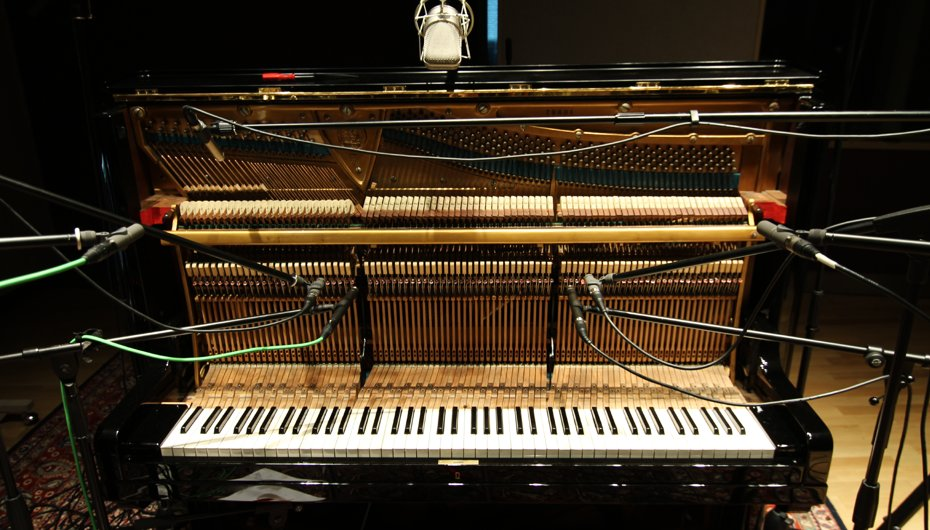
\includegraphics[scale=0.4]{imagens/piano.png}
  \caption{Sistema de tomada de som para produção de um VSTi. \textbf{Fonte}: \url{http://www.native-instruments.com/en/products/komplete/keys/definitive-piano-collection/}}
  \label{fig:NI}
\end{figure}

ou em um instrumento acústico modificado, como o \emph{Disklavier} da Yamaha \ver{fig:disklavier}. Este último caso não é citado por \citeonline{sorensen_youtube_2014} e \citeonline{sorensen_keith_2009}, masem \emph{Disklavier Sessions} \cite{sorensen_disklavier_2013} é semelhante à atividade descrita em \emph{A Study in Keith}:

\begin{figure}[h]
  \centering
  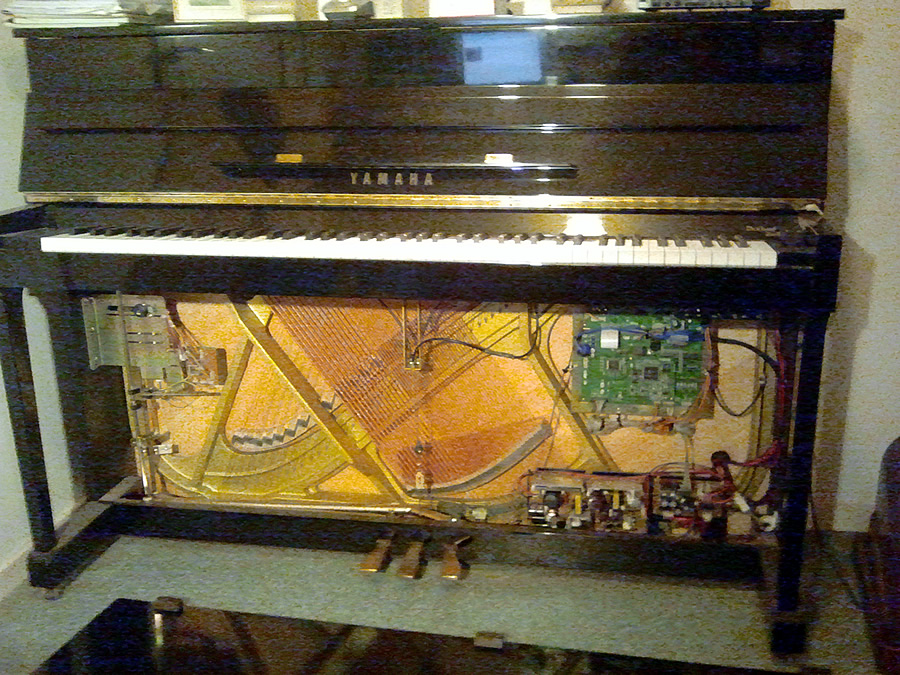
\includegraphics[scale=0.5]{imagens/disklavier.jpg}
  \caption{Piano Disklavier de armário, com a parte interna exposta para exibir a placa-mãe. \textbf{Fonte}: wikimedia.org}
  \label{fig:disklavier}
\end{figure}

\begin{citacao}
\traducao{Em \emph{Disklavier Sessions} os programas escritos em tempo-real por Ben e Andrew geram um fluxo de dados de notas que são enviados para ser executado em um piano disklavier mecanizado. Assim como as alturas das notas, toda a performance do piano deve ser codificada na informação gerada pelo programa e enviada para o piano disklavier.}{In the Disklavier Sessions the programs beign written in real-time by Ben and Andrew are generating a live stream of note data which is sent to a mechanized disklavier piano to be performed. As well the individual note pitches all of the piano performance must be encoded into the information being generated by the program and sent to disklavier piano}
\end{citacao}


\subsection{Ambiente e Linguagem: Impromptu}\label{sec:impromptu}

\begin{citacao}
\traducao{
Impromptu é uma linguagem e um ambiente de programação OSX\footnote{Sistema Operacional Mac OSX.} para compositores, artistas sonoros, VJ's e artistas gráficos  com um interesse em programação ao vivo ou interativa. Impromptu  é um ambiente de linguagem Scheme, um membro da família das linguages Lisp. Impromptu é usado por artistas-programadores em performances de \emph{livecoding} em torno do mundo.
}{
Impromptu is an OSX programming language and environment for composers, sound artists, VJ's and graphic artists with an interest in live or interactive programming. Impromptu is a Scheme language environment, a member of the Lisp family of languages. Impromptu is used by artist-programmers in livecoding performances around the globe.
}
\end{citacao}

Existe uma restrição quanto ao nicho de usuários do \emph{software}. É indicado que este grupo é restrito aos usuários de computadores Apple; no entanto uma investigação indica que o código-base é desenvolvido em um nível acima de outro, \emph{Extempore}.

\citeonline[p. 823] {sorensen_impromptu_2010} que o \emph{ambiente de programação ciberfísico} é análogo à \emph{partitura} tradicional; sua diferença está ligada à sua execução imediata. Nos termos de \citeonline{mathews_groove_1970}, uma \emph{engenharia humana}. Nos termos de \citeonline[p.~5]{fenerich_marulho_2014}, uma programação-partitura:

\begin{citacao}
\traducao{Considere a analogia da partitura musical tradicional. A partitura provê uma especificação estática da intenção -- um programa de domínio estático. Musicistas, representam o domínio do processo, executam ações requeridas para realizar ouo reificar a partitura. Finalmente, as ações no domínio do processo resultam em ondas sonoroas que são percebidas por uma audiência humana como música. Este estágio final é o nosso domínio real de trabalho. Agora considere um domínio de programação dinâmica no qual o compositor concebe e descreve uma partitura em \emph{tempo-real}. Nós geralmente chamamos este tipo de composição de improvisação. \textbf{Na improvisação o(a) musicista é envolvido em um circuito-fechado retroalimentado que envolve premeditação, movendo para ação casual e finalmente para reação, refinamento e reflexão.}}{
Consider the analogy of a traditional musical score. The score provides a static specification of intention – a static program domain. Musicians, representing the process domain, perform the actions required to realise or reify the score. Finally, the actions in the process domain result in sound waves which are perceived by a human audience as music. This final stage is our real-world task domain. Now consider a dynamic program domain in which a composer conceives of and describes a musical score in real-time. We commonly call this type of composition improvisation. In it, the improvising musician is involved in a feedback loop involving
forethought, moving to causal action and finally toreaction, refinement and reflection.}
\end{citacao}

\subsection{Extempore}

O \emph{Extempore} possui uma filosofia próxima àquela descrita por \citeonline{mathews_groove_1970}, isto é, de um sistema humano-máquina reflexivo. Um nome específico é dado para a atividade de escrita do código, ou \emph{programação ciberfísica}:

\begin{citacao}
\traducao{\emph{Extempore} é projetado para suportar um estilo de programação apelidado de $[$''$]$programação ciberfísica''.Programação ciberfísica suporta a noção de um programador humano operando como um agente ativo em uma rede de \emph{tempo-real} distribuída de sistemas ambientalmente conscientes} {Extempore is designed to support a style of programming dubbed 'cyberphysical' programming. Cyberphysical programming supports the notion of a human programmer operating as an active agent in a real-time distributed network of environmentally aware systems. \disponivelem{https://github.com/digego/extempore}. }
\end{citacao}

Entre suas características incluem\disponivelem{http://benswift.me/2012/08/07/extempore-philosophy/}:

- Processamento de Sinais Digitais (DSP) \footnote{Sobre DSP, \cfcite{smith_dsp_2012}.} em  tempo-real;

- Sequenciamento de áudio (baseado em notas) de alto-nível\footnote{Como o disparo de sons baseado em parâmetros como altura, intensidade e duração. Disponível em \url{http://benswift.me/2012/10/15/playing-an-instrument-part-i/}.};

- Processamento de gráficos;


A segunda característica será explorada neste capítulo como base técnica para o processo criativo em \emph{Study in Keith}

\subsection{Scheme}\label{sec:scheme}

Scheme (1970) é citado na \emph{internet} como uma definição de linguagem, ou dialeto, da linguagem Lisp (1958). Como uma linguagem imperativa orientada à expressões, utiliza \emph{representações simbólicas} de listas, para definir rotinas que podem definir outras rotinas. Esta característica habilitou programadores a realizarem uma atividade conhecida como \emph{meta-programação}.

\begin{example}{Notação Scheme}
Neste tipo de notação (\emph{prefix notation}, ou notação prefixada), são listados \emph{átomos}, que podem ser números, operadores, funções ou outras listas. Por exemplo. Uma divisão de dois números, pode ser escrita de maneira bastante simples:

\begin{minted}{cl}
;; uma operacao de divisao
(/ 1 2)

;; pode ser mais descritiva
(define divide (lambda (a b) (/ a b)))

;; execucao
(divide 1 2)
\end{minted}
\end{example}

Um exemplo musical é sugerido por \citeonline[p.~823-824]{sorensen_impromptu_2010} como fonte para um pseudo-código documentado. É possível notar uma ênfase em um discurso camerístico, na improvisação com instrumentos acústicos e sons eletrônicos, e uma base harmônica tonal comum:

\begin{example}{Exemplo imaginário}

NOTA: o processo será realizado de maneira semelhante àquele descrito por \citeonline{mathews_groove_1970} (\autoref{sec:groove}, p.~\pageref{sec:groove}), isto é, a partir de um circuito-fechado entre executante, máquina e projetores (visuais e acústicos).

\begin{citacao}
\traducao{
\small{Dois performers se apresentam no palco. Um violinista, em pé e parado, com seu arco preparado. Outro senta-se atrás do brilho da tela do \emph{laptop}. Uma projeção da tela do \emph{laptop} é projetada acima do palco, e mostra uma página em branco, com um simples cursor piscando. O musicista-programador começa a digitar \ldots}
}{
Two performers are present on stage. One, a violinist, stands paused, bow at the ready. Another sits behind the glow of a laptop screen. A projection of the laptop screen is cast above the stage showing a blank page with a single blinking cursor. The laptop musician begins to type ...
}
\end{citacao}

\begin{minted}{cl}
( play-sound ( now ) synth c3 soft minute)
\end{minted}

\begin{citacao}
\traducao{
\small{\ldots a expressao é avaliada, e lampeja no retroprojetor para exibir a ação do executante. Um som etéreo sintetizado entra imediatamente no espaço e o violinista começa a improvisar em simpatia com a novidade da textura. O músico-programador, ouve o material temático fornecido pelo violinista e começa a delinear um processo generativo Markoviano para acompanhar o violino:}
}
{
\ldots the expression is evaluated and blinks on the overhead projection to display the performer’s action. An ethereal synthetic sound immediately enters the space and the violinist begins to improvise in sympathy with the newly evolving synthetic texture. The laptop performer, listens to the thematic material provided by the violinist and begins to outline a generative Markov process to accompany the violin ...
}
\end{citacao}

\begin{minted}{cl}
( define chords
  ( lambda ( beat chord duration )
    ( for-each ( lambda ( pitch )
                   ( play synthj pitch soft duration ))
               chord )
    ( schedule (* metro * ( + beat duration )) chords
               (+ beat duration )
               ( random ( assoc chord (( Cmin7 Dmin7 )
                                       ( Dmin7 Cmin7 ))))
               duration )))

( chords (* metro * get-beat 4) Cmin7 4)
\end{minted}

\begin{citacao}
\traducao{\small{\ldots A função \emph{chords} é chamada no primeiro tempo de um novo xxxxxxx e uma simples progressão recursiva de acordes come a suportar a performance melódica do violino. A função \emph{chords} cria um laço temporal, gerando uma sequência interminável de acordes de quatro tempos. Depois de poucos momentos de reflexão, o musicista-programador começa a modificar a função \emph{chords} para suportar uma progressão de acordes mais variada, com uma razão aleatória $[$em função$]$ da recursão temporal\ldots}}
{\ldots the “chords” function is called on the first beat of a new common time bar and a simple recursive chord progression begins supporting the melodic performance of the violin. The chord function loops through time, creating an endless generative sequence of four beat chords. After a few moments of reflection the laptop performer begins to modify the “chords” function to support a more varied chord progression with a randomised rate of temporal recursion\ldots}
\end{citacao}

\begin{minted}{cl}
( define chords
  ( lambda ( beat chord duration )
    ( for-each ( lambda ( pitch )
                   ( play dls (+ 60 pitch) soft duration ))
               chord )
    ( schedule (* metro * ( + beat duration )) chords
               (+ beat duration )
               ( random ( assoc chord (( Cmin7 Dmin7 Bbmaj )
                                       ( Bbmaj Cmin7 )
                                       ( Dmin7 Cmin7 )))
               ( random (3 6))))))

( chords (* metro * get-beat 4) Cmin7 4)
\end{minted}
\end{example}

\section{Blocos de Eventos}\label{sec:eventos}

\subsection{Primeiro evento sonoro: a sensação de quietude}\label{sec:silencio}

Uma nota pertinente sobre esta improvisação é feita pelo próprio Sorensen: nos primeiros dois minutos do vídeo (aproximadamente 1$'$53$''$). existe um silêncio. Este silêncio é característico daquele momento em que os primeiros códigos são escritos.

Este comportamento, do tempo de codificação, ao tempo de ação musical, é similar em outros dois vídeos, de Sorensen: \sorensen{An evening of livecoding at 53 Rusden Street}{https://vimeo.com/2433303}, \sorensen{Just for Fun}{https://vimeo.com/2433971}, \sorensen{A Study in Part}{https://vimeo.com/2434054}, \sorensen{Stained}{https://vimeo.com/2502546}, \sorensen{Transmissions in Sound}{Transmissions in Sound}, \sorensen{Antiphony}{https://vimeo.com/2503188},  \sorensen{Strange Places}{https://vimeo.com/2503257}, \sorensen{Orchestral}{https://vimeo.com/2579694}, \sorensen{UMDT}{https://vimeo.com/2579880}, \sorensen{Day of Triffords}{https://vimeo.com/2735394}, \sorensen{Face to Face}{https://vimeo.com/5690854}, \sorensen{BM\&E}{https://vimeo.com/7339135}, \sorensen{A Christimas Carol}{https://vimeo.com/8364077} \sorensen{Dancing Phalanges}{https://vimeo.com/8732631}, \sorensen{Livecoding Audio DSP}{https://vimeo.com/15585520}, \sorensen{Jazz Ensenble Study}{https://vimeo.com/15679078}, \sorensen{Variations on a Christmas Theme}{https://vimeo.com/18008372}. Esta característica também foi observada em uma outra performance \ver{sec:concerto}.

\subsubsection*{Definição do instrumento e do tempo}

Seu início é um pequeno comentário que contêm o nome do executante e seu email para contato (primeiros sete segundos), bem como a escrita de um código que inicializa o NI-Akoustik (até 0$'$43$''$, ver \autoref{fig:SIK_piano}). 

\begin{example}{Definição de instrumento}
  \centering 
Primeiros eventos musicais gerados a partir das primeiras estruturas válidas de código. \textbf{Fonte}: \cite{sorensen_youtube_2014}.
  \begin{minted}[fontsize=\footnotesize]{cl}
    ;;;;;;;;;;;;;;;;;;;;;;;;;;;;;;;;;;;;;;;;;;;;;;;;;
    ;; Andrew Sorensen andrew@moso.com.au
    (define piano (au:make-node "aumu" "NaDd" "-NI-"))
    (au:connect-node piano 0 *au:output-node* 0)
    (au:update-graph)

    (au:load-preset piano "/tmp/convert_grand.aupreset")
  \end{minted}
  \label{fig:SIK_piano}
\end{example}

\newcommand{\tempo}[2]{#1$'$#2$''$}

Em \tempo{0}{52} Sorensen define um tempo base (ver \autoref{fig:SIK_metro}). Em seguida, Sorensen apaga o código para então iniciar definições de notas (\tempo{0}{54}).

\begin{example}{Definição de tempo}
  \centering
Definição do tempo base. \textbf{Fonte}: \cite{sorensen_youtube_2014}.
  \begin{minted}[fontsize=\footnotesize]{cl}
    (define *metro* (make-metro 110))
  \end{minted}
  \label{fig:SIK_metro}
\end{example}

\subsubsection*{Alternativas à definição de um instrumento}

Basicamente, o que foi desenvolvido no primeiro exemplo da seção anterior \ver{fig:SIK_piano}, recorre à uma definição customizada de amostras sonoras de um \emph{plugin} VST. Ben Swifth, co-desenvolvedor do Extempore, sugere outras maneiras de definir um instrumentos. Duas diferentes maneiras incluem a a utilização de amostras sonoras prédefinidas e organizadas\disponivelem{http://benswift.me/2012/10/17/loading-and-using-a-sampler/}, ou o processamento de sinal digital (DSP), através de definições de cada parâmetro do instrumento criado\disponivelem{http://benswift.me/2012/09/28/making-an-instrument/}. 

\subsubsection*{Definição de uma sequência de blocos}

Até \tempo{1}{07}, uma sequência de blocos \pressingtwo{K}{ASK} é definida, sem definir quais são os \pressingtwo{E}{ASK} que constituem. Isto é, definições de funções podem são alocadas hierarquicamente, sem definir o que está na estrutura mais interna.No caso o laço iterativo (\mint{cl}|pc:cb-for-each-p|) chama por acordes (\mint{cl}|chords|), cujos parâmetros são três: i) \mint{cl}|piano (pc:make-chord 50 70 2 (pc:diatonic 0 '- degree))|; ii). (ainda não sabemos quais são, o que caracteriza uma memória particular já interiorizada por Sorensen; isto é, ele ensaiou essa improvisação). (que  \ver{fig:SIK_acorde}.  Para cada acorde, é chamada uma a função que ainda não existe, \emph{chords}. Esta função é acompanhada de uma lista de 4 parâmetro (50, 70, 2). O último parâmetro é uma função de \emph{callback}, ou uma função que será executada

\begin{example}{Definição da sequência de blocos}
  \centering
Criação da rotina que irá executar acordes. \textbf{Fonte}: \cite{sorensen_youtube_2014}.
  \begin{minted}[fontsize=\footnotesize]{cl}
    (pc:cb-for-each-p chords piano
                      (pc:make-chord 50 70 2 (pc:diatonic 0 '- degree))
                      dur)
  \end{minted}
  \label{fig:SIK_acorde}
\end{example}

\subsubsection*{Definição de blocos}

Em 1$'$53$''$ a função \emph{chords} é definida de maneira válida, e os primeiros eventos sonoros são criados (ver \autoref{fig:SIK_acorde2}):

\begin{example}{Algoritmo que define os acordes}
  \centering
Definição da função \emph{chord}. \textbf{Fonte}: \cite{sorensen_youtube_2014}.
  \begin{minted}[fontsize=\footnotesize]{cl}
    (define chords
       (lambda (time degree dur)
          (if (member degree '(i)) (set! dur 3.0))
          (for-each (lambda (p)
                       (play-note (*metro* time) piano p
                                  (+ 50 (* 20 (cos (* pi time))))
                                  (*metro* 'dur dur)))
                    (pc:make-chord 50 70 2 (pc:diatonic 0 (quote -) degree)))
          (callback (*metro*) (+ time (* .5 dur))) chords (+ time dur)
                    (random (assoc degree '((i vii)
                                            (vii i))))
                    dur)))
    
     (chords (*metro* 'get-beat 4.0) 'i 3.0)
  \end{minted}
  \label{fig:SIK_acorde2}
\end{example}

O restante da improvisação será conduzida a partir da modificação desta função, que a cada tempo, executa um conjunto de notas (inicialmente blocos musicais, que desenvolve para contrapontos floridos, ostinatos e gestos  arpejo/escala), conforme é indicado pelo programador.


\subsection{Segundo Evento Sonoro}\label{sec:segundoevento}

Uma escuta investigativa desta performance considerou o resultado sonoro gerador como replicante de uma escrita contrapontística modal, não-estrita, inicialmente à duas vozes em primeira espécie, que lembra um canto religioso.

Sorensen define um tempo regular de 110 BPM durante o momento de silêncio Os primeiros eventos sonoros que ocorrem após o momento de silêncio foram transcritos considerando a percepção dos tempos fortes e fracos. Isto é, enquanto Sorensen define um tempo regular de 110 BPM, o processo de transcrição
de maneira aproximada em um tempo regular de aproximadamente 40 BPM. A partir disso, cada compasso desta transcrição são dois compassos do vídeo. Segundo o próprio vídeo, o tempo é definido por 110 BPM e cada nota inicial é de quatro tempos, mas que irá sofrer alterações. 

A \autoref{fig:SIK_acorde2} indica que um jogo entre primeiro grau menor, e sétimo grau diminuto será conduzido  (ver \autoref{fig:SIKinicio}).

\begin{figure}[!h]
  \centering
  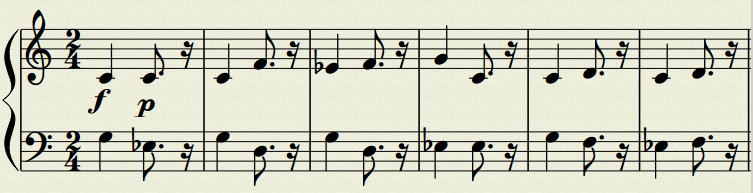
\includegraphics[scale=0.5]{imagens/SIK_motivo.png}
  \caption{Primeiros eventos musicais gerados a partir das primeiras estruturas válidas de código. \textbf{Fonte}: autor.}
  \label{fig:SIKinicio}
\end{figure}

Uma pequena transcrição de uma primeira seção da improvisação é apresentada na \autoref{app:studyinkeith}: uma primeira seção da peça, que vai do 1$'$53$''$ até 4$'$55$''$, pode ser descrita como: um contraponto, inicialmente à duas vozes em primeira espécie (dó eólio), que sofre perturbações sistêmicas. Tais perturbações parecem ser derivadas das intervenções de Sorensen no código do programa.

Tais perturbações criam variações na acentuação, bem como adicionam novas figuras de ritmo, de maneira bastante gradual (ver \autoref{fig:perturba}).

\begin{figure}[!h]
  \centering
  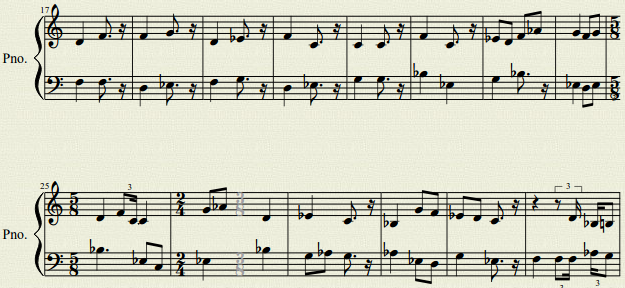
\includegraphics[scale=0.5]{imagens/SIK_perturba.png}
  \caption{Primeiros perturbações sistêmicas. \textbf{Fonte}: autor.}
  \label{fig:SIKinicio}
\end{figure}

No ponto culminante da peça podemos escutar um contraponto florido, adicionado de um ostinato com uma única nota, e algumas intervenções de gestos, arpejos ou escalas em alta velocidade.\todo{\tiny Este conceito nos pareceu bastante similar àquele apresentado por \citeonline{hiller_experimental_1959}. HillerDurante um breve período, algumas regras de contraponto não mantidas}

\subsection{Terceiro Evento Sonoro}\label{sec:terceiro evento}
\newpage

% ---
% Conclusão
% ---
\chapter*[Conclusão]{Conclusão}\addcontentsline{toc}{chapter}{Conclusão}\label{conclusao}

%\begin{citacao}
%``O marquês de X tem, como se sabe, um belo gabinete de física, mas a Eletricidade é sua paixão e, se o paganismo ainda vigorasse, ele decerto ergueria altares elétricos. Ele sabia quais são minhas preferências e não ignorava que também sou fã da \emph{Eletromania}. Convidou-me, portanto, para um jantar onde estariam presentes, segundo ele, os medalhões da ordem dos eletrizantes e das eletrizadas''. Conviria conhecer essa eletricidade falada que, sem dúvida, revelaria muito mais sobre a psicologia da época do que sobre sua ciência\footnote{Bachelard, G. \textit{A formação do espírito científico}. p.~41. Ed. Contraponto. Trad. Estela dos Santos de Abreu 1938 -- 1996}.
%\end{citacao}

Estimulada por artistas-programadores(as), a interiorização de um processo criativo (bricolagem) pode ter conduzido à formação de programas de pesquisas interdisciplinares, entre computação, cognição e práticas musicais tonais. Isto é, teorias das Artes Músicais, Audiovisuais, Corporais, Têxteis, Filosofia, e se a criatividade permitir, da Engenharia Crítica, são apropriadas para elaboração de conceitos. Uma classe particular de artistas-programadores(as) \cite[p.~16]{McLean2011}, o(a) improvisador(a) de códigos (\emph{live coder}), admite conhecimentos da engenharia de computação, revisada sob o prisma de uma ou mais teorias como extensão para improvisações ou ou análise de registros. O improvisador de códigos, em geral, pratica o \emph{live coding} segundo uma cultura de publicações, sejam elas divulgadas na \emph{internet}\disponivelem{http://www.toplap.org}, deselvolvida a partir de \cite{ward_live_2004}, em revistas de programas de investigação científica, como  \emph{Computer Music Journal}, \emph{Leonardo}, em listas de email de \emph{softwares}. Por fim, é estimulado codificar programas, não como um produto de venda, mas para fins pedagógicos, musicais, audiovisuais, têxteis e filosóficos. 

%Por exemplo, um duo de improvisadores-programadores (\emph{live coders}), cada um com sua programação-partitura\footnote{\cfcite[p.~5]{fenerich_marulho_2014}.}, executam uma performance artítica \ver{fig:toalete}.

%\begin{figure}[h]
%    \centering
%    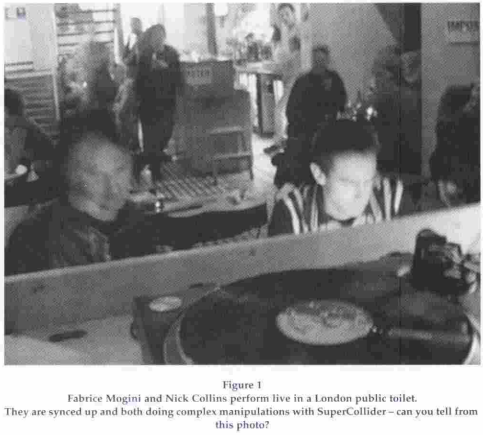
\includegraphics[scale=0.71]{imagens/toalete.png}
%    \caption{ ``Fabrice Mogini e Nick Collins tocando ao vivo em um banheiro público de Londres. Eles estão sincronizados e ambos fazendo manipulações complexas com o \emph{SuperCollider}.''. \textbf{Fonte}: \citeonline{collins_generative_2003}.}
%    \label{fig:toalete}
%  \end{figure}


%\begin{citacao}
%\emph{Programação imediata} (ou: programação de conversa, programação no fluxo, programação interativa) é um paradigma que inclue a atividade de programação ela mesma como uma operação do programa. Isto significa um programa que não é tomado como ferramenta que cria primeiro, e depois é produtivo, mas um processo de construção dinâmica de descrição e conversação - escrever o código e então se tornar parte da prática musical ou experimental. \cite[Verbete JITLib]{supercollider.org_supercollider_2014}\footnote{Tradução de \emph{Just in time programming (or: conversational programming, live coding , on-the fly-programming, interactive programming) is a paradigm that includes the programming activity itself in the program's operation. This means a program is not taken as a tool that is made first, then to be productive, but a dynamic construction process of description and conversation - writing code thus becoming a closer part of musical or experimental practice.}}
%\end{citacao}

\citeonline{ward_live_2004} definem a improvisação de códigos como \traducao{atividade da escrita integral (ou partes) de um programa enquanto ele é executado}{Live coding is the activity of writing (parts of ) a program while it runs}. \citeonline{blackwell_programming_2005} enfatizam a definição do ponto de vista da linguagem de programação como instrumento musical. \citeonline{mclean_hacking_2006} relata o \emph{live coding} como ferramenta para um \emph{Disk Jockey codificado}.  \citeonline{sorensen_keith_2009} pontuam a improvisação de códigos como \traducao{uma prática de performance para o qual linguagens de computador definem o meio primário de expressão artística.}{Live coding is a performance pratice for which computer languages define  the primary means of expression.}. Para \citeonline{sorensen_impromptu_2010}, \emph{live coding} (ou \emph{livecoding}) envolve a premissa de uma programação-partitura audiovisual reativa: 

\traduzcitacao{
Livecoding é uma prática de arte computacional que envolve criação em tempo-real de programas de audiovisual generativo para performances multimídias interativas. Comumente as ações dos programadores são expostas para uma audiência por projeção do ambiente de edição. Performances de livecoding geralmente envolvem mais de um participante, e são geralmente iniciadas a partir de uma folha conceitual em branco   
}{Livecoding [10, 50] is a computational arts practice that involves the real-time creation of generative audiovisual software for interactive multimedia performance. Commonly the programmers’ actions are exposed to the audience by projection of the editing environment. Livecoding performances often involve more than one participant, and are often commenced from a conceptual blank slate}
{p.~823}
{sorensen_impromptu_2010}

\citeonline{magnusson_algorithms_2011,collins_origins_2014} sintetizam o \emph{live coding} como improvisação audiovisual. \citeonline{sorensen_programming_2014} define como \traducao{programar sistemas de tempo-real em tempo real}{programming real-time systems in real-time}. Em um discussão entitulada ``\emph{Wtf is livecoding}''\disponivelem{http://lurk.org/groups/livecode/messages/topic/ofAxZpxsKFpDRLnoA48Bh} diz que o \traducao{\emph{Live coding} celebra a efemeridade da própria definição}{Live coding celebrates the ephemerality of definition itself} \ver{fig:live_coding_def}.

Embora semelhantes, as definições mudam de detalhes de acordo com o contexto. Por exemplo, \citeonline{ward_live_2004} enfatizam que o código pode ser (re)composto de partes menores. \citeonline{mclean_hacking_2006} pontua o ambiente de codificação onde o código é (re)programado, e que tipo de música é feita. \citeonline{sorensen_programming_2014} destaca que modificar alguma coisa (bricolagem) é próprio da técnica, de forma que é possível extender essa bricolagem para ideologias, enfraquecendo a própria definição de \emph{live coding}. Nick \citeonline{collins_origins_2014} situa essa questão da seguinte formafundamentos objeto:

  \begin{figure}[h]
    \centering
    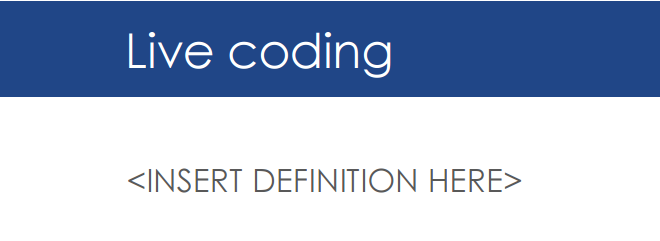
\includegraphics[scale=0.7]{imagens/live_coding_def.png}
    \caption{Definição de \emph{live coding}: ``Insira a definição aqui''. \textbf{Fonte}: \citeonline{collins_origins_2014}.}
    \label{fig:live_coding_def}
  \end{figure}


Se por um lado a definição agrega definições, o que dificulta a tarefa inicial de descrever os fundamentos do objeto de pesquisa, por outro ilustra a improvisação de códigos como um \emph{Universo de conceitos}. Neste trabalho consideramos que definições ou performances de improvisação de códigos estão contidas em diferentes \emph{Espaços Conceituais} \cite{wiggins_framework_2006,mclean_music_2006}. Artistas-programadores (\emph{live coders}) transitam entre os Espaços Conceituais para criação de Sistemas Criativos (códigos, programas). Estes Sistemas Criativos são representados em diferentes Linguagens de Programação. Regras práticas conduzem o processo de escrita e exposição desta linguagem; mas não restringem o resultado (no caso da pesquisa, musical). Mas algumas categorizações musicais se destacam.  Neste sentido, selecionamos um exemplo simbólico, \emph{A Study in Keith} de Andrew \citeonline{sorensen_keith_2009}\footnote{Disponível em \url{https://vimeo.com/2433947}.}. Representa um caso particular que foge dos exemplos citados anteriormente, mas envolve a manutenção de uma tradição musical tonal através de um interessante esforço de \emph{replicação do estilo}. 

No \autoref{cap:introducao} selecionamos alguns exemplos afim de ilustrar nossa percepção (conhecimento-psicológico) do imaginário daquilo que \citeonline{McLean2011} chama de artistas-programadores. No \autoref{cap:protohistoria} buscamos levantar um conjunto de conhecimentos históricos. No \autoref{cap:metodologia}, discutimos um modelo de formalização conceitos, observados pelo prisma de Alex \citeonline{mclean_music_2006}, contraposto por \citeonline{thornton_quantitative_2007}, e rediscutido por \citeonline{McLean2011}, \citeonline{Forth2011}. No \autoref{cap:estudos_de_caso}, organizamos conceitos de um algoritmo inicial de uma improvisação de códigos, \emph{A Study in Keith} de 2009, segundo este um Quadro Conceitual de Sistemas Criativos . 

Por último, esta conclusão, é mais uma reflexão sobre o processo de pesquisa. Do ponto de vista apresentado na Introdução, interpretamos algumas práticas da improvisação de códigos como parte de uma cultura cognitivo-capitalista; isto é, no qual o capital simbólico é representado não mais por cifras impressas em papel, ou memorizadas em um sistema bancário através de créditos. O capital em questão são conhecimentos que, de tão especificados, podem criar a estranha imagem de escravos que negociam com seus senhores em qual jaula serão encarcerados. Neste sentido, apresentamos no \autoref{app:A}, o processo de organização qualitativa de conceitos sobre o \emph{live coding}, em um congresso realizado pelo \citeonline{ICLC2015}, de forma que este material de pesquisa estimulou o interesse pelo tema discutido.

% ---
% Bibliografia
% ---
\bibliography{main}

% ----------------------------------------------------------
% Glossário
% ----------------------------------------------------------
%
% Consulte o manual da classe abntex2 para orientações sobre o glossário.
%
%\glossary

% ----------------------------------------------------------
% Apêndices
% ----------------------------------------------------------

% Imprime uma página indicando o início dos apêndices
%\partapendices

% ---
% Inicia os apêndices
% ---
\begin{apendicesenv}
\chapter{Código fonte de um Universo Conceitual como nuvem de palavras sobre o improviso de códigos}\label{app:A}

O tema da improvisação de códigos, como um universo de conceitos, surgiu de uma experiência com um código em linguagem \emph{python}\disponivelem{https://www.python.org/}, útil para gerar um mapa de termos, como ilustrado na figura \autoref{fig:nuvemlivecoding}

\begin{figure}[!h]
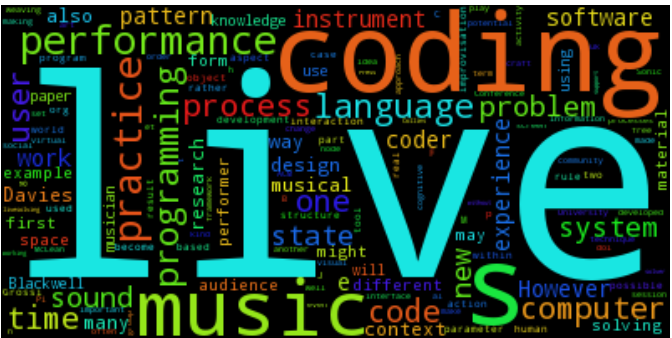
\includegraphics[scale=0.8]{imagens/nuvem.png}
\caption{Nuvem de palavras do \citeonline{ICLC2015},  1$^o$ Congresso Internacional de Live Coding. \textbf{Fonte}: autor.}
\label{fig:nuvemlivecoding}
\end{figure}

A imagem acima foi gerada com um código nomeado como \emph{cloupdf.py}, e considera seguinte situação, subdividida em três passos: 

1) Converter um arquivo de texto, ou um conjunto de textos cientítificos, em formato \emph{.pdf} para formato \emph{.txt}; 

2) Feita a conversão, plotar uma imagem com as palavras mais relevantes, do ponto de vista quantitativo; 

3) Desta plotagem, organizar as palavras qualitativamente, de acordo com suas funções gramaticais no texto, em classes quantitativas (ver \autoref{tab:gen1}, p.~\pageref{tab:gen1}; \autoref{tab:gen2}, p.~\pageref{tab:gen2}; \autoref{tab:gen3}, p.~\pageref{tab:gen3}; \autoref{tab:gen4}, p.~\pageref{tab:gen4}; \autoref{tab:gen5}, p.~\pageref{tab:gen5}).

\begin{example}{Código-fonte do \emph{cloud.py}}
\begin{minted}[fontsize=\scriptsize]{python}
#!/usr/bin/python

# Algumas bibliotecas principais
from wordcloud import WordCloud     # Nuvem de palavras
import nltk                         # Processamento de linguagem natural
import matplotlib.pyplot as plt     # Desenha foto
from subprocess import Popen, PIPE  # Acessa um o conversor de pdf
from optparse import OptionParser   # Cria um programa

# Bibliotecas basicas
from os import path
import math

# PROGRAMA PRINCIPAL
def linha_de_comando(nome, versao, descricao): 
    parser = OptionParser(usage='usage: %prog [OPTIONS, [ARGS]]', 
                          version='%s %s' % (nome, versao), 
                          description=descricao)
    # Cria opcoes
    parser.add_option("-e","--entrada",
                      action=None,
                      help="arquivo pdf de entrada",
                      dest="input",default=False)
    parser.add_option("-q","--qualidades",
                      action=None,
                      help="classificacao por qualidades (0..n-1)",
                      dest="qualidades",
                      default=False)
    parser.add_option("-f","--foto",
                      action="store_true", 
                      help="arquivo de saida da foto",
                      dest="fotinha",
                      default=False),
    parser.add_option("-p","--paginas",
                      action=None,
                      help="paginas processadas",
                      dest="paginas",
                      default=False)
    parser.add_option("-c","--codec",
                      action=None,
                      help="tipo de codificacao do texto",
                      dest="codec",
                      default=False)
    parser.add_option("-t","--table",
                      action=None,
                      help="converte a nuvem para uma tabela: \n\t-tex (suportado)\n\t-mardown (planejado)",
                      dest="table",
                      default=False)

    # Life cycle
    (options, args) = parser.parse_args()
    pages = []
    if options.paginas:
        split =  options.paginas.split("..") 
        a = [ str(s) for s in range(int(split[0]), int(split[1])) ]
        pages = ",".join(a)
    else:
        pages = [1,2]
    text = convert_pdf_to_txt(options.input,pages,options.codec)
    
    # Nuvem
    print "\n\nA gerar nuvem ..."
    nuvem = WordCloud().generate(text)
    print "=> Feito"
    if options.fotinha:
        gera_figura(nuvem)
    
    #if options.table:
    # Taggins
    print "\n\nA classificar e organizar palavras em uma tabela"
    tagging = nltk.pos_tag(nltk.word_tokenize(text))
    qualidades = gera_grupos_qualitativos(nuvem, tagging, int(options.qualidades) or 10)
    nome = options.input.split(".tex")[0]
    f = open("%s.tex" % options.table, "w+")

    #    if options.table is "tex":
    tabela_tex = table(qualidades, options.qualidades, options.table, "tab:gen").decode(options.codec)
    f.write(tabela_tex)
    f.close()
    print "=> Feito: %s.tex" % options.table
    
#http://davidmburke.com/2014/02/04/python-convert-documents-doc-docx-odt-pdf-to-plain-text-without-libreoffice/
#http://stackoverflow.com/questions/5725278/python-help-using-pdfminer-as-a-library
def convert_pdf_to_txt(p, pages, codec):
    name = p.split(".pdf")[0].split("/")[-1]
    _path = path.abspath("%s.txt") % name
    print "A converter %s para %s  ... \n\n" % (p,_path)
    command = "=> pdf2txt.py -o %s -p %s -c %s %s" % (_path, pages, codec, p)
    print command
    #https://stackoverflow.com/questions/24340877/why-does-this-bash-call-from-python-not-work
    result = Popen(command, stdout=PIPE, shell=isinstance(command, str))
    #print result.communicate()
    print "=> ... checking ascii characters"
    f = open(_path)
    s = ""
    for i, line in enumerate(f.readlines()):
        l = line.decode(codec)
        s += l

    print "=> Feito"
    return s
    
# gera figura a partir da nuvem
def gera_figura(nuvem):
    print "A gerar uma nuvem de palavras..."
    plt.figure()
    plt.imshow(nuvem)
    plt.axis("off")
    print "=> Pronto"
    plt.show()
    
###
# CC: conjunction, coordinating
# CD: numeral, cardinal
# DT: determiner
# EX: existential there
# FW: foreign word
# IN: preposition or conjunction, subordinating
# JJ: adjective or numeral, ordinal
# JJR: adjective, comparative
# JJS: adjective, superlative
# LS: list item marker
# MD: modal auxiliary
# NN: noun, common, singular or mass
# NNP: noun, proper, singular
# NNPS: noun, proper, plural
# NNS: noun, common, plural
# PDT: pre-determiner
# POS: genitive marker
# PRP: pronoun, personal
# PRP$: pronoun, possessive
# RB: adverb
# RBR: adverb, comparative
# RBS: adverb, superlative
# RP: particle
# SYM: symbol
# UH: interjection
# VB: verb, base form
# VBD: verb, past tense
# VBG: verb, present participle or gerund
# VBN: verb, past participle
# VBP: verb, present tense, not 3rd person singular
# VBZ: verb, present tense, 3rd person singular
# WDT: WH-determiner
# WP: WH-pronoun
# WP$: WH-pronoun, possessive
# WRB: Wh-adverb
###
def criaGrupos(nuvem, tagging, n, groups={}):
    # primeiro crie uma tabela das funcoes:
    for tag in tagging:
        if not str(tag[1]) in groups:
            groups.__setitem__(tag[1], {})
        
        for t in nuvem.words_:
            freq = t[1]
            index = int(math.floor(freq*n))
            if not str(index) in groups.__getitem__(tag[1]):
                groups.__getitem__(tag[1]).__setitem__(str(index), [])

            word = t[0].title()
            t = tag[0].title()
            if word == t:
                if not word in groups.__getitem__(tag[1]).__getitem__(str(index)):
                    groups.__getitem__(tag[1]).__getitem__(str(index)).append(word)

        for i in range(n):
            if not str(i) in groups.__getitem__(tag[1]):
                groups.__getitem__(tag[1]).__setitem__(str(i), [])
                
    return groups

def gera_grupos_qualitativos(nuvem, tagging, n):
    return criaGrupos(nuvem, tagging, n)

def table(groups, size, caption, label):
    print "=> creating table for %s" % caption
    print groups
    string =  """\\begin{table}
\\centering
\\caption{%s}
\\label{%s}
\\small
\\begin{tabular}{""" % (caption, label)
    string = string + "%s" % "".join([" | p{1cm}" for i in range(int(size)+2)])
    string = string + """ |}
\\hline
\\hline
"""
    # Cabecalho geral
    string = string+ "\\tiny \\textbf{Qualidade/Funcao}\n"
    for i in range(int(size)):
        if i is not int(size)-1:
            string = string + " & \\textbf{%s}\n" % i
        else:
            string = string + " & \\textbf{%s} \\\\ \n" % i
    string = string + "\\hline\n\\hline\n"

    # conteudo again:
    for k, v in groups.iteritems():
        string = string + "\\tiny \\textbf{%s}\n" % k 
        a = range(int(size)+1)
        for i in a:
            string = string + " & \\tiny"
            if len(v[str(i)]) is 0:
                string = string + " -- "
            else:
                string = string + " %s " % ", ".join(v[str(i)])
    
            if i is len(a) :
                string = string + " \\\\ \n"
        string = string + "\\hline\n"
            
    string = string +  """
\\hline
\\end{tabular}
\\end{table}
"""
    print string
    return string
    
linha_de_comando("claudio", "0.0.1", "Script python para gerar nuvem de arquivos pdf")


\end{minted}
\end{example} 

\section{Utilização}

Em um terminal Linux (3.16.0-49-generic, Ubuntu 14.04.1, i686), executamos o código como um comando  com opções de: 1) arquivo de entrada (\verb|--entrada| ou \verb|-e|), número de páginas rastreadas (\verb|--paginas| ou \verb|-p|), classes (\verb|--qualidades| ou \verb|-q|), codificação do pdf (\verb|--codec| ou \verb|-c|), criação de uma nuvem de palavras (\verb|--foto| ou \verb|-f|) e organização de uma tabela (\verb|--table| ou \verb|-t|). 

Este código utilizou três bibliotecas auxiliares \emph{pdf2text.py}\disponivelem{https://pypi.python.org/pypi/pdf2text}, \emph{Wordcloud}\disponivelem{https://github.com/amueller/word_cloud} e \emph{NLTK}\disponivelem{http://nltk.org/}. 

A primeira biblioteca permite extrair do pdf caracteres válidos para análise. A segunda biblioteca realiza o levantamento de dados. E a terceira biblioteca auxilia na organização das funções gramaticais. Essas operações serão exemplificadas na próxima seção.

\section{Experiências}

Durante uma primeira experiência, abrimos um arquivo pdf, mais especificamente os anais de um congresso internacional \cite{ICLC2015}, e organizamos algumas páginas pertinentes, neste caso, todas a páginas com o corpo de texto (p. 4 -- 230),  supostamente codificado em um padrão ISO8895-1 \ver{fig:nuvemlivecoding}.

\begin{example}{Código-fonte do \emph{cloud.py}}
\begin{minted}[fontsize=\scriptsize]{bash}
./cloud.py -e ./iclc2015-proceedings.pdf -p 4..231 -f
\end{minted}
\end{example} 

Uma segunda experiência permitiu organizar a mesma nuvem de palavras em um uma tabela de funções gramaticais. As duas experiências dispararam a intenção de realizar uma pesquisa onde fosse possível verificar os mesmos conceitos em uma bibliografia geral, como feita nos \autoref{cap:introducao} e \autoref{sec:protohistoria}.

\begin{example}{Código-fonte do \emph{cloud.py}}
\begin{minted}[fontsize=\scriptsize]{bash}
./cloud.py -e ./iclc2015-proceedings.pdf -q 10 -p 4..231 -c iso8859-1 -t tex
\end{minted}
\end{example} 

A execução do comando acima gera a seguinte saída de texto:

\begin{example}{Saída de texto do \emph{cloud.py}}
\begin{minted}[fontsize=\scriptsize]{bash}
A converter ./iclc2015-proceedings.pdf para ./iclc2015-proceedings.txt  ... 

=> pdf2txt.py -o /home/guilherme/bitbucket/mestrado/iclc2015-proceedings.txt 
-p 4,5,6,7,8,9,10,11,12,13,14,15,16,17,18,19,20,21,22,23,24,25,26,27,28,29,30,31,
32,33,34,35,36,37,38,39,40,41,42,43,44,45,46,47,48,49,50,51,52,53,54,55,56,57,58,
59,60,61,62,63,64,65,66,67,68,69,70,71,72,73,74,75,76,77,78,79,80,81,82,83,84,85,
86,87,88,89,90,91,92,93,94,95,96,97,98,99,100,101,102,103,104,105,106,107,108,109,
110,111,112,113,114,115,116,117,118,119,120,121,122,123,124,125,126,127,128,129,130,
131,132,133,134,135,136,137,138,139,140,141,142,143,144,145,146,147,148,149,150,151,
152,153,154,155,156,157,158,159,160,161,162,163,164,165,166,167,168,169,170,171,172,
173,174,175,176,177,178,179,180,181,182,183,184,185,186,187,188,189,190,191,192,193,
194,195,196,197,198,199,200,201,202,203,204,205,206,207,208,209,210,211,212,213,214,
215,216,217,218,219,220,221,222,223,224,225,226,227,228,229,230 
-c iso8859-1 /home/guilherme/Dropbox/Mestrado/livecoding/iclc2015-proceedings.pdf
=> ... checking ascii characters
=> Feito

A gerar nuvem ...
=> Feito

A classificar e organizar palavras em uma tabela
=> Feito
\end{minted}
\end{example}

\newpage

\begin{table}
\centering
\caption{VB -- Verbo, forma básica. VBZ -- presente na terceira pessoa do singular.}
\label{tab:gen1}
\small
\begin{tabular}{ | p{2.6cm} | p{2.1cm} | p{2.1cm} | p{1.5cm} | p{0.5cm} | p{0.5cm} | p{0.25cm} | p{0.25cm} | p{0.25cm} | p{0.25cm} | p{0.25cm} | p{0.75cm} |}
\hline
\hline
\tiny \textbf{Qualidade/Função}
 & \textbf{0}
 & \textbf{1}
 & \textbf{2}
 & \textbf{3}
 & \textbf{4}
 & \textbf{5}
 & \textbf{6}
 & \textbf{7}
 & \textbf{8}
 & \textbf{9}
 & \textbf{10} \\ 
\hline
\hline
\tiny \textbf{VB} & \tiny See, Take, Allow, Make, Explore, Provide, Change, Support, Result, Become, Play, Create, Set, Laptop, Show, Project, Different, Type, Output, Object, Present, Point, Parameter, Structure, Memory, Need, Feature, Cognitive, Open, Interface, End, Text, C, Working, Control, Musician, Form, Line, Technique, Ensemble, Networked  & \tiny Use, Design, Machine, Work, State, Problem, Experience, Audio  & \tiny Sound, User, Time, Practice  & \tiny E  & \tiny Code  & \tiny --  & \tiny --  & \tiny --  & \tiny --  & \tiny --  & \tiny Live \\ 
\hline
\tiny \textbf{VBZ}
 & \tiny Collins  & \tiny --  & \tiny --  & \tiny --  & \tiny --  & \tiny --  & \tiny --  & \tiny --  & \tiny --  & \tiny --  & \tiny -- \\
 \hline
 \hline
\end{tabular}
\end{table}

É possível notar possíveis erros de organização das palavras com a utilização da biblioteca NLTK. Isso é notável com a inclusão erros ortográficos \ver{tab:gen1} e var{tab:gen2}, ou inclusão de substantivos como um verbo \ver{tab:gen1}, ou adjetivos como verbos \ver{tab:gen3}.

O primeiro tipo de erro pode ocorrer como um erro de método de codificação (ISO 8895-1). 
 
 O segundo tipo de erro pode ocorrer pela definição de regras gramaticais, ao qual usamos um padrão,  a função \verb|nltk.word_tokenize| (ver  \autoref{ex:cloud}, p.~\pageref{ex:cloud}), dentre diversos possíveis\disponivelem{http://stackoverflow.com/questions/24975573/how-to-parse-custom-tags-using-nltk-regexp-parser}. 

\begin{table}
\centering
\caption{VBG -- \emph{present participle}. VBD -- \emph{past tense}. VBN -- \emph{past participle}}
\label{tab:gen2}
\small
\begin{tabular}{ | p{2.6cm} | p{2.6cm} | p{1.75cm} | p{1.75cm} | p{0.25cm} | p{0.25cm} | p{0.25cm} | p{1cm} | p{0.25cm} | p{0.25cm} | p{0.25cm} | p{0.25cm} |}
\hline
\hline
\tiny \textbf{Qualidade/Função}
 & \textbf{0}
 & \textbf{1}
 & \textbf{2}
 & \textbf{3}
 & \textbf{4}
 & \textbf{5}
 & \textbf{6}
 & \textbf{7}
 & \textbf{8}
 & \textbf{9}
 & \textbf{10} \\ 
\hline
\hline
\tiny \textbf{VBG}
 & \tiny Working, Making, Livecoding, Solving  & \tiny Using, Writing  & \tiny Programming  & \tiny --  & \tiny --  & \tiny --  & \tiny Coding  & \tiny --  & \tiny --  & \tiny --  & \tiny -- \\
\hline
\tiny \textbf{VBD}
 & \tiny Set, Developed, Made, Concept, Networked, Shared, Output, Become, Dierent  & \tiny Used, Instrument, Based  & \tiny Sound  & \tiny --  & \tiny --  & \tiny --  & \tiny --  & \tiny --  & \tiny --  & \tiny --  & \tiny -- \\
\hline
\tiny \textbf{VBN}
 & \tiny Developed, Made, Become, Shared, Networked, Method, Set, Need, Output  & \tiny Used, Based  & \tiny --  & \tiny --  & \tiny --  & \tiny --  & \tiny --  & \tiny --  & \tiny --  & \tiny --  & \tiny -- \\
 \hline
  \hline
\end{tabular}
\end{table}

Dado estes erros gramaticais, sugerimos observar algumas palavras, de acordo com uma polimorfia (se a palavra aparece ou não em várias das classes), ou seu grau na escala. Neste sentido \emph{Live} aparece tanto como verbo \ver{tab:gen1} e \ver{tab:gen2}, adjetivo \ver{tab:gen3} e substantivo \ver{tab:gen4} e \ver{tab:gen5}. 

\begin{table}
\centering
\caption{VBP -- \emph{past tense}, sem ser 3$^a$ pessoa do singular. JJ -- \emph{adjetivo, numeral ou ordinal}.}
\label{tab:gen3}
\small
\begin{tabular}{ | p{2.6cm} | p{2cm} | p{1.5cm} | p{1cm} | p{0.25cm} | p{0.75cm} | p{1cm} | p{0.25cm} | p{0.25cm} | p{0.25cm} | p{0.25cm} | p{0.5cm} |}
\hline
\hline
\tiny \textbf{Qualidade/Funcao}
 & \textbf{0}
 & \textbf{1}
 & \textbf{2}
 & \textbf{3}
 & \textbf{4}
 & \textbf{5}
 & \textbf{6}
 & \textbf{7}
 & \textbf{8}
 & \textbf{9}
 & \textbf{10} \\ 
\hline
\hline
\tiny \textbf{VBP}
 & \tiny Pattern, Framework, See, Create, Show, Need, Mean, Take, Support, Become, Make, Object, Present, Play, Explore, Project, Change, Type, Point, Allow, Digital, Result, Provide, Et, Knowledge, End, Approach, Video, Cognitive, Collaborative, Server, Screen, Free, Algorithm, Dierent  & \tiny Use, Experience, Work, Process, Network, Audio  & \tiny Sound, Practice  & \tiny E  & \tiny Code  & \tiny --  & \tiny --  & \tiny --  & \tiny --  & \tiny --  & \tiny Live \\
 \hline
\tiny \textbf{JJ}
 & \tiny Current, Electronic, Human, First, Possible, Particular, Free, Open, Mean, Virtual, Potential, Present, Visual, Future, Different, Digital, Collaborative, Important, Cognitive, Similar, Real, Musician, Ensemble, Mclean, Dierent, Livecoding, Working, Networked, Sonic, International, Material, Text, Al, Object, Create, Context, Allow, Laptop, Shared, Developed  & \tiny Musical, Many, Used  & \tiny New, Sound  & \tiny E  & \tiny --  & \tiny Music  & \tiny --  & \tiny --  & \tiny --  & \tiny --  & \tiny Live \\
 \hline
 \hline
\end{tabular}
\end{table}

É interessante notar um destaque dos termos \emph{Live} e \emph{Coding} ou \emph{Code}, tanto em polimorfia, quanto grupo numérico, em relação aos termos \emph{Music}, \emph{Sound} e \emph{Pratice}  \ver{tab:gen3} e \ver{tab:gen4}. Este ponto esclarece a definição de \citeonline{mori_analysing_2015} \ver{cap:introducao}

\begin{table}
\centering
\caption{DT -- \emph{determinant}, sem ser 3$^a$ pessoa do singular. RP -- P, partícula ou parte de um \emph{phrasal verb}. NN -- substantivo comum, singular ou de massa.}
\label{tab:gen4}
\small
\begin{tabular}{ | p{2.6cm} | p{2.5cm} | p{1.25cm} |  p{1.25cm} |  p{0.175cm} |  p{1.5cm} |  p{0.75cm} |  p{0.75cm} |  p{0.0425175cm} |  p{0.0425175cm} |  p{0.0425175cm} |  p{0.5cm} |}
\hline
\hline
\tiny \textbf{Qualidade/Funcao}
 & \textbf{0}
 & \textbf{1}
 & \textbf{2}
 & \textbf{3}
 & \textbf{4}
 & \textbf{5}
 & \textbf{6}
 & \textbf{7}
 & \textbf{8}
 & \textbf{9}
 & \textbf{10} \\ 
\hline
\hline
\tiny \textbf{DT}
 & \tiny Another  & \tiny --  & \tiny --  & \tiny --  & \tiny --  & \tiny --  & \tiny --  & \tiny --  & \tiny --  & \tiny --  & \tiny -- \\
 \hline
\tiny \textbf{RP}
 & \tiny --  & \tiny --  & \tiny Sound  & \tiny --  & \tiny --  & \tiny --  & \tiny --  & \tiny --  & \tiny --  & \tiny --  & \tiny -- \\
 \hline
\tiny \textbf{NN}
 & \tiny Control, Art, Number, Point, Method, Et, Al, Interface, Paper, Interaction, Analysis, Feature, Part, Information, Present, Output, Video, Collaboration, Result, Case, Source, Algorithm, Session, Piece, Dierent, Line, Supercollider, Provide, Memory, Program, Web, Browser, Function, Node, End, Form, Set, Parameter, Value, Laptop, Allow, Sonic, Text, Environment, Action, Future, Human, Material, Pattern, Framework, Kind, Body, Potential, Concept, Software, Term, Approach, Context, Order, Application, Programmer, Community, Relation, Audience, Screen, Conference, Show, Development, Structure, Technology, Digital, Tool, Aspect, Activity, Change, Support, Play, Group, Space, Idea, Knowledge, Cell, Server, Figure, Object, World, Need, Type, Composition, Orchestra, Musician, Level, Livecoding, Expression, Within, Project, See, Take, Working, B, Less, Become, Make, C, G, J, Member, Technique, Rule, Cognitive, Explore, Current, Making, Different, University, Solving, Ensemble, Well, Rather, Mean, Particular  & \tiny Machine, Research, State, Example, Work, Use, Audio, Problem, Coder, Process, Writing, Experience, Performer, Network, Design, Way, Improvisation, Instrument, Using, Data, Will  & \tiny Computer, Programming, Language, Time, System, Sound, User, Practice, One  & \tiny E  & \tiny Performance, Code  & \tiny Music  & \tiny Coding  & \tiny --  & \tiny --  & \tiny --  & \tiny Live \\
 \hline
 \hline
\end{tabular}
\end{table}

Quanto aos substantivos próprios, é interessante destacar nomes como Collins, Davies, Blackwell, Mclean, Grossi, \emph{softwares}, e a relação destes com instituições \ver{tab:gen5}. 
 
\begin{table}
\centering
\caption{NNS -- \emph{noun}, substantivo próprio no plural. NNP -- \emph{noun} substantivo próprio, singular ou de massa.}
\label{tab:gen5}
\small
\begin{tabular}{ | p{2.6cm} | p{2.5cm} | p{1.25cm} |  p{1.25cm} |  p{0.175cm} |  p{1.5cm} |  p{0.75cm} |  p{0.75cm} |  p{0.0425175cm} |  p{0.0425175cm} |  p{0.0425175cm} |  p{0.5cm} |}
\hline
\hline
\tiny \textbf{Qualidade/Funcao}
 & \textbf{0}
 & \textbf{1}
 & \textbf{2}
 & \textbf{3}
 & \textbf{4}
 & \textbf{5}
 & \textbf{6}
 & \textbf{7}
 & \textbf{8}
 & \textbf{9}
 & \textbf{10} \\ 
\hline
\hline
\tiny \textbf{NNS}
 & \tiny Processes, Proceedings, People, Davies, Collins  & \tiny Data  & \tiny --  & \tiny --  & \tiny --  & \tiny --  & \tiny --  & \tiny --  & \tiny --  & \tiny --  & \tiny -- \\
 \hline
\tiny \textbf{NNP}
 & \tiny Collins, Davies, University, Blackwell, Mclean, Supercollider, Figure, Line, Web, Set, Well, Value, Group, Information, Future, Electronic, Expression, Laptop, Body, Proceedings, Conference, Level, International, Making, Analysis, Control, Open, Interface, Interaction, Digital, Algorithm, Art, Cognitive, However, Audience, Visual, Activity, Collaboration, Structure, Within, Sonic, Pi, Although, Take, Collaborative, Framework, Software, Community, J, People, Development, Knowledge, Browser, Technology, Gibber, Free, Orchestra, Number, Livecoding, Composition, Acm, Human, Material, Idea, First, Paper, B, Program, Relation, Davies, Context, World, Show, Working, Approach, Case, Space, Video, C, Action, Networked, Real, Text, Screen, Environment, Processes, Rule, Create, Form, Memory, Application, Method, Two, Solving, G, Without, Org, Source, Object, Shared, See, Grossi, Make, Current, Play, Ensemble, Dierent, Rather, Virtual, Parameter, Support, Type  & \tiny Machine, Musical, Audio, Instrument, Research, Experience, Data, Design, Use, Process, Many, Using, Network, Improvisation, Coder, Work, May, Example, Writing, Based, State, Will, Problem, Performer  & \tiny New, Programming, Language, Sound, System, Computer, User, Practice, Time  & \tiny E  & \tiny Performance, Code  & \tiny Music  & \tiny Coding  & \tiny --  & \tiny --  & \tiny --  & \tiny Live \\
\hline
\hline
\end{tabular}
\end{table}
 
\begin{table}
\centering
\caption{RB -- \emph{adverb}. RBR -- advérbio comparativo. CD -- Numeral ou cardinal. MD -- Auxiliar modal. JJR -- Adjetivo comparativo. }
\label{tab:gen5}
\small
\begin{tabular}{ | p{2.6cm} | p{2.6cm} | p{1.75cm} | p{1.75cm} | p{0.25cm} | p{0.25cm} | p{0.25cm} | p{1cm} | p{0.25cm} | p{0.25cm} | p{0.25cm} | p{0.25cm} |}
\hline
\hline
\tiny \textbf{Qualidade/Função}
 & \textbf{0}
 & \textbf{1}
 & \textbf{2}
 & \textbf{3}
 & \textbf{4}
 & \textbf{5}
 & \textbf{6}
 & \textbf{7}
 & \textbf{8}
 & \textbf{9}
 & \textbf{10} \\ 
\hline
\hline
 \tiny \textbf{RB} & \tiny Well, Even, However, Rather, First, Show, Server, Explore, Video  & \tiny Also  & \tiny --  & \tiny --  & \tiny --  & \tiny --  & \tiny --  & \tiny --  & \tiny --  & \tiny --  & \tiny -- \\
 \hline
\tiny \textbf{RBR}
 & \tiny Less  & \tiny --  & \tiny --  & \tiny --  & \tiny --  & \tiny --  & \tiny --  & \tiny --  & \tiny --  & \tiny --  & \tiny -- \\
 \hline
\tiny \textbf{CD}
 & \tiny Two  & \tiny --  & \tiny One  & \tiny --  & \tiny --  & \tiny --  & \tiny --  & \tiny --  & \tiny --  & \tiny --  & \tiny -- \\
 \hline
\tiny \textbf{IN}
 & \tiny Within, Although, Without, Context, Text, Screen, Explore, Output  & \tiny --  & \tiny Sound  & \tiny --  & \tiny --  & \tiny --  & \tiny --  & \tiny --  & \tiny --  & \tiny --  & \tiny -- \\
 \hline
\tiny \textbf{MD}
 & \tiny Might  & \tiny May, Will  & \tiny --  & \tiny --  & \tiny --  & \tiny --  & \tiny --  & \tiny --  & \tiny --  & \tiny --  & \tiny -- \\
 \hline
\tiny \textbf{JJR}
 & \tiny Less, Programmer, Parameter  & \tiny --  & \tiny User  & \tiny --  & \tiny --  & \tiny --  & \tiny --  & \tiny --  & \tiny --  & \tiny --  & \tiny -- \\
 \hline

\hline
\end{tabular}
\end{table}


Uma breve análise da nuvem de palavras \ver{fig:nuvemlivecoding},  pode elucidar parte das questões-satélites do \emph{live coding}. Na \autoref{tab:comparacao} filtrei parte dos resultados por conjuntos de funções textuais -- sujeitos-humanos, sujeitos-ferramentas, verbos, adjetivos e substantivos -- e quantas vezes foram utilizados, em categorias qualitativas (0, menos usado e 9 o mais usado, sendo que 6 e 7 não apresentaram resultados).

No caso dos sujeitos-humanos, podemos ver nomes de Nick Collins e Alex McLean, praticantes responsáveis pela criação de um manifesto, em parceria com \citeonline{ward_live_2004}. Pietro Grossi, é um personagem recentemente estudado por \citeonline{mori_pietro_2015} como um caso prematuro de \emph{live coding}, a partir do final da década de sessenta.

No caso dos sujeitos-ferramentas, destacamos o papel do \emph{SuperCollider}, já citado anteiormente, e do \emph{Gibber}\cite{roberts_gibber:_2012,wyse_viability_2014}\footnote{Disponível em \url{http://gibber.mat.ucsb.edu}}. Ambos são ambientes de programação para de síntese sonora e composição algorítmica. Uma característica em comum destes ambientes, o procedimento de compilação de códigos, é conhecido como \emph{Just In Time} \cite{aycock_brief_2003}, dispositivo técnico que permitiu a execução de códigos durante o tempo de execução.

Verbos fornecem informação sobre o comportamento dos improvisadores de códigos. Além da atividades como \emph{performatizar} e \emph{codificar}, é notável atividades sociais ligadas à visão, à escrita, à técnica, à lógica. Embora a Música seja a atividade proeminente do \emph{live coding}, não obtivemos resultados que retornassem, por exemplo, a palavra \emph{hearing}. 

Adjetivos destacam características da prática. \emph{Live} é a palavra-chave, e sugere uma prática de performance. \emph{Visual} sugere uma característica fundamental, tanto quanto a Música, para uma performance. \emph{Ensemble} destaca a natureza de grupos, isto é, poucas performances \emph{solo} são realizadas se comparadas às performances de \emph{duos}, \emph{trios}. 

Palavras como \emph{university}, \emph{research} e \emph{technology}, e \emph{laptop} acusam não apenas uma prática artística, mas um Programa de Investigação Científica. A esfera de pesquisa acadêmica permitiu ramos de desenvolvimento com linguagens de programação, cognição, inteligência artificial, semiologia, performance musical (improvisação), e mais recentemente, antropologia, conferindo à produção de \emph{live coding} espécie de autenticidade acadêmica.
\chapter{Sugestões Proto-históricas}\label{app:B}

Descrevemos neste capítulo um trabalho de \citeonline{mathews_groove_1970}, GROOVE, ainda pouco observado por improvisadores de códigos e a atuação de uma tecnologia, a compilação JIT \cite{aycock_brief_2003} como um sujeito sócio-técnico fundamental para que o \emph{live coding} fosse possível.

\section{GROOVE}

GROOVE, ou \emph{Generated Real-time Operations On Voltage-controlled Equipment} foi um computador desenvolvido na Bell Labs por \cite{mathews_groove_1970}. Alex \citeonline{di_nunzio_genesi_2010} discute como um precedente direto do família de \emph{softwares} MUSIC N\footnote{Desenvolvidos a partir de 1957. As versões \emph{softwares} MUSIC I, II, III, IV, IV-B, IV-BF, V (que passou por modificações no IRCAM), MUSIC 360, MUSIC 11 acarretaram no desenvolvimento do \emph{software} CSound, disponível em \url{https://csound.github.io/}.}. É o primeiro de trabalho de Mathews com reflexões nos aspectos performáticos. Não foi usado para ambientes de performance, mas a peça \emph{The expanding universe} da compositora Laurie \citeonline{spiegel_expanding_1975} foi considerada como exemplar por sua execução instrumental e disponibilidade \emph{online} (ver a seguir). Seu desenvolvimento iniciou em 1968 na \emph{Bell Labs}. Segundo o próprio Mathews, o funcionamento do sistema oferece algumas possibilidades a partir de três conceitos: \emph{criação}, \emph{retroalimentação} e \emph{ciberficação}. O primeiro conceito foi implementado com um sistema de arquivos, onde as funções criadas no processo criativo são memorizadas, e podem ser editadas. O segundo conceito se relaciona com o terceiro:

\traduzcitacao{
O GROOVE provê oportunidades para uma retroalimentação imediata de observações dos efeitos das funções temporais para as entradas do computador, que compõem a função. No modo de composição do sistema GROOVE, um ser humano está em um ciclo de retroalimentação, como mostrado na figura 1 $[$\autoref{fig:groove_sistema}$]$. Assim ele é capaz de modificar as funções instantâneamente como um resultado de suas observações daqueles efeitos
}
{
GROOVE provides opportunity for immediate feedback from observations of the effects of time functions to computer inputs which compose the function. In the compose mode of the GROOVE system, a human beign is in the feedback loop (\ldots) Thus he is able to modify the functions instanteneously as a result of his observations of their effects.
}
{p.~715}{mathews_groove_1970}

\begin{figure}
\begin{center}
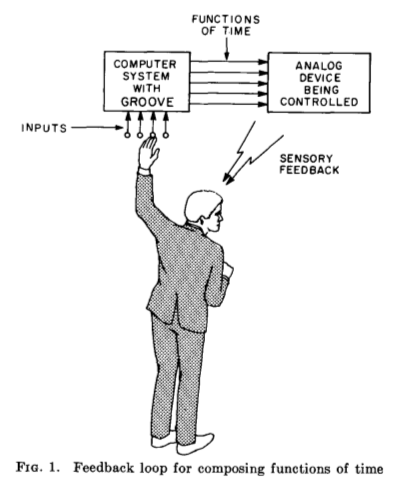
\includegraphics[scale=0.618]{./imagens/GROOVE.png}
\caption{Esquema de concepção do projeto GROOVE. \textbf{Fonte}: \cite{mathews_groove_1970}.}
\label{fig:groove_sistema}
\end{center}
\end{figure} 

O terceiro conceito observa a existência de uma relação entre um humano e uma máquina. Mathews descreve-o como uma \emph{engenharia humana}. Esta engenharia consistiu na observação de um tempo diferencial entre o que o(a) musicista cria e o que edita:

\traduzcitacao{
O conceito final é mais nebuloso. Desde que o GROOVE é um sistema homem-máquina, a engenharia humana do sistema foi a mais importante. Por exemplo, nós descobrimos que o controle do programa de tempo necessita ser bastante diferente para a composição do que para a edição, e o programa foi modificado de acordo. (\ldots) O intérprete de computador não deve tentar definir todo o som em tempo real. Ao invés, o computador deve ter uma partitura e o intérprete deve influenciar a forma como a partitura é tocada. Seus modos de influência podem ser mais variados do que aqueles que um regente convencional, que pode principalmente controloar o tempo, intensidade, e estilo
}
{
The final concept is more nebulous. Since GROOVE is a man-computer system, the human engeneering of the system is most important. For example, we discovered that the control of the program time needs to be quite different for composing than for editing, and the program was modiffied accordingly. (\ldots) The computer performer should not attempt to define the entire sound in real-time. Instead, the computer should have a score and the performer should influence the way in which the score is played. His modes of influence can be much more varied than that a conventional conductor who primarily controls tempo, loudness, and style.
}
{p.~715-716}{mathews_groove_1970}


Como exemplo , selecionamos uma descrição da compositora Laurie \citeonline{spiegel_expanding_1975} (ver \autoref{fig:groove}) para sumarizar as características do GROOVE, durante a produção de \emph{The Expanding Universe} \footnote{Disponível em \url{https://www.youtube.com/watch?v=dYUZmsfm4Ww}.}, entre as salas 2D-506 da Bell Labs (contendo o computador DDP-224) e a sala analógica 2D-562 (laboratório de Mathews). A ``performance'' da obra era realizada, com a programação de funções temporais e a manipulação de parâmetros dessas funções através de dispositivos físicos:

\begin{citacao}
Todas as músicas no GROOVE eram representadas na memória digital como funções abstratas do tempo, séries paralelas de dois pontos, cada ponto sendo um instante no tempo e um valor instantâneo. A taxa de amostragem para essas funções, usada principalmente como controle de voltagem, era cronometrada por um grande e antiquado oscilador analógico que era normalmente fixado em 100 Hertz, cada ciclo do oscilador pulsando à frente do código, o computador lia, em cada uma das funções, naquele ponto do tempo, todos dispositivos de entrada e executava todas amostras. (\ldots) Tínhamos uma pequena caixa com 4 potenciômetros e quatro chaves (alternadores fixados onde você os colocava) e dois botões de disparo.\footnote{Tradução de \emph{All music in GROOVE was represented in digital memory as abstract functions of time, parallel series of point pairs, each point being an instant in time and an instantaneous value. The sampling rate for these functions, which would be used mostly as control voltages, was clocked by a big old-fashioned analog oscillator that was usually set to 100 Hertz, each cycle of the oscillator pulsing one run through the code, the computer reading all of the real time input devices and playing of all of the samples at that time point in each of the time functions. (\ldots)  We had a small box with 4 knobs, 4 set switches (toggles that stay where you put them) and 2 momentary-contact push buttons on it.}}
\end{citacao}

\begin{figure}[!h]
  \begin{center}
  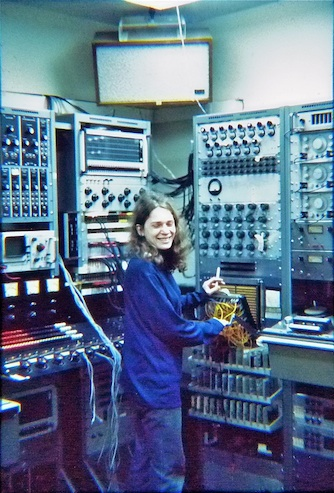
\includegraphics[scale=0.618]{./imagens/spiegel.jpg}
  \caption{\small Laurie Spiegel configurando a saída analógica do GROOVE, durante a produção de \emph{The Expanding Universe}. \textbf{Fonte}: \cite{spiegel_expanding_1975}.}
  \label{fig:groove}
  \end{center}
\end{figure}

Embora não declare ser uma peça minimalista, a descrição de \emph{The Expanding Universe} considera, de maneira asséptica, os fenômenos psicoacústicos como elementos composicionais. Por exemplo, a utilização da continuidade progressiva de sons (ou \emph{drones} transitórios) como elemento criativo permite, segundo a compositora, à sensibilização do ouvido, o que não seria possível na música minimalista instrumental:

\begin{citacao}
 A violência da perturbação sonora, disjunção, descontinuidade e mudanças súbitas desanitizam o ouvinte e nos afastam, de forma que não estamos mais abertos aos sons mais sutis. Mas com continuidade e gentileza, o ouvido se torna re-sensibilizado para mais e mais fenômenos auditoriais sutis dentro do som que estamos imersos. Em vez de sermos arrastados, como nas cascatas de muitas notas executadas em blocos de tempo que mudam repentinamente, tal como tantas vezes consite a música "minimalista", abrimos nossos ouvidos mais e mais para os fenômenos que nos envolvem. Isto também não é música ambiente, um termo que veio a ser usado alguns anos depois. Esta é música para atenção concentrada, uma experiência musical do através, pensando que, lógico, existe também um pano de fundo. \footnote{Tradução de\emph{The violence of sonic disruption, disjunction, discontinuity and sudden change desensitizes the listener and pushes us away so we are no longer open to the subtlest sounds. But with continuity and gentleness, the ear becomes increasingly re-sensitized to more and more subtle auditory phenomena within the sound that immerses us. Instead of being swept along, as with cascades of many running notes in suddenly-changing blocks of time, such as “minimalist” music so often consists of, we open up our ears more and more to the more minute phenomena that envelope us. This is also not “ambient music”, a term that came into use some years later. This is music for concentrated attention, a through-composed musical experience, though of course it also can be background.}}
\end{citacao}

Nesta citação podemos sumarizar um conceito para o \emph{live coding}: Música como um Processo Gradual \cfcite{reich_music_1968}. Porém, o significado de processo pode ser desenvolvido infinitamente. Isso não será realizado. O Processo para Spiegel é diverso daquele considerado no \emph{live coding}, e uma digressão desta pode afastar demais o foco do trabalho principal. Para compreesão deste termo, será necessário explorar outros aspectos correlacionados no decorrer deste trabalho.

Para finalizar esta sessão, a figura \autoref{fig:groove} sugere um conceito rotineiro para o \emph{live coder}. Esta rotina é uma atividade constante de improvisação códigos para aquisição de destreza para uma performance. \citeonline{iazzetta_musica_2009,soares_luteria_2015} lembram que esta atividade, de codificar como se construísse um instrumento musical, se caracteriza por sua conexão com a esfera composicional, nomeado \emph{luteria composicional}.

\section{SuperCollider}\label{sec:supercollider}

O SuperCollider\disponivelem{https://supercollider.github.io/} é um ambiente de programação desenvolvido por James McCartney, lançado em 1996. Segundo \citeonline{mccartney_supercollider_1996}, 

\begin{citacao}
\traducao{SuperCollider começou como dois programas separados que eu escrevi. O primeiro foi um programa chamado \emph{Synth-O-Matic} que era um sintetizador de tempo diferido, escrito de forma semelhante à linguagem C, para Machintosh em 1990 e foi abandonado. O segundo era um objeto \emph{MAX} chamado \emph{Pyrite} que continha um interpretador para a linguagem que se extendeu e foi usado no SuperCollider. Escrever o SuperCollider envolveu integrar uma linguagem interpretada, um coletor delixo $[$administração automática da memória$]$, e uma biblioteca de funções do Pyrite com uma máquina de síntese e funções do Synth-O-Matic. Eu gostaria de agradecer ao Curtis Roads por encorajar-me a reviver o programa do Synth-O-Matic, que levou ao SuperCollider.}{SuperCollider began as two separate programs that I wrote. The first was a program called Synth-O-Matic which was a non-real-time C-like synthesis programming language for the Macintosh written in 1990 and abandoned. The second was a MAX object called Pyrite which contained the interpreter for the language which was extended and used in SuperCollider. Writing SuperCollider involved integrating the language interpreter, garbage collector and function library of Pyrite with the synthesis engine and functions of Synth-O-Matic. I'd like to thank Curtis Roads for encouraging me to revive the Synth-O-Matic program which ultimately led to SuperCollider.}
\end{citacao}

Uma outra perspectiva é oferecida como uma possibilidade lógica e enxuta de outros paradigmas de programação musical.\citeonline[p.~1]{mccartney_supercollider_1996}, descreve alguns problemas com o paradigma de programação musical desenvolvido a partir do Music N \cite{mathews_digital_1963}, como por exemplo, a uma estrutura estática inerente à concepção de objetos conectados por cabos:

\begin{citacao}
\traducao{As abstrações fornecidas pelas linguagens MUSIC N, incluindo o CSound, são abstrações de unidades geradoras, o laço de computação para a amostra de áudio, a representação de conexões entre unidades geradoras, e instanciamento e desalocação de instrumentos. Estas abstrações tornaram a escrita de algoritmos de processamento de sinais mais fácil, porquê eles abstraem um número de detalhes incômodos. Contudo, a família Music N provê poucas estruturas de controle, nenhuma estrutura de dados reais, e nenhuma função de usuário. SAOL melhora o paradigma do Music N provendo tipos de abstrações encontradas na linguagem C, tais como estruturas de controle, funções e algumas estruturas de dados. Max, que é um tipo diferente de linguagem de programação, provê um conjunto interessante de abstrações que permite muitas pessoas usá-lo sem perceberem que estão programando acima de tudo. (\ldots) A linguagem Max també é limitada em sua habilidade de tratar seus objetos como dados, o que torna uma estrutura de objetos estáticos. Evoluções posteriores do Max, como o jMax, e o Pd, fazem várias coisas para expandir as limitações de estrutura de dados do Max, mas ainda assim possuem uma estrutura estática de objeto.
}
{
The abstractions provided by the Music N languages, including Csound (www.csounds.com), are the abstraction of a unit generator, the audio sample computation loop, the representation of the connections between unit generators, and instrument instantiation and de-allocation. These abstractions make writing signal-processing algorithms easier, because they abstract a number of cumbersome details. However, the Music N family provides few control structures, no real data structures, and no user functions. SAOL (www.saol.net) improves the Music N paradigm by providing the kinds of abstractions found in the C language, such as control structures, functions, and some data structures. Max (www.cycling74.com/products/maxmsp.html), which is quite a different kind of programming language, provides an interesting set of abstractions that enable many people to use it
without realizing they are programming at all. (\ldots). The Max language is also limited in its ability to treat its own objects as data, which makes for a static object structure. Later evolutions of Max, such as jMax (www.ircam.fr/produits/logiciels/log-forum/jmax-e.html) and Pd (www.pure-data.org), do various things to expand the data structure limitations of Max but still have a generally static object structure.
}
\end{citacao}

McCartney discute adiante um modelo alternativo de notação musical, adaptado aos padrões de uma linguagem que expresse comportamentos musicais, ao invés da determinação de pontos fixos de parâmetros musicais:

\begin{citacao}
\traducao{Uma lingagem musical de computador deve prover um conjunto de abstralções que expressam idéias composicionais e de processamento de sinais da maneira mais fácil e direta possível. Os tipos de idéias que alguém pode expressar, contudo, podem ser diferentes e levar para diferentes ferramentas. Se alguém interessado em realizar uma partitura que represente uma peça musical como um artefato fixado, então o modelo de partitura/orquestra será suficiente. Motivações que levaram a projetar o SuperCollider estavam na habilidade de perceber processos sonoros que são diferentes, a cada vez que eles são tocados, para escrever peças que de alguma forma descrevem um campo de possibilidades ao invés de uma entidade fixa, e o que facilita a improvisação ao vivo por um compositor/executante.}{A computer music language should provide a set of abstractions that makes expressing compositional and signal processing ideas as easy and direct as possible. The kinds of ideas one wishes to express, however, can be quite different and lead to very different tools. If one is interested in realizing a score that represents a piece of music as a fixed artifact, then a traditional orchestra/score model will suffice. Motivations for the design of SuperCollider were the ability to realize sound processes that were different every time they are played, to write pieces in a way that describes a range of possibilities rather than a fixed entity, and to facilitate live improvisation by a composer/performer.
}
\end{citacao}

Um exemplo de uso pode ilustrar o discurso do McCartney. O exemplo abaixo (p.~\pageref{ex:artificial}) é um código de Fredrik Olofson, outro personagem importante para a improvisação de códigos \cite{ward_live_2004}. Este exemplo é peculiar, uma vez que expõe não somente estruturas dinâmicas e deterministas, mas possibilita criar uma conexão com dois assuntos discutidos anteriormente, algoraves \ver{sec:algorave} e microchips \ver{sec:baiadesaofransisco} .  Um sintetizador recria o timbre do videogame \emph{Atari2600} (laçado no EUA em 1977); mais especificamente é um simulador do \emph{chip} TIA (\emph{Television Interface Adapter}), responsável pela geração de gráficos e imagens no videogame Atari\disponivelem{https://www.atariage.com/2600/archives/schematics_tia/index.html}. O exemplo é relativamente simples. Um sintetizador (\verb|SynthDef|) e um sequenciador (\verb|Pbind|)são definidos. O senquenciador controla parâmetros como as tons, frequências de modulação e panoramização do sintetizador. É interessante notar que padrões fixos (\verb|Pseq| e \verb|Pn|) se misturam com padrões variváveis (\verb|Pbrown|) e segue padrões de movimentos brownianos diferentes que variam entre 28 e 31 $Hz$, alternados com 23 e 26 $Hz$. Enquanto isso a frequência moduladora segue um padrão repetitivo que alterna 10 e 16 $Hz$ com 11 e 16 $Hz$.


\begin{example}{Notação do SuperCollider}
\textbf{Fonte}: \url{http://supercollider.sourceforge.net/audiocode-examples/}

\begin{lstlisting}[style=SuperCollider-IDE]
// Simple synth definition using the Atari2600 UGen:
(
SynthDef(\atari2600, {|out= 0, gate= 1, tone0= 5,
tone1= 8, freq0= 10, freq1= 20, amp= 1, pan= 0|
  var e, z;
  e= EnvGen.kr(Env.asr(0.01, amp, 0.05), gate, doneAction:2);
  z= Atari2600.ar(tone0, tone1, freq0, freq1, 15, 15);
  Out.ar(out, Pan2.ar(z*e, pan));
}).store
)

// And a pattern to play it:
(
Pbind(
  \instrument, \atari2600,
  \dur, Pseq([0.25, 0.25, 0.25, 0.45], inf),
  \amp, 0.8,
  \tone0, Pseq([Pseq([2, 5], 32), Pseq([3, 5], 32)], inf),
  \tone1, 14,
  \freq0, Pseq([Pbrown(28, 31, 1, 32), Pbrown(23, 26, 3, 32)], inf),
  \freq1, Pseq([Pn(10, 16), Pn(11, 16)], inf)
).play
)
\end{lstlisting}
\end{example}\label{ex:artificial}

\subsection{Just In Time Library (JITLib)}\label{sec:jit}

A reflexividade \ver{sec:grossi} é uma característica de diversos ambientes de \emph{live coding}. Segundo \citeonline{aycock_brief_2003}, o primeiros programas JIT foram Genesis (com base no LISP, 1960), LC$^2$ (\emph{Language for Conversational Computing}, 1968) e APL (1970). Este último deu origem ao conceito \emph{lazy evaluation} (avaliação preguiçosa). 

O \emph{SuperCollider} foi o primeiro dos ambientes de programação musical a implementar esta caracterísitca. Com a divulgação da biblioteca JITLib\footnote{Disponível em \url{http://doc.sccode.org/Overviews/JITLib.html}.}, os primeiros Espaços Conceituais do \emph{live coding} se estruturam de maneira bastante formal na comunidade de músicos-programadores. Isto é, durante o ato de codificação podemos codificar a execução de um som antes mesmo de definí-lo (ver \autoref{cod:proxy}).

\begin{example}{Exemplo de avaliação preguiçosa no \emph{Supercollider}.}

Um tipo de variável específica começa com o caractere $~$ para indicar um ambiente propício para a avaliação preguiçosa. Mesmo antes de sua definição, podemos tocar um sintetizador:

  \begin{minted}{c}
    // play some output to the hardware busses,
    // this could be any audio rate key.
    ~out.play;
    ~out = { SinOsc.ar([400, 408] * 0.8, 0, 0.2) };
  \end{minted}

Depois que o código acima é escrito e executado, podemos escrever outros códigos para substituir o sintetizador durante sua execução (\emph{runtime}):
  
  \begin{minted}{c}
    // replacing the node. 
    // the crossfade envelope is created internally.
    ~out = { SinOsc.ar([443, 600 - Rand(0,200)], 0, 0.2) };
    ~out = { Resonz.ar(Saw.ar(40 + [0,0.2], 1), [1200, 1600], 0.1) 
           + SinOsc.ar(60 * [1,1.1],0,0.2) };
    ~out = { Pan2.ar(PinkNoise.ar(0.1), LFClipNoise.kr(2)) };
  \end{minted}
    
  \textbf{Fonte}: \url{http://doc.sccode.org/Tutorials/JITLib/proxyspace_examples.html}
\label{cod:proxy}
\end{example}

Outros \emph{softwares} e ambientes também merecem menção: \emph{ixiLang}\footnote{Disponível em \url{http://www.ixi-audio.net/ixilang/}}\emph{ChucK}\footnote{Disponível em \url{http://chuck.cs.princeton.edu/}.}, \emph{Extempore}\footnote{Disponível em \url{http://benswift.me/extempore-docs/}.}, \emph{Impromptu}\footnote{Disponível em \url{http://impromptu.moso.com.au/}}, \emph{SonicPi}\footnote{Disponível em \url{http://sonic-pi.net/}}

Esta técnica têm sido largamente implementada em navegadores de internet \cite{roberts_web_2013}, ou remotamente \cite{junior_supercopair_2015}. Isto é, entre duas pessoas distantes uma da outra, mas concetadas através da \emph{internet} ou de redes privadas.

Trabalhos neste caminho incluem o Gibber\footnote{Disponível em \url{http://gibber.mat.ucsb.edu/}. \cfcite{roberts_gibber:_2012}} e \emph{Wavepot}\footnote{Disponível em \url{https://www.wavepot.com}.}. Com base neste último, impĺementamos um ambiente chamado \emph{Termpot}\footnote{Disponível em \url{https://jahpd.github.io/termpot}. \cfcite{lunhani_termpot_2015}.}.
\end{apendicesenv}

\phantompart
\printindex
%---------------------------------------------------------------------
\end{document}